% Options for packages loaded elsewhere
\PassOptionsToPackage{unicode}{hyperref}
\PassOptionsToPackage{hyphens}{url}
%
\documentclass[
]{report}
\usepackage{lmodern}
\usepackage{amssymb,amsmath}
\usepackage{ifxetex,ifluatex}
\ifnum 0\ifxetex 1\fi\ifluatex 1\fi=0 % if pdftex
  \usepackage[T1]{fontenc}
  \usepackage[utf8]{inputenc}
  \usepackage{textcomp} % provide euro and other symbols
\else % if luatex or xetex
  \usepackage{unicode-math}
  \defaultfontfeatures{Scale=MatchLowercase}
  \defaultfontfeatures[\rmfamily]{Ligatures=TeX,Scale=1}
\fi
% Use upquote if available, for straight quotes in verbatim environments
\IfFileExists{upquote.sty}{\usepackage{upquote}}{}
\IfFileExists{microtype.sty}{% use microtype if available
  \usepackage[]{microtype}
  \UseMicrotypeSet[protrusion]{basicmath} % disable protrusion for tt fonts
}{}
\makeatletter
\@ifundefined{KOMAClassName}{% if non-KOMA class
  \IfFileExists{parskip.sty}{%
    \usepackage{parskip}
  }{% else
    \setlength{\parindent}{0pt}
    \setlength{\parskip}{6pt plus 2pt minus 1pt}}
}{% if KOMA class
  \KOMAoptions{parskip=half}}
\makeatother
\usepackage{xcolor}
\IfFileExists{xurl.sty}{\usepackage{xurl}}{} % add URL line breaks if available
\IfFileExists{bookmark.sty}{\usepackage{bookmark}}{\usepackage{hyperref}}
\hypersetup{
  pdftitle={  STAT 216 Activity Coursepack},
  pdfauthor={Melinda Yager, Jade Schmidt, Dr.~Stacey Hancock},
  hidelinks,
  pdfcreator={LaTeX via pandoc}}
\urlstyle{same} % disable monospaced font for URLs
\usepackage{color}
\usepackage{fancyvrb}
\newcommand{\VerbBar}{|}
\newcommand{\VERB}{\Verb[commandchars=\\\{\}]}
\DefineVerbatimEnvironment{Highlighting}{Verbatim}{commandchars=\\\{\}}
% Add ',fontsize=\small' for more characters per line
\usepackage{framed}
\definecolor{shadecolor}{RGB}{248,248,248}
\newenvironment{Shaded}{\begin{snugshade}}{\end{snugshade}}
\newcommand{\AlertTok}[1]{\textcolor[rgb]{0.94,0.16,0.16}{#1}}
\newcommand{\AnnotationTok}[1]{\textcolor[rgb]{0.56,0.35,0.01}{\textbf{\textit{#1}}}}
\newcommand{\AttributeTok}[1]{\textcolor[rgb]{0.77,0.63,0.00}{#1}}
\newcommand{\BaseNTok}[1]{\textcolor[rgb]{0.00,0.00,0.81}{#1}}
\newcommand{\BuiltInTok}[1]{#1}
\newcommand{\CharTok}[1]{\textcolor[rgb]{0.31,0.60,0.02}{#1}}
\newcommand{\CommentTok}[1]{\textcolor[rgb]{0.56,0.35,0.01}{\textit{#1}}}
\newcommand{\CommentVarTok}[1]{\textcolor[rgb]{0.56,0.35,0.01}{\textbf{\textit{#1}}}}
\newcommand{\ConstantTok}[1]{\textcolor[rgb]{0.00,0.00,0.00}{#1}}
\newcommand{\ControlFlowTok}[1]{\textcolor[rgb]{0.13,0.29,0.53}{\textbf{#1}}}
\newcommand{\DataTypeTok}[1]{\textcolor[rgb]{0.13,0.29,0.53}{#1}}
\newcommand{\DecValTok}[1]{\textcolor[rgb]{0.00,0.00,0.81}{#1}}
\newcommand{\DocumentationTok}[1]{\textcolor[rgb]{0.56,0.35,0.01}{\textbf{\textit{#1}}}}
\newcommand{\ErrorTok}[1]{\textcolor[rgb]{0.64,0.00,0.00}{\textbf{#1}}}
\newcommand{\ExtensionTok}[1]{#1}
\newcommand{\FloatTok}[1]{\textcolor[rgb]{0.00,0.00,0.81}{#1}}
\newcommand{\FunctionTok}[1]{\textcolor[rgb]{0.00,0.00,0.00}{#1}}
\newcommand{\ImportTok}[1]{#1}
\newcommand{\InformationTok}[1]{\textcolor[rgb]{0.56,0.35,0.01}{\textbf{\textit{#1}}}}
\newcommand{\KeywordTok}[1]{\textcolor[rgb]{0.13,0.29,0.53}{\textbf{#1}}}
\newcommand{\NormalTok}[1]{#1}
\newcommand{\OperatorTok}[1]{\textcolor[rgb]{0.81,0.36,0.00}{\textbf{#1}}}
\newcommand{\OtherTok}[1]{\textcolor[rgb]{0.56,0.35,0.01}{#1}}
\newcommand{\PreprocessorTok}[1]{\textcolor[rgb]{0.56,0.35,0.01}{\textit{#1}}}
\newcommand{\RegionMarkerTok}[1]{#1}
\newcommand{\SpecialCharTok}[1]{\textcolor[rgb]{0.00,0.00,0.00}{#1}}
\newcommand{\SpecialStringTok}[1]{\textcolor[rgb]{0.31,0.60,0.02}{#1}}
\newcommand{\StringTok}[1]{\textcolor[rgb]{0.31,0.60,0.02}{#1}}
\newcommand{\VariableTok}[1]{\textcolor[rgb]{0.00,0.00,0.00}{#1}}
\newcommand{\VerbatimStringTok}[1]{\textcolor[rgb]{0.31,0.60,0.02}{#1}}
\newcommand{\WarningTok}[1]{\textcolor[rgb]{0.56,0.35,0.01}{\textbf{\textit{#1}}}}
\usepackage{longtable,booktabs}
% Correct order of tables after \paragraph or \subparagraph
\usepackage{etoolbox}
\makeatletter
\patchcmd\longtable{\par}{\if@noskipsec\mbox{}\fi\par}{}{}
\makeatother
% Allow footnotes in longtable head/foot
\IfFileExists{footnotehyper.sty}{\usepackage{footnotehyper}}{\usepackage{footnote}}
\makesavenoteenv{longtable}
\usepackage{graphicx}
\makeatletter
\def\maxwidth{\ifdim\Gin@nat@width>\linewidth\linewidth\else\Gin@nat@width\fi}
\def\maxheight{\ifdim\Gin@nat@height>\textheight\textheight\else\Gin@nat@height\fi}
\makeatother
% Scale images if necessary, so that they will not overflow the page
% margins by default, and it is still possible to overwrite the defaults
% using explicit options in \includegraphics[width, height, ...]{}
\setkeys{Gin}{width=\maxwidth,height=\maxheight,keepaspectratio}
% Set default figure placement to htbp
\makeatletter
\def\fps@figure{htbp}
\makeatother
\setlength{\emergencystretch}{3em} % prevent overfull lines
\providecommand{\tightlist}{%
  \setlength{\itemsep}{0pt}\setlength{\parskip}{0pt}}
\setcounter{secnumdepth}{5}
\usepackage{booktabs}
\usepackage{geometry}
\usepackage[none]{hyphenat}
\usepackage{titlesec}
\usepackage{longtable}
\usepackage{longtable}
\usepackage{xcolor}
\usepackage{setspace}

\pagestyle{plain}

%%%% Set margins
\setlength{\topmargin}{-1cm}
\addtolength{\evensidemargin}{-1cm}
\addtolength{\oddsidemargin}{-1cm}
\addtolength{\textheight}{3cm}
\addtolength{\textwidth}{2cm}

% Spacing for reading guides
\newcommand{\rgs}{\vspace{12pt}} % Vertical space
\newcommand{\rgi}{\hspace{20pt}}  % Indent

\renewcommand*{\chaptername}{Chapter}

\titleformat{\chapter}[display]
{\bfseries\Large}
{\filleft\MakeUppercase{\chaptertitlename} \Huge\thechapter}
{3ex}
{\titlerule
\vspace{1.5ex}%
\filright}
[\vspace{1.5ex}%
\titlerule]
\titlespacing*{\chapter}{0pt}{-40pt}{20pt}
\ifluatex
  \usepackage{selnolig}  % disable illegal ligatures
\fi
\usepackage[]{natbib}
\bibliographystyle{plainnat}

\title{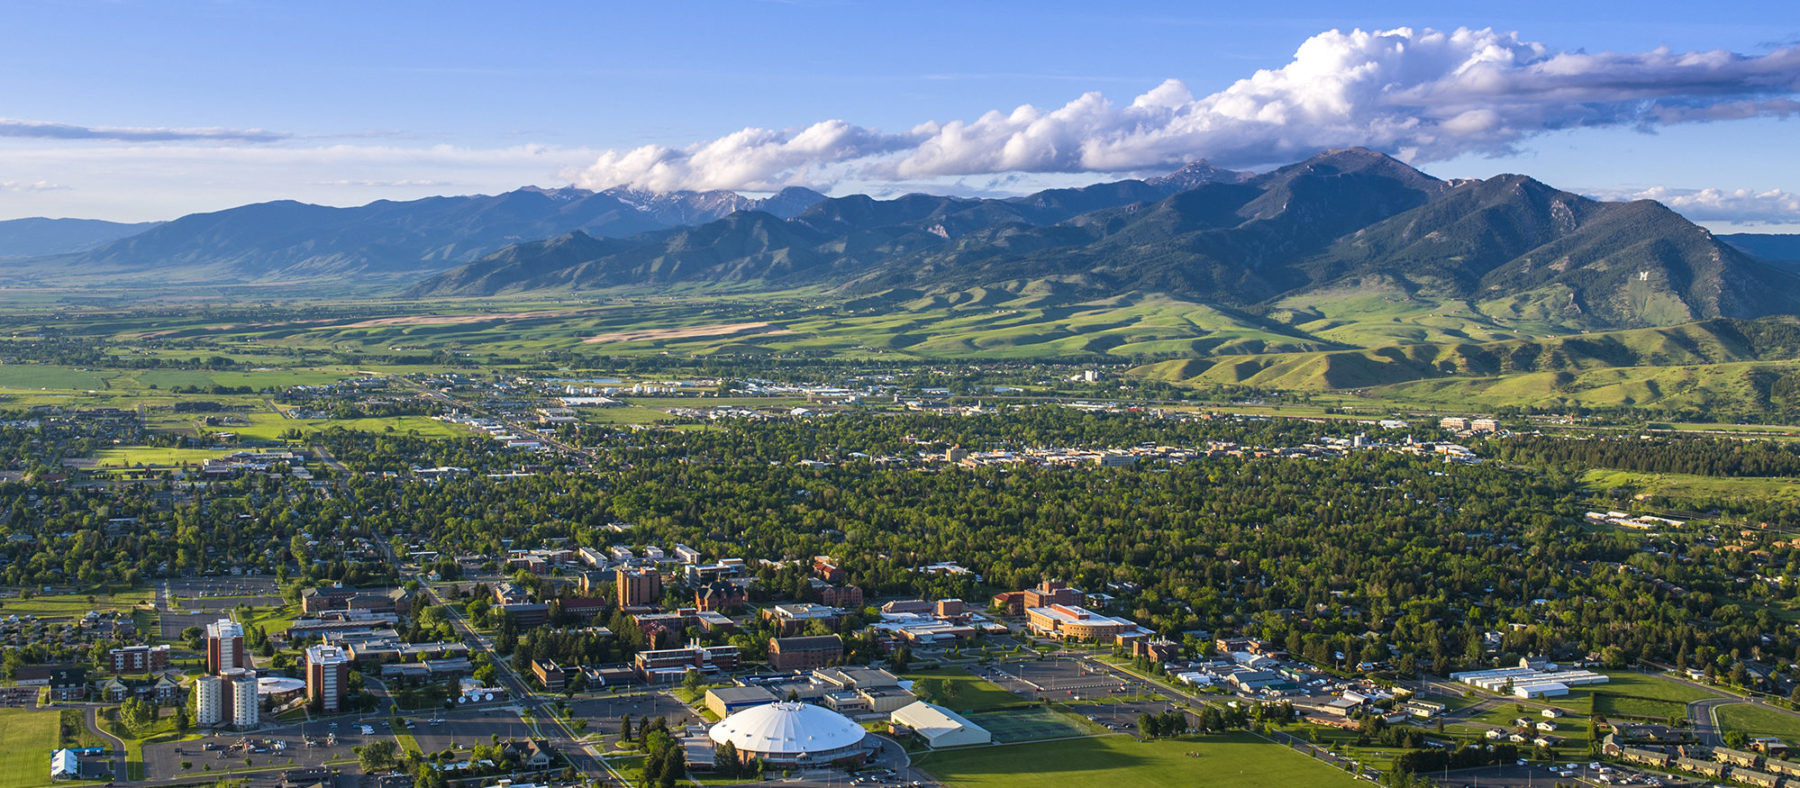
\includegraphics[width=5in,height=\textheight]{images/msu-campus.jpg}
\vspace{1cm}\\
STAT 216 Activity Coursepack}
\usepackage{etoolbox}
\makeatletter
\providecommand{\subtitle}[1]{% add subtitle to \maketitle
  \apptocmd{\@title}{\par {\large #1 \par}}{}{}
}
\makeatother
\subtitle{Spring 2021}
\author{Melinda Yager, Jade Schmidt, Dr.~Stacey Hancock}
\date{}

\begin{document}
\maketitle

\newpage
\thispagestyle{empty}

This resource was developed by Melinda Yager, Jade Schmidt, and Stacey Hancock in 2021 to accompany the online textbook: Carnegie, N., Hancock, S., Meyer, E., Schmidt, J., and Yager, M. (2021). \emph{Montana State Introductory Statistics with R}. Montana State University. \url{https://mtstateintrostats.github.io/IntroStatTextbook/}.

This resource is released under a \href{https://creativecommons.org/licenses/by-nc-sa/4.0/}{Creative Commons BY-NC-SA 4.0} license unless otherwise noted.

\setcounter{tocdepth}{0}
\tableofcontents
\setcounter{page}{1}

\newpage

\hypertarget{preface}{%
\chapter*{Preface}\label{preface}}
\addcontentsline{toc}{chapter}{Preface}

This coursepack accompanies the textbook for STAT 216: Introduction to Statistics at Montana State University. The coursepack includes reading guides to aid in taking notes while you complete the required readings, and in-class activities. Each of the activities in this workbook is designed to target specific learning outcomes of the course, giving you practice with important statistical concepts in a group setting with instructor guidance. Bring this workbook with you to class each week, and take notes in the workbook as you would your own notes. A well-written complete workbook will provide an optimal study guide for exams!

The activities in this coursepack are broken into three sections: pre-class, in-class, and after class. Read through the introduction for each activity and complete the pre-class questions before attending class each week. In class, you will work through the in-class section with your group and instructor. After class, you will complete the out of class part of the activity.

STAT 216 is a 3-credit blended course. Rather than meeting for a total of 150 structured minutes in class per week, students meet with their instructor and cohort of classmates for 50 minutes of class per week. The other 100 minutes typically spent in class are instead spent outside of class watching instructor video lectures, reading the textbook, working through case studies, and participating in online discussion with your classmates. This structure serves two purposes: (1) enhance the safety of our community during the COVID-19 pandemic, and (2) provide additional flexibility for students to create their own schedule and make their own decisions on how they learn best.

In our experience, it takes six to nine hours per week outside of class to achieve a good grade in STAT 216 -- this means six to nine hours outside of the 150 minutes of time set aside for learning course material each week. By ``good'' we mean at least a C because a grade of C- or below does not count toward fulfilling degree requirements. Many of you set your goals higher than just getting a C, and we fully support that. You
need roughly nine hours per week to review past activities, read feedback on previous assignments, complete current assignments, and prepare for the next day's class. A typical week in the life of a STAT 216 student looks like:

\begin{itemize}
\tightlist
\item
  \emph{Prior to weekly class meeting}:

  \begin{itemize}
  \tightlist
  \item
    Read assigned sections of textbook, using the provided reading guides to take notes on the material.
  \item
    Watch assigned videos on that week's content, pausing to take notes and answer video quiz questions.
  \item
    Read through the introduction to the week's in-class activity and complete the pre-class questions.
  \item
    Read through the week's homework assignment and note any questions you may have on the content.
  \end{itemize}
\item
  \emph{In class meeting}:

  \begin{itemize}
  \tightlist
  \item
    Work through in-class activity with your classmates and instructor, taking detailed notes on your answers to each question in the activity.
  \end{itemize}
\item
  \emph{After weekly class meeting}:

  \begin{itemize}
  \tightlist
  \item
    Complete the out-of-class part of the activity, plus any additional parts of the activity you did not complete in class.
  \item
    Review the posted activity solutions and wrap-up videos, and take notes on key points.
  \item
    Finish watching any remaining assigned videos or readings for the week.
  \item
    Read through the week's case study and post case study discussion posts on D2L.
  \item
    Complete the week's homework assignment.
  \end{itemize}
\end{itemize}

\hypertarget{stat-216-syllabus}{%
\chapter*{STAT 216 Syllabus}\label{stat-216-syllabus}}
\addcontentsline{toc}{chapter}{STAT 216 Syllabus}

The course syllabus for STAT 216 can also be found online at \url{https://mtstateintrostats.github.io/Syllabus/}.

TODO: Copy and paste syllabus here once finalized.

\hypertarget{spring-2021-calendar-of-in-class-activities}{%
\chapter*{Spring 2021 Calendar of In-Class Activities}\label{spring-2021-calendar-of-in-class-activities}}
\addcontentsline{toc}{chapter}{Spring 2021 Calendar of In-Class Activities}

\begin{longtable}{|p{.1\textwidth}|l|p{.1\textwidth}|l|p{.40\textwidth}|}
\hline
\textbf{Week}& \textbf{Activity No.}& \textbf{Day}& \textbf{Date}& \textbf{Activity} \\ \hline
\endhead
1& 1& M& 1/11& Martian Alphabet \\*
1& 1& W& 1/13& Martian Alphabet \\*
1& 1& F& 1/15& Martian Alphabet \\ \hline
2& 2& M& 1/18& Study Design \\*
2& 2& W& 1/20& Study Design \\*
2& 2& F& 1/22& Study Design \\ \hline
3& 3& M& 1/25& What's the Probability? \\*
3& 3& W& 1/27& What's the Probability? \\*
3& 3& F& 1/29& What's the Probability? \\ \hline
4& 4& M& 2/1& IMDb Movie Reviews \\*
4& 4& W& 2/3& IMDb Movie Reviews \\*
4& 4& F& 2/5& IMDb Movie Reviews \\ \hline
5& 4& M& 2/8& Movie Profits \\*
5& 5& W& 2/10& Movie Profits \\*	
5& 5& F& 2/12& Movie Profits \\ \hline
6& $-$& M$-$F& 2/15$-$2/19& Exam 1 \\ \hline
7& 6& M& 2/22& Handedness of Male Boxers \\*
7& 6& W& 2/24& Handedness of Male Boxers \\*	
7& 6& F& 2/26& Handedness of Male Boxers \\ \hline
8& 7& M& 3/1& Estimate the Proportion of Left-Handed Male Boxers \\*
8& 7& W& 3/3& Estimate the Proportion of Left-Handed Male Boxers \\*	
8& 7& F& 3/5& Estimate the Proportion of Left-Handed Male Boxers \\ \hline
9& 8& M& 3/8& Winter Sports Helmet Use and Head Injuries \\*
9& 8& W& 3/10& Winter Sports Helmet Use and Head Injuries \\*	
9& 8& F& 3/12& Winter Sports Helmet Use and Head Injuries \\ \hline
10& 9& M& 3/15& Estimate the Difference in Proportion of Head Injuries \\*
10& 9& W& 3/17& Estimate the Difference in Proportion of Head Injuries \\*
10& 9& F& 3/19& Estimate the Difference in Proportion of Head Injuries \\ \hline
11& 10& M& 3/22& COVID-19 and Air Pollution \\*
11& 10& W& 3/24& COVID-19 and Air Pollution \\*	
11& 10& F& 3/26& COVID-19 and Air Pollution \\ \hline
12& 11& M& 3/29& Weather Patterns \\*
12& 11& W& 3/31& Weather Patterns \\*
12& 11& F& 4/2& Weather Patterns \\ \hline
13& 12& M& 4/5& Moneyball \\*
13& 12& W& 4/7& Moneyball \\*
13& 12& F& 4/9& Moneyball \\ \hline
14& $-$& M$-$F& 4/12$-$4/16& Exam 2 \\ \hline
15& $-$& M$-$F& 4/19$-$4/23& Group Projects \\ \hline
\end{longtable}

\hypertarget{reading-guide-1-basics-of-data}{%
\chapter{Reading Guide 1: Basics of Data}\label{reading-guide-1-basics-of-data}}

\hypertarget{sections-1.1-case-study-and-1.2-basics-of-data}{%
\section*{Sections 1.1 (Case Study) and 1.2 (Basics of Data)}\label{sections-1.1-case-study-and-1.2-basics-of-data}}
\addcontentsline{toc}{section}{Sections 1.1 (Case Study) and 1.2 (Basics of Data)}

\hypertarget{vocabulary}{%
\subsection*{Vocabulary}\label{vocabulary}}
\addcontentsline{toc}{subsection}{Vocabulary}

\setstretch{1.25}

Data:
\rgs

Summary statistic:
\rgs

Case/Observational unit:
\rgs

Variable:
\rgs

\rgi Quantitative variable:
\rgs

\rgi Discrete variables:
\rgs

\rgi \rgi Examples of discrete variables using the \texttt{County} data:
\rgs

\rgi Continuous variables:
\rgs

\rgi \rgi Examples of continuous variables using the \texttt{County} data:
\rgs

Example of a number which is NOT a numerical variable:
\rgs

Categorical variable:
\rgs

\rgi Ordinal variable:
\rgs

\rgi \rgi Example of an ordinal variable using the \texttt{County} data:
\rgs

\rgi Nominal variable:
\rgs

\rgi \rgi Examples of nominal variables using the \texttt{County} data:

\rgs

\textbf{Note: Ordinal and nominal variables will be treated the same in this course. We recommend taking more statistics courses in the future to learn better methods of analysis for ordinal variables.}

Data frame:
\rgs

Scatterplot:
\rgs

\rgi Each point represents:

\rgi Positive association:

\rgi Negative association:

Association or Dependent variables:
\rgs

Independent variables:
\rgs

Explanatory variable:
\rgs

Response variable:
\rgs

Observational study:
\rgs

Experiment:
\rgs

Placebo:
\rgs

\hypertarget{notes}{%
\subsection*{Notes}\label{notes}}
\addcontentsline{toc}{subsection}{Notes}

Big Idea: Variability is inevitable! We would not expect to get \emph{exactly} 50 heads in 100 coin flips. The statistical question then is whether any differences found in data are due to random variability, or if something else is going on.

\begin{quote}
The larger the difference, the \textbf{less we believe the difference was due to chance.}
\end{quote}

In a data frame, rows correspond to \_\_\_\_\_\_\_\_\_\_\_\_\_\_\_\_\_\_\_

and columns correspond to \_\_\_\_\_\_\_\_\_\_\_\_\_\_\_\_\_\_.

How many types of variables are discussed? Explain the differences between them and give an example of each.
\rgs
\rgs
\newpage

True or False: A pair of variables be both associated AND independent.\\
True or False: Given a pair of variables, will one always be the explanatory and one the response variable.\\
True or False: If a study does have an explanatory and a response variable, that means changes in the explanatory variable must cause changes in the response variable?\\
True or False: Observational studies can show a naturally occurring association between variables.

\hypertarget{example-section-1.1---case-study-using-stents-to-prevent-strokes}{%
\subsection*{Example (Section 1.1 - Case Study: Using stents to prevent strokes)}\label{example-section-1.1---case-study-using-stents-to-prevent-strokes}}
\addcontentsline{toc}{subsection}{Example (Section 1.1 - Case Study: Using stents to prevent strokes)}

\begin{enumerate}
\def\labelenumi{\arabic{enumi})}
\item
  What is the principle question the researchers hope to answer? (We call this the \textbf{research question}.)
  \rgs
  \rgs
\item
  When creating two groups to compare, do the groups have to be the same size (same number of people in each)?
  \rgs
  \rgs
\item
  What are the cases or observational units in this study?
  \rgs
  \rgs
\item
  Is there a clear explanatory and response variable? If so, name the variable in each role and determine the type of variable (discrete, continuous, nominal, or ordinal).
  \rgs
  \rgs
\item
  What is the purpose of the control group?
  \rgs
  \rgs
\item
  Is this an example of an observational study or an experiment? How do you know?
  \rgs
  \rgs
\item
  Consider Tables 1.1 and 1.2. Which table is more helpful in answering the research question? Justify your answer.
  \rgs
  \rgs
\item
  Describe in words what is shown in Figure 1.1. Specifically, compare the proportion of patients who had a stroke between the treatment and control groups after 30 days as well as after 365 days.
  \rgs
  \rgs
\item
  Given the notion that the larger the difference between the two groups (for a given sample size), the less believable it is that the difference was due to chance, which measurement period (30 days or 365 days) provide stronger evidence that there is an association between stents and strokes, or that the differences are not due to random chance?
  \rgs
  \rgs
\item
  This study reported finding evidence that stents \textbf{increase} the risk of stroke. Does this conclusion apply to all patients and all stents?
  \rgs
  \rgs
\item
  This study reported finding evidence that stents \textbf{increase} the risk of stroke. This conclusion implies a causal link between stents and an increased risk of stroke. Is that conclusion valid? Justify your answer.
\end{enumerate}

\hypertarget{activity-1-martian-alphabet}{%
\chapter{Activity 1: Martian Alphabet}\label{activity-1-martian-alphabet}}

\setstretch{1}

\hypertarget{learning-outcomes}{%
\section{Learning outcomes}\label{learning-outcomes}}

\begin{itemize}
\item
  Describe the statistical investigation process
\item
  Identify observational units, variables, and variable types in a statistical study
\end{itemize}

\hypertarget{terminology-review}{%
\section{Terminology review}\label{terminology-review}}

Statistics is the study of how best to collect, analyze, and draw conclusions from data. Today in class you will be introduced to the following terms:

\begin{itemize}
\item
  Observational units or cases
\item
  Variables: categorical or quantitative
\item
  Proportions
\item
  Graphs: frequency bar plot and relative frequency bar plot
\item
  Distribution
\end{itemize}

For more on these concepts, read Sections 1.2 and 2.1 in the textbook.

\hypertarget{can-you-read-martian}{%
\section{Can you read ``Martian''?}\label{can-you-read-martian}}

How well can humans distinguish one ``Martian'' letter from another? In this week's activity, we'll find out. When shown the two Martian letters, Kiki and Bumba, write down whether you think Bumba is on the left or on the right.
\vspace{2mm}

\begin{enumerate}
\def\labelenumi{\arabic{enumi}.}
\tightlist
\item
  Were you correct or incorrect in identifying Bumba?
\end{enumerate}

\vspace{0.3in}

\hypertarget{steps-of-the-statistical-investigation-process}{%
\subsection*{Steps of the statistical investigation process}\label{steps-of-the-statistical-investigation-process}}
\addcontentsline{toc}{subsection}{Steps of the statistical investigation process}

\textbf{Step 1}: The first step of any statistical investigation is to \emph{ask a research question}. In this study the research question is: can we as a class read Martian? (We will refine this later on!).

\textbf{Step 2}: To answer any research question, we must \emph{design a study and collect data}. For our question, the study consists of each student being presented with two Martian letters and asking which was Bumba. Your responses will become our observed data that we will explore.

\newpage

\textbf{Observational units} or \textbf{cases} are the subjects data are collected on. In a spreadsheet of the data set, each row will represent a single observational unit.

\begin{enumerate}
\def\labelenumi{\arabic{enumi}.}
\setcounter{enumi}{1}
\tightlist
\item
  What are the observational units in this study?
\end{enumerate}

\vspace{0.4in}

\begin{enumerate}
\def\labelenumi{\arabic{enumi}.}
\setcounter{enumi}{2}
\tightlist
\item
  How many students are in class today? This is the \emph{sample size}.
\end{enumerate}

\vspace{0.3in}

A \textbf{variable} is information collected or measured on each observational unit or case. Each column in a data set will represent a different variable. Today we are only measuring one variable on each observational unit.

\begin{enumerate}
\def\labelenumi{\arabic{enumi}.}
\setcounter{enumi}{3}
\tightlist
\item
  Identify the variable we are collecting on each observational unit in this study, i.e., what are we measuring on each student? \emph{Hint}: Your answer to question 1 is the outcome for the variable measured on one observational unit.
\end{enumerate}

\vspace{.8in}

We will look at two types of variables: \textbf{quantitative} and \textbf{categorical} (see Figure \ref{fig:types-of-variables}).

Quantitative variables are numerical measurements that can be discrete (whole, non-negative numbers) or continuous (any value within an interval). The number of pets one owns would be a discrete variable as you can not have a partial pet. GPA would be a continuous variable ranging from 0 to 4.0.

Categorical variables are data that are in groups or categories such as eye color, state of residency, or whether or not a student lives on campus. Categorical variables with a natural ordering are considered ordinal variables while those without a natural ordering are considered nominal variables. All categorical variables will be treated as nominal for analysis in this course.

\begin{figure}

{\centering 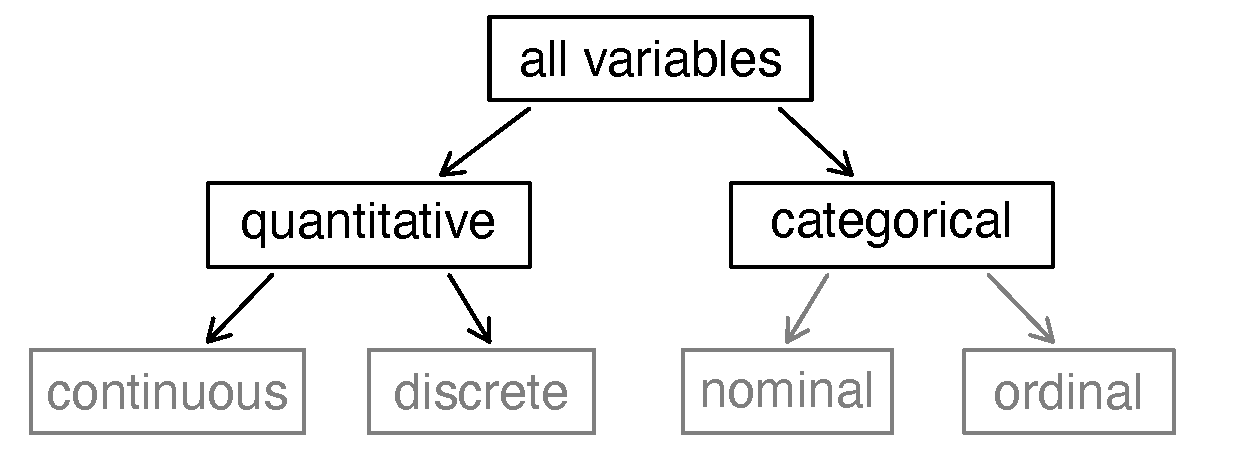
\includegraphics[width=0.6\linewidth]{images/variables} 

}

\caption{Types of variables.}\label{fig:types-of-variables}
\end{figure}

\begin{enumerate}
\def\labelenumi{\arabic{enumi}.}
\setcounter{enumi}{4}
\tightlist
\item
  Is the variable identified in question 4 categorical or quantitative?
\end{enumerate}

\vspace{0.3in}

\newpage

\textbf{Step 3}: Once we have collected data, the next step is to \emph{summarize and visualize the data}.

\begin{enumerate}
\def\labelenumi{\arabic{enumi}.}
\setcounter{enumi}{5}
\tightlist
\item
  How many people in your class were correct in identifying Bumba? Using the class size from question 2, calculate the proportion of students who correctly identified Bumba.
\end{enumerate}

\begin{center}
$\mbox{proportion} = \frac{\mbox{number of students who correctly identified Bumba}}{\mbox{total number of students}}$
\end{center}

\vspace{0.7in}

The proportion in question 6 is called a \textbf{summary statistic}---a single value that summarizes the data set. It is important to note that a variable is different than a summary statistic. A \emph{variable} is measured on a \emph{single observational unit} while a summary statistic is calculated from a group of observational units. For example, the variable ``whether or not a student lives on campus'' can be measured on each individual student. In a class of 50 students we can calculate the proportion of students who live on campus, the summary statistic. Look back and make sure you wrote the variable in question 3 as a variable, NOT a summary statistic.

Looking at the data set and the summary statistic is only one way to display the data. We will also want to create a visualization or picture of the data. A \textbf{frequency bar plot} is used to display categorical data as a count or frequency. Since our variable has two levels or outcomes, correct or incorrect, we will create two bars---one for each level.

\begin{enumerate}
\def\labelenumi{\arabic{enumi}.}
\setcounter{enumi}{6}
\tightlist
\item
  Plot the observed class data using a frequency bar plot. Be sure to add a scale to the y-axis.
\end{enumerate}

\begin{center}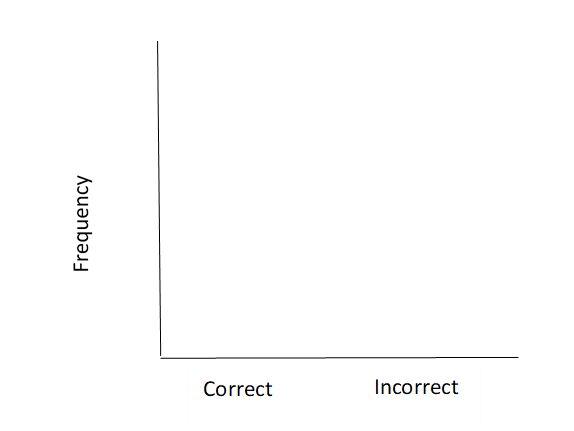
\includegraphics[width=0.4\linewidth]{images/barplot_martian} \end{center}

We can also visualize the data as a proportion in a \textbf{relative frequency bar plot}. Relative frequency is the proportion calculated for each level of the categorical variable.

\begin{enumerate}
\def\labelenumi{\arabic{enumi}.}
\setcounter{enumi}{7}
\tightlist
\item
  Plot the observed class data using a relative frequency bar plot. Be sure to add a scale to the y-axis.
\end{enumerate}

\begin{center}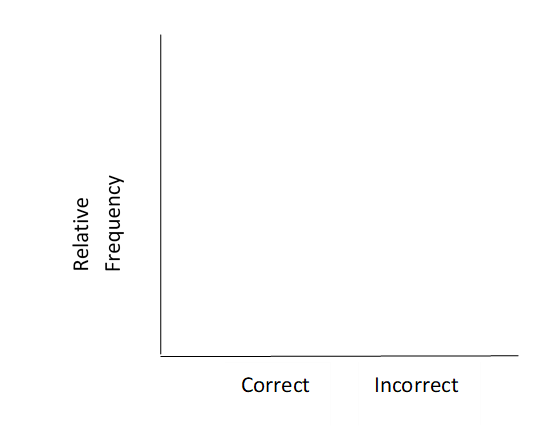
\includegraphics[width=0.4\linewidth]{images/relative_barplot_martian} \end{center}

\newpage

\textbf{Step 4}: The next step is to \emph{use statistical analysis methods to draw inferences from the data}. To answer the research question, we will simulate what \emph{could} have happened in our class given random chance, repeat many times to understand the expected \emph{variability} between different ``randomly guessing'' classes, then compare our class's observed data to the simulation. This gives us an estimate of how often (or the probability of) the class's result would occur if students were all merely guessing, allowing us to determine if the data provides evidence that we as a class can in fact read Martian.

\begin{enumerate}
\def\labelenumi{\arabic{enumi}.}
\setcounter{enumi}{8}
\item
  If humans really don't know Martian and are just guessing which is Bumba, what are the chances of getting it right?
  \vspace{0.3in}

  How could we use a coin to simulate each student ``just guessing'' which Martian letter is Bumba?
  \vspace{.9in}

  How could we use coins to simulate the entire class ``just guessing'' which Martian letter is Bumba?
  \vspace{.9in}

  How many people in your class would you expect to choose Bumba correctly just by chance? Explain your reasoning.
  \vspace{.9in}
\item
  Each student will flip a coin one time to simulate your ``guess''. Let Heads = correct, Tails = incorrect. What was the result of your one simulation?
  \vspace{.3in}

  What was the result from your class's simulation? What proportion of students ``guessed'' correctly in the simulation?
  \vspace{.3in}
\item
  If students really don't know Martian and are just guessing which is Bumba, which seems more unusual: the result from your class's \textbf{simulation} or the observed proportion of students in your class that were correct (this is your summary statistic from question 6)? Explain your reasoning.
\end{enumerate}

\newpage

\begin{enumerate}
\def\labelenumi{\arabic{enumi}.}
\setcounter{enumi}{11}
\tightlist
\item
  While your observed class data is likely far different from the simulated ``just-guessing'' class, comparing our class data to a single simulation does not give enough information. The differences seen could just be due to that set of coin flips! Let's simulate another class. Each student should flip their coin again. What was the result from your class's second simulation? What proportion of students ``guessed'' correctly in the second simulation? Create a plot to compare the two simulated results with the observed class result.
\end{enumerate}

\vspace{1in}

\begin{enumerate}
\def\labelenumi{\arabic{enumi}.}
\setcounter{enumi}{12}
\tightlist
\item
  We still only have a couple of simulations to compare our class data to. It would be much better to be able to see how our class compared to hundreds or thousands of ``just-guessing'' classes. Since we don't want to flip coins all class period, your instructor will use a computer simulation to get 1000 trials. Fill in the following blanks to describe how we would create a simulation of random guessing with 1000 trials (repetitions).
\end{enumerate}

~~~~~~~~~~Probability of correct guesses: \_\_\_\_\_

\vspace{0.05in}

~~~~~~~~~~Sample size: \_\_\_\_\_

\vspace{0.05in}

~~~~~~~~~~Number of repetitions: \_\_\_\_\_

\vspace{0.05in}

\begin{enumerate}
\def\labelenumi{\arabic{enumi}.}
\setcounter{enumi}{13}
\tightlist
\item
  Sketch the distribution displayed by your instructor here. Label each axis appropriately.
\end{enumerate}

\vspace{1.5in}

\begin{enumerate}
\def\labelenumi{\arabic{enumi}.}
\setcounter{enumi}{14}
\tightlist
\item
  Is your class particularly good or bad at Martian? Use the plot in question 14 to explain your answer.
\end{enumerate}

\vspace{.5in}

\begin{enumerate}
\def\labelenumi{\arabic{enumi}.}
\setcounter{enumi}{15}
\tightlist
\item
  Is it \emph{possible} that we could see our class results just by chance if everyone was just guessing? Explain your reasoning.
\end{enumerate}

\vspace{.5in}

\begin{enumerate}
\def\labelenumi{\arabic{enumi}.}
\setcounter{enumi}{16}
\tightlist
\item
  Is it \emph{likely} that we could see our class results just by chance if everyone was just guessing? Explain your reasoning.
\end{enumerate}

\vspace{.5in}

\textbf{Step 5}: The next step in the statistical investigation process is to \emph{communicate the results and answer the research question}.

\begin{enumerate}
\def\labelenumi{\arabic{enumi}.}
\setcounter{enumi}{17}
\tightlist
\item
  Does this activity provide strong evidence that students were not just guessing at random? If so, what do you think is going on here? Can we as a class read Martian?\footnote{Reference for ``Martian alphabet'' is a TED talk given by Vilayanur Ramachandran in 2007. The synesthesia part begins at roughly 17:30 minutes: \texttt{http://www.ted.com/talks/vilayanur\_ramachandran\_on\_your\_mind}.}
\end{enumerate}

\vspace{1in}

\textbf{Step 6}: The final step of any statistical investigation is to \emph{revisit and look ahead}.

\begin{enumerate}
\def\labelenumi{\arabic{enumi}.}
\setcounter{enumi}{18}
\tightlist
\item
  Can you think of any limitations of our study? Can you think of a new topic that might be of interest based on the results of our study?
\end{enumerate}

\vspace{1in}

\hypertarget{take-home-messages}{%
\section{Take home messages}\label{take-home-messages}}

\begin{enumerate}
\def\labelenumi{\arabic{enumi}.}
\item
  In this course we will learn how to evaluate a claim by comparing observed results (classes' ``guesses'' when asked to identify Bumba) to a distribution of many simulated results under an assumption like ``blind guessing.''
\item
  Blind guessing between two outcomes will be correct only about half the time. We can simulate data using a computer program to fit the assumption of blind guessing.
\item
  Unusual observed results will make us doubt the assumptions used to create the simulated distribution. A large number of correct ``guesses'' is evidence that a person was not just blindly guessing.
\end{enumerate}

\newpage

\hypertarget{out-of-class-activity}{%
\section{Out of Class Activity}\label{out-of-class-activity}}

Since this class is taught in a blended format we are only in class one day per week. During class we will complete the in-class activity from the course pack. Outside of class, students will read from the textbook, watch course videos, and complete an out-of-class activity on the other two days of class. To become familiar with the course outline, read through the syllabus, \url{https://mtstateintrostats.github.io/Syllabus/}, the day specific cohort calendar, and watch the Stat 216 Course Tour on D2L before answering the following questions.

\begin{enumerate}
\def\labelenumi{\arabic{enumi}.}
\tightlist
\item
  When are the case study discussion posts due?
\end{enumerate}

\vspace{0.3in}

\begin{enumerate}
\def\labelenumi{\arabic{enumi}.}
\setcounter{enumi}{1}
\tightlist
\item
  For your cohort, what day and time are the weekly assignments due on Gradescope?
\end{enumerate}

\vspace{0.3in}

\begin{enumerate}
\def\labelenumi{\arabic{enumi}.}
\setcounter{enumi}{2}
\tightlist
\item
  For your cohort, when is Exam 1? Exam 2?
\end{enumerate}

\vspace{0.3in}

In Stat 216 we will use the statistical package \texttt{R} to analyze data. Read through the instructions on the syllabus and download \texttt{R} and \texttt{RStudio\ Desktop} to your computer. If you have a Chromebook or have problems installing \texttt{R} and \texttt{RStudio\ Desktop} on your machine, you will need to use \texttt{RStudio\ Cloud} or an MSU virtual machine. Read through the preliminaries chapter in the textbook and watch the video \texttt{RStudio\_GettingStarted} on D2L -\textgreater{} Content -\textgreater{} Primary Resources before completing the following questions.

Open \texttt{RStudio} on your computer. Download the Martian Alphabet \texttt{RScript} file from D2L and open in \texttt{RStudio}. If the file does not open directly, open manually:

\begin{itemize}
\tightlist
\item
  In \texttt{RStudio} click on File in the upper left hand corner, choose Open File, find the downloaded file.
\end{itemize}

If you are using \texttt{RStudioCloud} watch the video \texttt{RStudioCloud\_GettingStarted} on D2L -\textgreater{} Content -\textgreater{} Primary Resources to learn how to open the file in \texttt{RStudioCloud}.

In the Martian Alphabet \texttt{Rscript} file, highlight the first 14 lines of code and click run. This will install the packages needed for this course. We review a few of these packages here.

Throughout the semester we will use the package \texttt{tidyverse} to allow us to use chaining (see Section 1.7 in the textbook for more on this symbol \texttt{\%\textgreater{}\%}.) We will use the package \texttt{ggplot2} to create graphs in \texttt{RStudio}, the package \texttt{mosaic} to use the favstats function to find summary statistics for quantitative variables, and the package \texttt{catstats} starting in Chapter 5 to create simulations. Once you have installed these packages you will only need to use the library function to call each package to use.

The \# sign is not part of the \texttt{R} code.
It is used by these authors to add comments to the \texttt{R} code and explain what each call is telling the program to do.
\texttt{R} will ignore everything after a \# sign when executing the code.

In the Martian Alphabet \texttt{RScript} file for the one proportion test, enter your class size (Q3 from the in-class activity) for sample\_size and the number of students who were correct in identifying Bumba (Q6 from the in-class activity) for as\_extreme\_as in the one\_proportion\_test. Highlight lines 16 - 21 and click run.

\begin{enumerate}
\def\labelenumi{\arabic{enumi}.}
\setcounter{enumi}{3}
\tightlist
\item
  Is the distribution created from this code similar to what you saw in class in Q14?
\end{enumerate}

\vspace{0.3in}

\hypertarget{additional-notes}{%
\section{Additional notes}\label{additional-notes}}

Use this space to summarize your thoughts and take additional notes on this week's activity and material covered, and to write down the names and contact information of your teammates.

\hypertarget{activity-2-study-design}{%
\chapter{Activity 2: Study Design}\label{activity-2-study-design}}

\hypertarget{learning-outcomes}{%
\section{Learning outcomes}\label{learning-outcomes}}

\begin{itemize}
\item
  Explain the purpose of random sampling and its effect on scope of inference
\item
  Explain the purpose of random assignment and its effect on scope of inference
\item
  Identify whether a study design is observational or an experiment
\item
  Identify confounding variables in observational studies and explain why they are confounding
\item
  Identify the types of bias present in a study
\end{itemize}

\hypertarget{terminology-review}{%
\section{Terminology review}\label{terminology-review}}

In this week's activity, we will examine different types of sampling bias and study designs, confounding variables, and how to determine the scope of inference for a study. Some terms covered in this activity are:

\begin{itemize}
\item
  Population
\item
  Sample
\item
  Parameter
\item
  Statistic
\item
  Selection bias
\item
  Response bias
\item
  Non-response bias
\item
  Scope of inference
\item
  Explanatory variable
\item
  Response variable
\item
  Confounding variable
\item
  Experiment
\item
  Observational study
\end{itemize}

To review these concepts, see Sections 1.3 through 1.6 in the textbook.

\newpage

\hypertarget{types-of-sampling-bias-complete-q1-before-class.}{%
\section{Types of sampling bias: Complete Q1 before class.}\label{types-of-sampling-bias-complete-q1-before-class.}}

There are two parts to study design: how the sample was selected and how the study was conducted. First, we will look at sampling and types of bias (selection, non-response, or response).

In these next questions, identify the target population, the sample selected, the variable, and the type of bias present.

\begin{enumerate}
\def\labelenumi{\arabic{enumi}.}
\item
  To determine if the proportion of out-of-state undergraduate students at Montana State University has increased in the last 10 years, a statistics instructor sent an email survey to 500 randomly selected current undergraduate students. One of the questions on the survey asked whether they had in-state or out-of-state residency. She only received 378 responses.
  \vspace{0.25in}

  Target population:
  \vspace{0.3in}

  Sample:
  \vspace{0.3in}

  Variable:
  \vspace{0.3in}

  Type(s) of bias:
  \vspace{0.3in}
\item
  Pew Research surveys US adults about many different topics. Recently, a survey was conducted to assess current presidential approval. A random sample of 6395 US adults was taken. One of the questions asked in the survey was, ``Do you agree or disagree with President Trump on many or nearly all of the top issues facing the country today?'' Of those surveyed, 42\% said they did agree.
  \vspace{0.25in}

  Target population:
  \vspace{0.3in}

  Sample:
  \vspace{0.3in}

  Variable:
  \vspace{0.3in}

  Type(s) of bias:
  \vspace{0.3in}
\end{enumerate}

\newpage

\begin{enumerate}
\def\labelenumi{\arabic{enumi}.}
\setcounter{enumi}{2}
\item
  A television station is interested in predicting whether or not a local referendum to legalize marijuana for adult use will pass. It asks its viewers to phone in and indicate whether they are in favor or opposed to the referendum. Of the 2241 viewers who phoned in, forty-five percent were opposed to legalizing marijuana.
  \vspace{0.1in}

  Target population:
  \vspace{0.3in}

  Sample:
  \vspace{0.3in}

  Variable:
  \vspace{0.3in}

  Type(s) of bias:
  \vspace{0.3in}
\item
  To gauge the interest in a new swimming pool, a local organization stood outside of the Bogart Pool in Bozeman, MT during open hours. One of the questions they asked was, ``Since the Bogart Pool is in such bad repair, don't you agree that the city should fund a new pool?''
  \vspace{0.1in}

  Target population:
  \vspace{0.3in}

  Sample:
  \vspace{0.3in}

  Variable:
  \vspace{0.3in}

  Type(s) of bias:
  \vspace{0.3in}
\end{enumerate}

\newpage

\hypertarget{study-design}{%
\section{Study design}\label{study-design}}

The two main study designs we will cover are \textbf{observational studies} and \textbf{experiments}. Both the sampling method and the study design will help to determine the \textbf{scope of inference} for a study. Remember that only in a randomized experiment can we conclude a \textbf{causal} (cause and effect) relationship between the explanatory and response variable.

\begin{center}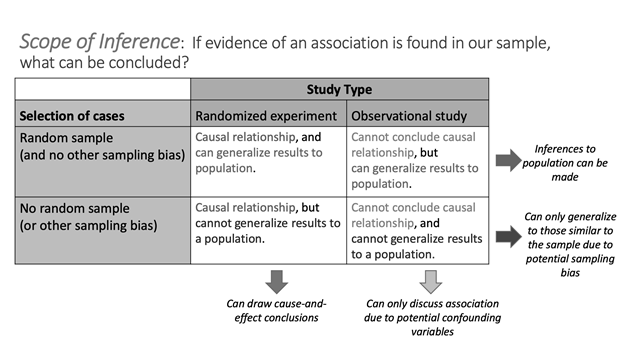
\includegraphics[width=0.75\linewidth]{images/ScopeOfInferenceGreyscale} \end{center}

For the next exercises, identify the explanatory variable, the response variable, the study design (observational study or experiment), and the scope of inference (using the above chart).

\begin{enumerate}
\def\labelenumi{\arabic{enumi}.}
\setcounter{enumi}{4}
\item
  The pharmaceutical company Moderna Therapeutics is working in conjunction with the National Institutes of Health towards a vaccine for COVID-19 and has recently begun Phase 3 clinical trials. US clinical research sites will enroll 30,000 volunteers without COVID-19 to participate. Participants will be randomly assigned to receive either the candidate vaccine or a saline placebo. They will then be followed to assess whether or not they develop COVID-19. The trial is double-blind, so neither the investigators nor the participants will know who is assigned to which group.
  \vspace{0.1in}

  Explanatory variable:
  \vspace{0.25in}

  Response variable:
  \vspace{0.25in}

  Study design:
  \vspace{0.25in}

  What is the scope of inference for this study?
  \vspace{0.5in}
\end{enumerate}

\newpage

\begin{enumerate}
\def\labelenumi{\arabic{enumi}.}
\setcounter{enumi}{5}
\item
  In another study, a local health department randomly selected 1000 US adults without COVID-19 to participate in a health survey. Each participant was assessed at the beginning of the study and then followed for one year. They were interested to see which participants elected to receive a vaccination for COVID-19 and whether any participants developed COVID-19.
  \vspace{0.1in}

  Explanatory variable:
  \vspace{0.25in}

  Response variable:
  \vspace{0.25in}

  Study design:
  \vspace{0.25in}

  What is the scope of inference for this study?
  \vspace{0.5in}
\end{enumerate}

A \textbf{confounding variable} is a variable that is \emph{both}

\begin{enumerate}
\def\labelenumi{\arabic{enumi}.}
\tightlist
\item
  associated with the explanatory variable, \emph{and}
\item
  associated with the response variable.
\end{enumerate}

When both these conditions are met, if we observe an association between the explanatory variable and the response variable in the data, we cannot be sure if this association is due to the explanatory variable or the confounding variable---the explanatory and confounding variables are ``confounded.''

\begin{center}\includegraphics[width=0.7\linewidth]{02-study-design_files/figure-latex/unnamed-chunk-2-1} \end{center}

\begin{enumerate}
\def\labelenumi{\arabic{enumi}.}
\setcounter{enumi}{6}
\tightlist
\item
  For each of the studies in questions 5 and 6, determine whether confounding variables could be an issue. If so, identify a potential confounding variable and explain how it meets the definition of a confounding variable.
  \vspace{1.5in}
\end{enumerate}

\hypertarget{out-of-class-activity}{%
\section{Out of Class Activity}\label{out-of-class-activity}}

In the in-class activity we looked at sampling methods and study design. Here are a few more questions to review that material.

\begin{enumerate}
\def\labelenumi{\arabic{enumi}.}
\item
  The Bozeman school district is interested in surveying parents of students about their opinions on returning to in-person classes following the COVID-19 pandemic. They divided the school district into 10 divisions based on location and randomly surveyed 20 households within each division. Explain why selection bias would be present in this study design.
  \vspace{1in}
\item
  A study published in 2007 by Christopher Johnson, professor of music education and music therapy at the University of Kansas, revealed that students in elementary schools with superior music education programs scored around 20 percent higher in math scores on standardized tests, compared to schools with low-quality music programs. Explain how school budget could be a potential confounding variable. Be sure to address how the confounding variable is related to both the explanatory and response variable.
\end{enumerate}

\vspace{1in}

\begin{enumerate}
\def\labelenumi{\arabic{enumi}.}
\setcounter{enumi}{2}
\tightlist
\item
  What is the purpose of random selection of a sample from the population?
\end{enumerate}

\vspace{1in}

\begin{enumerate}
\def\labelenumi{\arabic{enumi}.}
\setcounter{enumi}{3}
\tightlist
\item
  What is the purpose of random assignment of the cases in a study to the explanatory variable groups?
\end{enumerate}

\vspace{1in}

\newpage

\hypertarget{additional-notes}{%
\section{Additional notes}\label{additional-notes}}

Use this space to summarize your thoughts and take additional notes on this week's activity and material covered.

\hypertarget{activity-3-whats-the-probability}{%
\chapter{Activity 3: What's the probability?}\label{activity-3-whats-the-probability}}

\hypertarget{learning-outcomes}{%
\section{Learning outcomes}\label{learning-outcomes}}

\begin{itemize}
\item
  Recognize and simulate probabilities as long-run frequencies
\item
  Construct two-way tables to evaluate conditional probabilities
\item
  Identify and create appropriate summary statistics and plots
  given a data set or research question
\item
  Plots for a single categorical variable: bar plot
\item
  Plots for association between two categorical variables:
  segmented bar plot, mosaic plot
\end{itemize}

\hypertarget{terminology-review}{%
\section{Terminology review}\label{terminology-review}}

In this week's in-class activity, we will cover two-way tables and probability. In the out of class activity, we will review summary measures and plots for categorical variables. Some terms covered in this activity are:

\begin{itemize}
\item
  Proportions
\item
  Bar plots
\item
  Segmented bar plots
\item
  Probability
\item
  Conditional probability
\item
  Two-way tables
\end{itemize}

To review these concepts, see Sections 2.1 and 2.2 in the textbook.

\newpage

\hypertarget{current-population-survey-1985}{%
\section{``Current'' Population Survey: 1985}\label{current-population-survey-1985}}

The Current Population Survey (CPS) in 1985 is a survey sponsored by the Census Bureau and the Bureau of Labor Statistics to track labor force statistics for the United States population. The following table describes the variables in the data set:

\begin{longtable}[]{@{}ll@{}}
\toprule
\begin{minipage}[b]{0.11\columnwidth}\raggedright
\textbf{Variable}\strut
\end{minipage} & \begin{minipage}[b]{0.83\columnwidth}\raggedright
\textbf{Description}\strut
\end{minipage}\tabularnewline
\midrule
\endhead
\begin{minipage}[t]{0.11\columnwidth}\raggedright
\texttt{educ}\strut
\end{minipage} & \begin{minipage}[t]{0.83\columnwidth}\raggedright
Number of years of education\strut
\end{minipage}\tabularnewline
\begin{minipage}[t]{0.11\columnwidth}\raggedright
\texttt{south}\strut
\end{minipage} & \begin{minipage}[t]{0.83\columnwidth}\raggedright
Whether lives in southern region of the US: \texttt{S} = lives in south, \texttt{NS} = does not live in south\strut
\end{minipage}\tabularnewline
\begin{minipage}[t]{0.11\columnwidth}\raggedright
\texttt{sex}\strut
\end{minipage} & \begin{minipage}[t]{0.83\columnwidth}\raggedright
Sex: \texttt{M} = male, \texttt{F} = female\strut
\end{minipage}\tabularnewline
\begin{minipage}[t]{0.11\columnwidth}\raggedright
\texttt{exper}\strut
\end{minipage} & \begin{minipage}[t]{0.83\columnwidth}\raggedright
Number of years of work experience (inferred from age and education)\strut
\end{minipage}\tabularnewline
\begin{minipage}[t]{0.11\columnwidth}\raggedright
\texttt{union}\strut
\end{minipage} & \begin{minipage}[t]{0.83\columnwidth}\raggedright
Whether union member: \texttt{Union} or \texttt{Not}\strut
\end{minipage}\tabularnewline
\begin{minipage}[t]{0.11\columnwidth}\raggedright
\texttt{wage}\strut
\end{minipage} & \begin{minipage}[t]{0.83\columnwidth}\raggedright
Wage (dollars per hour)\strut
\end{minipage}\tabularnewline
\begin{minipage}[t]{0.11\columnwidth}\raggedright
\texttt{age}\strut
\end{minipage} & \begin{minipage}[t]{0.83\columnwidth}\raggedright
Age (years)\strut
\end{minipage}\tabularnewline
\begin{minipage}[t]{0.11\columnwidth}\raggedright
\texttt{race}\strut
\end{minipage} & \begin{minipage}[t]{0.83\columnwidth}\raggedright
Race: \texttt{W} = white, \texttt{NW} = not white \textbar{}\strut
\end{minipage}\tabularnewline
\begin{minipage}[t]{0.11\columnwidth}\raggedright
\texttt{sector}\strut
\end{minipage} & \begin{minipage}[t]{0.83\columnwidth}\raggedright
Sector of the economy: \texttt{clerical}, \texttt{const} (construction), \texttt{management}, \texttt{manufacturing}, \texttt{professional}, \texttt{sales}, \texttt{service}, \texttt{other}\strut
\end{minipage}\tabularnewline
\begin{minipage}[t]{0.11\columnwidth}\raggedright
\texttt{married}\strut
\end{minipage} & \begin{minipage}[t]{0.83\columnwidth}\raggedright
Marital status: \texttt{Married} or \texttt{Single}\strut
\end{minipage}\tabularnewline
\bottomrule
\end{longtable}

\hypertarget{vocabulary-review.-complete-q1---3-before-class.}{%
\subsection*{Vocabulary review. Complete Q1 - 3 before class.}\label{vocabulary-review.-complete-q1---3-before-class.}}
\addcontentsline{toc}{subsection}{Vocabulary review. Complete Q1 - 3 before class.}

\begin{enumerate}
\def\labelenumi{\arabic{enumi}.}
\tightlist
\item
  What are the observational units?
\end{enumerate}

\vspace{0.5in}

\begin{enumerate}
\def\labelenumi{\arabic{enumi}.}
\setcounter{enumi}{1}
\tightlist
\item
  Which variables are categorical?
\end{enumerate}

\vspace{1in}

\begin{enumerate}
\def\labelenumi{\arabic{enumi}.}
\setcounter{enumi}{2}
\tightlist
\item
  What types of plot can be used to display a single categorical variable? Two categorical variables?
\end{enumerate}

\newpage

\hypertarget{probability}{%
\section{Probability}\label{probability}}

\begin{enumerate}
\def\labelenumi{\arabic{enumi}.}
\setcounter{enumi}{3}
\item
  Since the early 1980s, the rapid antigen detection test (RADT) of group A \emph{streptococci} has been used to detect strep throat. A recent study of the accuracy of this test shows that the sensitivity, the probability of a positive RADT given the person has strep throat, is 86\% in children, while the specificity, the probability of a negative RADT given the person does not have strep throat, is 92\% in children. The prevalence, the probability of having group A strep, is 37\% in children.
  \vspace{1mm}

  Let A = the event the child has strep throat, and B = the event the child has a positive RADT.
  \vspace{0.1in}
\end{enumerate}

\begin{enumerate}
\def\labelenumi{\alph{enumi}.}
\tightlist
\item
  Identify what each numerical value given in the problem represents in probability notation.
  \vspace{.1in}
\end{enumerate}

~~~~~~~~~~~~~~~~0.86 = \vspace{.1in}\\
\hspace*{0.333em}\hspace*{0.333em}\hspace*{0.333em}\hspace*{0.333em}\hspace*{0.333em}\hspace*{0.333em}\hspace*{0.333em}\hspace*{0.333em}\hspace*{0.333em}\hspace*{0.333em}\hspace*{0.333em}\hspace*{0.333em}\hspace*{0.333em}\hspace*{0.333em}\hspace*{0.333em}\hspace*{0.333em}0.92 =

\vspace{.1in}

~~~~~~~~~~~~~~~~0.37 =

\vspace{.1in}

\begin{enumerate}
\def\labelenumi{\alph{enumi}.}
\setcounter{enumi}{1}
\tightlist
\item
  Create a hypothetical two-way table to represent the situation. Recall that in a two-way table, the explanatory variable should be your column headers (similar to the \(x\)-axis in a segmented bar graph!) while the response variable becomes the row headers.
\end{enumerate}

\begin{longtable}[]{@{}llll@{}}
\toprule
\hspace{1in} & \hspace{1in} & \hspace{1in} & Total\tabularnewline
\midrule
\endhead
\hspace{1in} & & &\tabularnewline
\hspace{1in} & & &\tabularnewline
\hspace{1in} & & &\tabularnewline
Total & & & 100,000\tabularnewline
\bottomrule
\end{longtable}

\begin{enumerate}
\def\labelenumi{\alph{enumi}.}
\setcounter{enumi}{2}
\item
  Find \(P(\mbox{A and B})\). What does this probability represent in the context of the problem?
  \vspace{.8in}
\item
  Find the probability that a child with a positive RADT actually has strep throat. What is the notation used for this probability?
\end{enumerate}

\vspace{.8in}

\begin{enumerate}
\def\labelenumi{\alph{enumi}.}
\setcounter{enumi}{4}
\tightlist
\item
  What is the probability that a child does not have strep given that they have a positive test? What is the notation used for this probability?
\end{enumerate}

\newpage

\begin{enumerate}
\def\labelenumi{\arabic{enumi}.}
\setcounter{enumi}{4}
\item
  In a computer store, 30\% of the computers in stock are laptops and 70\% are desktops. Five percent of the laptops are on sale, while 10\% of the desktops are on sale.
  \vspace{1mm}

  Let L = the event the computer is a laptop, and S = the event the computer is on sale.
  \vspace{0.1in}

  \begin{enumerate}
  \def\labelenumii{\alph{enumii}.}
  \tightlist
  \item
    Identify what each numerical value given in the problem represents in probability notation.
    \vspace{.1in}
  \end{enumerate}
\end{enumerate}

~~~~~~~~~~~~~~~~0.30 = \vspace{.1in}\\
\hspace*{0.333em}\hspace*{0.333em}\hspace*{0.333em}\hspace*{0.333em}\hspace*{0.333em}\hspace*{0.333em}\hspace*{0.333em}\hspace*{0.333em}\hspace*{0.333em}\hspace*{0.333em}\hspace*{0.333em}\hspace*{0.333em}\hspace*{0.333em}\hspace*{0.333em}\hspace*{0.333em}\hspace*{0.333em}0.70 =

\vspace{.1in}

~~~~~~~~~~~~~~~~0.05 =

\vspace{.1in}

~~~~~~~~~~~~~~~~0.10 =

\vspace{.1in}

\begin{enumerate}
\def\labelenumi{\alph{enumi}.}
\setcounter{enumi}{1}
\tightlist
\item
  Create a hypothetical two-way table to represent the situation.
\end{enumerate}

\begin{longtable}[]{@{}llll@{}}
\toprule
\hspace{1in} & \hspace{1in} & \hspace{1in} & Total\tabularnewline
\midrule
\endhead
\hspace{1in} & & &\tabularnewline
\hspace{1in} & & &\tabularnewline
\hspace{1in} & & &\tabularnewline
Total & & & 100,000\tabularnewline
\bottomrule
\end{longtable}

\begin{enumerate}
\def\labelenumi{\alph{enumi}.}
\setcounter{enumi}{2}
\item
  Calculate the probability that a randomly selected computer will be a desktop, given that the computer is on sale. What is the notation used for this probability?
  \vspace{.8in}
\item
  Find \(P(S^C | L^C)\). What does this probability represent in context of the problem?
  \vspace{1in}
\item
  What is the probability a randomly selected computer is both a laptop and on sale? Give the appropriate probability notation.
  \newpage
\end{enumerate}

\hypertarget{out-of-class-activity}{%
\section{Out of class activity}\label{out-of-class-activity}}

For this part of the activity we will focus on using \texttt{RStudio} and the provided \texttt{RScript} file to create graphs and calculate proportions from each group.

\hypertarget{nightlight-use-and-myopia}{%
\subsection{Nightlight use and myopia}\label{nightlight-use-and-myopia}}

In a study reported in Nature (1999, Vol. 399, pp.~113-114), a survey of 479 children found that those who had slept with a nightlight or in a fully lit room before the age of 2 had a higher incidence of nearsightedness (myopia) later in childhood.

In this study, there are two variables studied: \texttt{Light}: level of light in room at night (no light, night light, full light) and \texttt{Sight}: level of myopia developed later in childhood (high myopia, myopia, no myopia).

An important part of understanding data is to create visual pictures of what the data represent. In this activity, we will create graphical representations of categorical data.

\hypertarget{r-code}{%
\subsection*{\texorpdfstring{\texttt{R} code}{R code}}\label{r-code}}
\addcontentsline{toc}{subsection}{\texttt{R} code}

Throughout these activities, we will often include the \texttt{R} code
you would use in order to produce output or plots. These
``code chunks'' appear in gray. In the code chunk below, we
demonstrate how to read the data set into \texttt{R} using the \texttt{read.csv()} function.

Open the provided \texttt{RScript} file for activity 3 in \texttt{RStudio} or \texttt{RStudioCloud} to answer the following questions. Highlight and run lines 1 - 5. These lines of code read in the data set and name the data set myopia. The library function tells \texttt{R} which packages will be needed.

\begin{Shaded}
\begin{Highlighting}[]
\CommentTok{\#This will read in the data set}
\NormalTok{myopia \textless{}{-}}\StringTok{ }\KeywordTok{read.csv}\NormalTok{(}\StringTok{"https://math.montana.edu/courses/s216/data/ChildrenLightSight.csv"}\NormalTok{) }
\end{Highlighting}
\end{Shaded}

\hypertarget{displaying-a-single-categorical-variable}{%
\subsection*{Displaying a single categorical variable}\label{displaying-a-single-categorical-variable}}
\addcontentsline{toc}{subsection}{Displaying a single categorical variable}

If we wanted to know how many children in our data set were in each level of myopia, we would create a frequency bar plot of the variable \texttt{Sight}. Enter the variable name, \texttt{Sight}, for xx into the ggplot code in line 10 in the \texttt{RScript} file to create a bar plot. Highlight and run lines 9 - 15. Notice this is a \textbf{frequency} bar plot plotting counts (the number of children in each level of sight).

\begin{Shaded}
\begin{Highlighting}[]
\NormalTok{myopia }\OperatorTok{\%\textgreater{}\%}\StringTok{ }\CommentTok{\#Data set piped into...}
\KeywordTok{ggplot}\NormalTok{(}\KeywordTok{aes}\NormalTok{(}\DataTypeTok{y =}\NormalTok{ xx)) }\OperatorTok{+}\StringTok{   }\CommentTok{\#This specifies the variable}
\StringTok{  }\KeywordTok{geom\_bar}\NormalTok{(}\DataTypeTok{stat =} \StringTok{"count"}\NormalTok{) }\OperatorTok{+}\StringTok{  }\CommentTok{\#Tell it to make a bar plot}
\StringTok{  }\KeywordTok{labs}\NormalTok{(}\DataTypeTok{title =} \StringTok{"Frequency Bar Plot of Level of Myopia"}\NormalTok{,  }\CommentTok{\#Give your plot a title}
       \DataTypeTok{x =} \StringTok{"Frequency"}\NormalTok{,   }\CommentTok{\#Label the x axis}
       \DataTypeTok{y =} \StringTok{"Level of Myopia"}\NormalTok{)  }\OperatorTok{+}\StringTok{ }\CommentTok{\#Label the y axis}
\StringTok{  }\KeywordTok{coord\_flip}\NormalTok{()  }\CommentTok{\#Turn the bars so they are vertical}
\end{Highlighting}
\end{Shaded}

\newpage

\begin{enumerate}
\def\labelenumi{\arabic{enumi}.}
\tightlist
\item
  Sketch the bar plot created here. Be sure to label the axes.
\end{enumerate}

\vspace{1.5in}

\begin{enumerate}
\def\labelenumi{\arabic{enumi}.}
\setcounter{enumi}{1}
\tightlist
\item
  Using the bar chart created, estimate how many children have some level of myopia.
\end{enumerate}

\vspace{0.3in}

We could also choose to display the data as a proportion in a relative frequency bar plot. To find the relative frequency, divide the count in each level of myopia by the sample size. These are sample proportions. Notice that in this code we told \texttt{R} to create a bar plot with proportions.

\begin{Shaded}
\begin{Highlighting}[]
\NormalTok{myopia }\OperatorTok{\%\textgreater{}\%}\StringTok{ }\CommentTok{\#Data set piped into...}
\KeywordTok{ggplot}\NormalTok{(}\KeywordTok{aes}\NormalTok{(}\DataTypeTok{x =}\NormalTok{ Sight)) }\OperatorTok{+}\StringTok{   }\CommentTok{\#This specifies the variable}
\StringTok{  }\KeywordTok{geom\_bar}\NormalTok{(}\KeywordTok{aes}\NormalTok{(}\DataTypeTok{y =}\NormalTok{ ..prop.., }\DataTypeTok{group =} \DecValTok{1}\NormalTok{)) }\OperatorTok{+}\StringTok{  }\CommentTok{\#Tell it to make a bar plot with proportions}
\StringTok{  }\KeywordTok{labs}\NormalTok{(}\DataTypeTok{title =} \StringTok{"Relative Frequency Bar Plot of Level of Myopia"}\NormalTok{,  }\CommentTok{\#Give your plot a title}
       \DataTypeTok{x =} \StringTok{"Level of Myopia"}\NormalTok{,   }\CommentTok{\#Label the x axis}
       \DataTypeTok{y =} \StringTok{"Relative Frequency"}\NormalTok{)  }\CommentTok{\#Label the y axis}
\end{Highlighting}
\end{Shaded}

\begin{center}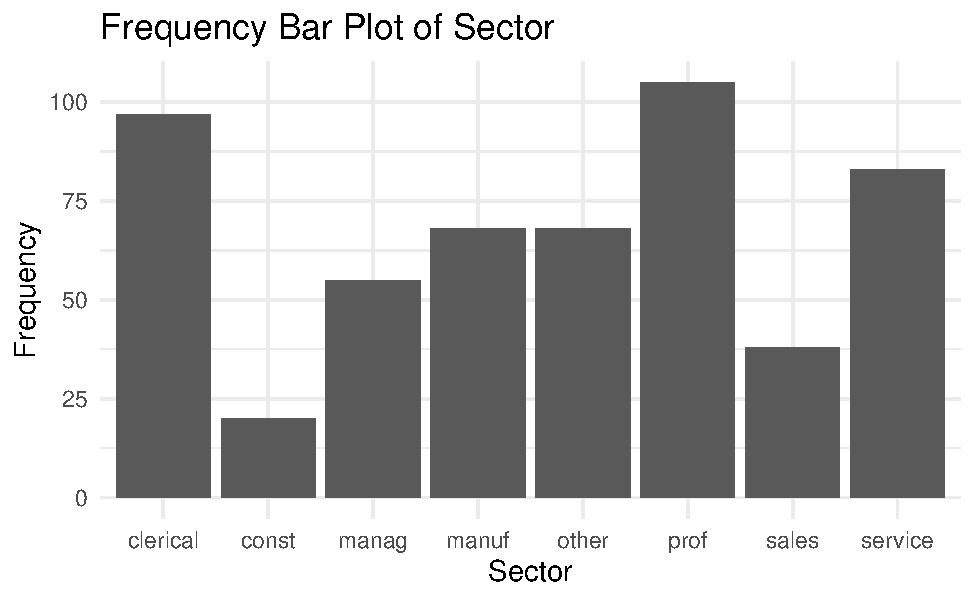
\includegraphics[width=0.5\linewidth]{03-EDA-categorical_files/figure-latex/unnamed-chunk-3-1} \end{center}

\begin{enumerate}
\def\labelenumi{\arabic{enumi}.}
\setcounter{enumi}{2}
\tightlist
\item
  Which features in the relative frequency bar plot are the same as the frequency bar plot? Which are different?
\end{enumerate}

\vspace{1in}

\newpage

\hypertarget{displaying-two-categorical-variables}{%
\subsection*{Displaying two categorical variables}\label{displaying-two-categorical-variables}}
\addcontentsline{toc}{subsection}{Displaying two categorical variables}

To examine the differences in level of myopia for the level of light, we would create a segmented bar plot of \texttt{Light} segmented by \texttt{Sight}. To create the segmented bar plot enter the variable name, \texttt{Light} (explanatory variable) for xx and the variable name, \texttt{Sight} (response variable) for yy in the \texttt{RScript} file in line 28. Highlight and run lines 27 - 33.

\begin{Shaded}
\begin{Highlighting}[]
\NormalTok{myopia }\OperatorTok{\%\textgreater{}\%}\StringTok{ }\CommentTok{\#Data set piped into...}
\KeywordTok{ggplot}\NormalTok{(}\KeywordTok{aes}\NormalTok{(}\DataTypeTok{x =}\NormalTok{ xx, }\DataTypeTok{fill =}\NormalTok{ yy)) }\OperatorTok{+}\StringTok{   }\CommentTok{\#This specifies the variables}
\StringTok{  }\KeywordTok{geom\_bar}\NormalTok{(}\DataTypeTok{stat =} \StringTok{"count"}\NormalTok{, }\DataTypeTok{position =} \StringTok{"fill"}\NormalTok{) }\OperatorTok{+}\StringTok{  }\CommentTok{\#Tell it to make a stacked bar plot}
\StringTok{  }\KeywordTok{labs}\NormalTok{(}\DataTypeTok{title =} \StringTok{"Segmented Bar Plot of Night Light Use by Level of Myopia"}\NormalTok{,  }\CommentTok{\#Make sure to title your plot }
       \DataTypeTok{x =} \StringTok{"Level of Light"}\NormalTok{,   }\CommentTok{\#Label the x axis}
       \DataTypeTok{y =} \StringTok{""}\NormalTok{) }\OperatorTok{+}\StringTok{  }\CommentTok{\#Remove y axis label}
\StringTok{    }\KeywordTok{scale\_fill\_grey}\NormalTok{()  }\CommentTok{\#Make figure black and white}
\end{Highlighting}
\end{Shaded}

\begin{enumerate}
\def\labelenumi{\arabic{enumi}.}
\setcounter{enumi}{3}
\tightlist
\item
  Sketch the segmented bar plot created here. Be sure to label the axes.
\end{enumerate}

\vspace{1.5in}

\begin{enumerate}
\def\labelenumi{\arabic{enumi}.}
\setcounter{enumi}{4}
\tightlist
\item
  From the segmented bar plot, estimate the proportion of no myopia for those that used a Nightlight.
\end{enumerate}

\vspace{0.5in}

\begin{enumerate}
\def\labelenumi{\arabic{enumi}.}
\setcounter{enumi}{5}
\tightlist
\item
  Which level of light has the highest proportion of \texttt{No\ Myopia}?
\end{enumerate}

\vspace{0.5in}

\newpage

\hypertarget{additional-notes}{%
\section{Additional notes}\label{additional-notes}}

Use this space to summarize your thoughts and take additional notes on this week's activity and material covered.

\hypertarget{activity-4-imdb-movie-reviews}{%
\chapter{Activity 4: IMDb Movie Reviews}\label{activity-4-imdb-movie-reviews}}

\hypertarget{learning-objectives}{%
\section{Learning objectives}\label{learning-objectives}}

\begin{itemize}
\item
  Identify and create appropriate summary statistics and plots
  given a data set or research question for quantitative data
\item
  Interpret the following summary statistics in context:
  median, lower quartile, upper quartile,
  standard deviation, inter-quartile range
\item
  Given a plot or set of plots, describe and compare the distribution(s)
  of a single quantitative variable
  (center, variability, shape, outliers)
\end{itemize}

\hypertarget{terminology-review}{%
\section{Terminology review}\label{terminology-review}}

In this week's activity, we will review summary measures and plots for quantitative variables. Some terms covered in this activity are:

\begin{itemize}
\item
  Two measures of center: mean, median
\item
  Two measures of spread (variability): standard deviation, inter-quartile range (IQR)
\item
  Types of graphs: box plots, dot plots, histograms
\end{itemize}

To review these concepts, see Section 2.3 in the textbook.

\hypertarget{movies-released-in-2016}{%
\section{Movies released in 2016}\label{movies-released-in-2016}}

A data set was collected on movies released in 2016. Here is a list of some of the variables collected on these movies.

\begin{longtable}[]{@{}ll@{}}
\toprule
\begin{minipage}[b]{0.22\columnwidth}\raggedright
\textbf{Variable}\strut
\end{minipage} & \begin{minipage}[b]{0.72\columnwidth}\raggedright
\textbf{Description}\strut
\end{minipage}\tabularnewline
\midrule
\endhead
\begin{minipage}[t]{0.22\columnwidth}\raggedright
\texttt{budget\_mil}\strut
\end{minipage} & \begin{minipage}[t]{0.72\columnwidth}\raggedright
Amount of money (in US \$ millions) budgeted for the production of the movie\strut
\end{minipage}\tabularnewline
\begin{minipage}[t]{0.22\columnwidth}\raggedright
\texttt{revenue\_mil}\strut
\end{minipage} & \begin{minipage}[t]{0.72\columnwidth}\raggedright
Amount of money (in US \$ millions) the movie made after release\strut
\end{minipage}\tabularnewline
\begin{minipage}[t]{0.22\columnwidth}\raggedright
\texttt{duration}\strut
\end{minipage} & \begin{minipage}[t]{0.72\columnwidth}\raggedright
Length of the movie (in minutes)\strut
\end{minipage}\tabularnewline
\begin{minipage}[t]{0.22\columnwidth}\raggedright
\texttt{content\_rating}\strut
\end{minipage} & \begin{minipage}[t]{0.72\columnwidth}\raggedright
Rating of the movie (\texttt{G}, \texttt{PG}, \texttt{PG-13}, \texttt{R}, \texttt{Not\ Rated})\strut
\end{minipage}\tabularnewline
\begin{minipage}[t]{0.22\columnwidth}\raggedright
\texttt{imdb\_score}\strut
\end{minipage} & \begin{minipage}[t]{0.72\columnwidth}\raggedright
IMDb user rating score from 1 to 10\strut
\end{minipage}\tabularnewline
\begin{minipage}[t]{0.22\columnwidth}\raggedright
\texttt{genres}\strut
\end{minipage} & \begin{minipage}[t]{0.72\columnwidth}\raggedright
Categories the movie falls into (e.g., Action, Drama, etc.)\strut
\end{minipage}\tabularnewline
\begin{minipage}[t]{0.22\columnwidth}\raggedright
\texttt{movie\_facebook\_likes}\strut
\end{minipage} & \begin{minipage}[t]{0.72\columnwidth}\raggedright
Number of likes a movie receives on Facebook\strut
\end{minipage}\tabularnewline
\bottomrule
\end{longtable}

\newpage

\hypertarget{vocabulary-review.-complete-q1---3-before-class.}{%
\subsection*{Vocabulary review. Complete Q1 - 3 before class.}\label{vocabulary-review.-complete-q1---3-before-class.}}
\addcontentsline{toc}{subsection}{Vocabulary review. Complete Q1 - 3 before class.}

\begin{enumerate}
\def\labelenumi{\arabic{enumi}.}
\tightlist
\item
  What are the observational units in this data set?
\end{enumerate}

\vspace{0.1in}

\begin{enumerate}
\def\labelenumi{\arabic{enumi}.}
\setcounter{enumi}{1}
\tightlist
\item
  Which of the above listed variables are categorical?
\end{enumerate}

\vspace{.5in}

\begin{enumerate}
\def\labelenumi{\arabic{enumi}.}
\setcounter{enumi}{2}
\tightlist
\item
  Which of the above listed variables are quantitative?
\end{enumerate}

\vspace{.5in}

\hypertarget{summarizing-a-single-quantitative-variable}{%
\subsection*{Summarizing a single quantitative variable}\label{summarizing-a-single-quantitative-variable}}
\addcontentsline{toc}{subsection}{Summarizing a single quantitative variable}

The \texttt{favstats} function from the \texttt{mosaic} package gives the summary statistics for a quantitative variable. Here we have the summary statistics for the variable \texttt{imdb\_score}.

\begin{Shaded}
\begin{Highlighting}[]
\NormalTok{movies \textless{}{-}}\StringTok{ }\KeywordTok{read.csv}\NormalTok{(}\StringTok{"data/Movies2016.csv"}\NormalTok{) }\CommentTok{\# Read in data set}
\NormalTok{movies }\OperatorTok{\%\textgreater{}\%}\StringTok{ }\CommentTok{\#Data set piped into...}
\StringTok{  }\KeywordTok{summarise}\NormalTok{(}\KeywordTok{favstats}\NormalTok{(imdb\_score)) }\CommentTok{\#Apply favstats function to imdb\_score}
\end{Highlighting}
\end{Shaded}

\begin{verbatim}
#>   min   Q1 median  Q3 max     mean       sd  n missing
#> 1 3.4 5.65    6.4 7.1 8.2 6.309783 1.086689 92       0
\end{verbatim}

\begin{enumerate}
\def\labelenumi{\arabic{enumi}.}
\setcounter{enumi}{3}
\tightlist
\item
  Give the values for the two measures of center.
\end{enumerate}

\vspace{0.5in}

\begin{enumerate}
\def\labelenumi{\arabic{enumi}.}
\setcounter{enumi}{4}
\tightlist
\item
  Calculate the Interquartile range (IQR = Q3 - Q1).
\end{enumerate}

\vspace{0.5in}

\begin{enumerate}
\def\labelenumi{\arabic{enumi}.}
\setcounter{enumi}{5}
\tightlist
\item
  Report the value of the standard deviation and interpret this value in context of the problem.
  \vspace{1in}
\end{enumerate}

\hypertarget{displaying-a-single-quantitative-variable}{%
\subsection*{Displaying a single quantitative variable}\label{displaying-a-single-quantitative-variable}}
\addcontentsline{toc}{subsection}{Displaying a single quantitative variable}

\begin{enumerate}
\def\labelenumi{\arabic{enumi}.}
\setcounter{enumi}{6}
\tightlist
\item
  What are the three types of plots used to plot a single quantitative variable?
\end{enumerate}

\newpage

To create a histogram of the IMDb scores, enter the variable name, \texttt{imdb\_score} in the provided \texttt{RScript} file for xx at line 12, highlight and run lines 1 - 16. Visually, this shows us the range of IMDb scores for Movies released in 2016.

Notice that the \textbf{bin width} is 0.5. For example the first bin consists of the number of movies in the data set with an IMDb score of 3.25 to 3.75. It is important to note that a movie with a IMDb score on the boundary of a bin will fall into the bin above it; for example, 4.76 would be counted in the bin 4.75--5.25.

\begin{Shaded}
\begin{Highlighting}[]
\NormalTok{movies }\OperatorTok{\%\textgreater{}\%}\StringTok{ }\CommentTok{\#Data set piped into...}
\KeywordTok{ggplot}\NormalTok{(}\KeywordTok{aes}\NormalTok{(}\DataTypeTok{x =}\NormalTok{ xx)) }\OperatorTok{+}\StringTok{   }\CommentTok{\#Name variable to plot}
\StringTok{  }\KeywordTok{geom\_histogram}\NormalTok{(}\DataTypeTok{binwidth =} \FloatTok{0.5}\NormalTok{) }\OperatorTok{+}\StringTok{  }\CommentTok{\#Create histogram with specified binwidth}
\StringTok{  }\KeywordTok{labs}\NormalTok{(}\DataTypeTok{title =} \StringTok{"Histogram of IMDb Score of Movies in 2016"}\NormalTok{, }\CommentTok{\#title for plot}
       \DataTypeTok{x =} \StringTok{"IMDb Score"}\NormalTok{, }\CommentTok{\#Label for x axis}
       \DataTypeTok{y =} \StringTok{"Frequency"}\NormalTok{) }\CommentTok{\#Label for y axis}
\end{Highlighting}
\end{Shaded}

\begin{enumerate}
\def\labelenumi{\arabic{enumi}.}
\setcounter{enumi}{7}
\tightlist
\item
  Sketch the histogram created here.
\end{enumerate}

\vspace{1in}

\begin{enumerate}
\def\labelenumi{\arabic{enumi}.}
\setcounter{enumi}{8}
\tightlist
\item
  Which range of IMDb scores have the highest frequency?
\end{enumerate}

\vspace{0.4in}

\begin{enumerate}
\def\labelenumi{\arabic{enumi}.}
\setcounter{enumi}{9}
\tightlist
\item
  What is the shape of the distribution of IMDb scores?
\end{enumerate}

\vspace{0.4in}

\begin{enumerate}
\def\labelenumi{\arabic{enumi}.}
\setcounter{enumi}{10}
\tightlist
\item
  Which five summary statistics are used in creating a box plot? \emph{Hint}: Together they are called the \textbf{five-number summary} of the variable.
\end{enumerate}

\vspace{0.4in}

\begin{enumerate}
\def\labelenumi{\arabic{enumi}.}
\setcounter{enumi}{11}
\item
  Using the code below we see that the three smallest IMDb scores in the data set are 3.4, 3.5, and 3.7 and the three largest IMDb scores are 8.0, 8.1, and 8.2:

\begin{Shaded}
\begin{Highlighting}[]
\NormalTok{movies }\OperatorTok{\%\textgreater{}\%}\StringTok{ }\CommentTok{\# Data set pipes into...}
\StringTok{  }\KeywordTok{select}\NormalTok{(imdb\_score) }\OperatorTok{\%\textgreater{}\%}\StringTok{ }\CommentTok{\# Select imdb\_score variable}
\StringTok{  }\KeywordTok{slice\_min}\NormalTok{(imdb\_score, }\DataTypeTok{n =} \DecValTok{3}\NormalTok{)  }\CommentTok{\# Show 3 smallest values}
\end{Highlighting}
\end{Shaded}

\begin{verbatim}
#>   imdb_score
#> 1        3.4
#> 2        3.5
#> 3        3.7
\end{verbatim}

\begin{Shaded}
\begin{Highlighting}[]
\NormalTok{movies }\OperatorTok{\%\textgreater{}\%}\StringTok{ }\CommentTok{\# Data set pipes into...}
\StringTok{  }\KeywordTok{select}\NormalTok{(imdb\_score) }\OperatorTok{\%\textgreater{}\%}\StringTok{ }\CommentTok{\# Select imdb\_score variable}
\StringTok{  }\KeywordTok{slice\_max}\NormalTok{(imdb\_score, }\DataTypeTok{n =} \DecValTok{3}\NormalTok{)  }\CommentTok{\# Show 3 largest values}
\end{Highlighting}
\end{Shaded}

\begin{verbatim}
#>   imdb_score
#> 1        8.2
#> 2        8.1
#> 3        8.0
\end{verbatim}

  Using the summary statistics above, and the smallest and largest values of the variable to check for outliers, sketch a box plot of IMDb Score. Be sure to label the axes.
\end{enumerate}

\vspace{1.5in}

\hypertarget{displaying-a-single-categorical-and-single-quantitative-variable}{%
\subsection*{Displaying a single categorical and single quantitative variable}\label{displaying-a-single-categorical-and-single-quantitative-variable}}
\addcontentsline{toc}{subsection}{Displaying a single categorical and single quantitative variable}

The box plot of movie budgets (in millions) by content rating is plotted using the code below. Enter the variable \texttt{budget\_mil} for yy and the variable \texttt{content\_rating} for xx at line 31, highlight and run code lines 29 - 35. This plot helps to compare the budget for different levels of content rating.

\begin{Shaded}
\begin{Highlighting}[]
\NormalTok{movies }\OperatorTok{\%\textgreater{}\%}\StringTok{  }\CommentTok{\#Data set piped into...}
\StringTok{  }\KeywordTok{filter}\NormalTok{(content\_rating }\OperatorTok{!=}\StringTok{ "Not Rated"}\NormalTok{) }\OperatorTok{\%\textgreater{}\%}\StringTok{ }\CommentTok{\# Remove Not Rated movies}
\StringTok{  }\KeywordTok{ggplot}\NormalTok{(}\KeywordTok{aes}\NormalTok{(}\DataTypeTok{y =}\NormalTok{ yy, }\DataTypeTok{x =}\NormalTok{ xx))}\OperatorTok{+}\StringTok{  }\CommentTok{\#Identify variables}
\StringTok{  }\KeywordTok{geom\_boxplot}\NormalTok{()}\OperatorTok{+}\StringTok{  }\CommentTok{\#Tell it to make a box plot}
\StringTok{  }\KeywordTok{labs}\NormalTok{(}\DataTypeTok{title =} \StringTok{"Side by side box plot of budget by content rating"}\NormalTok{,  }\CommentTok{\#Title}
       \DataTypeTok{x =} \StringTok{"Content Rating"}\NormalTok{,    }\CommentTok{\#x{-}axis label}
       \DataTypeTok{y =} \StringTok{"Budget (in Millions)"}\NormalTok{)  }\CommentTok{\#y{-}axis label}
\end{Highlighting}
\end{Shaded}

\begin{enumerate}
\def\labelenumi{\arabic{enumi}.}
\setcounter{enumi}{12}
\tightlist
\item
  Sketch the boxplots created using the \texttt{R} code.
\end{enumerate}

\vspace{1.5in}

\newpage

\begin{enumerate}
\def\labelenumi{\arabic{enumi}.}
\setcounter{enumi}{13}
\tightlist
\item
  Answer the following questions about the box plots created.
\end{enumerate}

\begin{enumerate}
\def\labelenumi{\alph{enumi}.}
\item
  Which content rating has the highest center?
  \vspace{0.2in}
\item
  Which content rating has the largest spread?
  \vspace{0.2in}
\item
  Which content rating has the most skewed distribution?
  \vspace{0.2in}
\item
  Fifty percent of movies in 2016 with a PG-13 content rating fall below what value? What is the name of this value?
  \vspace{0.4in}
\item
  What is the value for the third quartile (Q3) for the PG-13 rating? Interpret this value in context.
  \vspace{.8in}
\end{enumerate}

\hypertarget{out-of-class-activity}{%
\section{Out of Class Activity}\label{out-of-class-activity}}

For a little more practice using \texttt{Rstudio} to create graphs of quantitative variables we will look at some other variables in the \texttt{Movies} data set. Download and open the provided \texttt{RScript} file, highlight and run the first 8 lines of code.

To use the favstats function in the mosaic package with two variables, we will enter the variables as a formula, response\textasciitilde explanatory.

\begin{Shaded}
\begin{Highlighting}[]
\NormalTok{movies }\OperatorTok{\%\textgreater{}\%}\StringTok{ }\CommentTok{\#Data set piped into...}
\StringTok{  }\KeywordTok{summarise}\NormalTok{(}\KeywordTok{favstats}\NormalTok{(imdb\_score}\OperatorTok{\textasciitilde{}}\NormalTok{content\_rating)) }\CommentTok{\#Apply favstats function to imdb\_score}
\end{Highlighting}
\end{Shaded}

\begin{verbatim}
#>   content_rating min    Q1 median    Q3 max     mean        sd  n missing
#> 1      Not Rated 3.7 4.700    5.7 6.700 7.7 5.700000 2.8284271  2       0
#> 2             PG 3.4 6.150    6.8 7.225 7.8 6.425000 1.2757351 12       0
#> 3          PG-13 4.0 5.800    6.5 7.100 8.2 6.367391 0.9477586 46       0
#> 4              R 3.5 5.375    6.3 7.050 8.1 6.221875 1.1335740 32       0
\end{verbatim}

Using the provided \texttt{RScript} file, we will create side-by-side histograms of IMDb by movie content rating. Enter the variable name, \texttt{imdb\_score} for yy and \texttt{content\_rating} for xx at line 44, highlight and run lines 39 - 48.

\begin{Shaded}
\begin{Highlighting}[]
\NormalTok{movies }\OperatorTok{\%\textgreater{}\%}\StringTok{  }\CommentTok{\#Data set piped into...}
\StringTok{  }\KeywordTok{filter}\NormalTok{(content\_rating }\OperatorTok{!=}\StringTok{ "Not Rated"}\NormalTok{) }\OperatorTok{\%\textgreater{}\%}\StringTok{ }\CommentTok{\# Remove Not Rated movies}
\StringTok{  }\KeywordTok{ggplot}\NormalTok{(}\KeywordTok{aes}\NormalTok{(}\DataTypeTok{y =}\NormalTok{ yy, }\DataTypeTok{x =}\NormalTok{ xx))}\OperatorTok{+}\StringTok{  }\CommentTok{\#Identify variables}
\StringTok{  }\KeywordTok{geom\_boxplot}\NormalTok{()}\OperatorTok{+}\StringTok{  }\CommentTok{\#Tell it to make a box plot}
\StringTok{  }\KeywordTok{labs}\NormalTok{(}\DataTypeTok{title =} \StringTok{"Side by side box plot of budget by content rating"}\NormalTok{,  }\CommentTok{\#Title}
       \DataTypeTok{x =} \StringTok{"Content Rating"}\NormalTok{,    }\CommentTok{\#x{-}axis label}
       \DataTypeTok{y =} \StringTok{"Budget (in Millions)"}\NormalTok{)  }\CommentTok{\#y{-}axis label}
\end{Highlighting}
\end{Shaded}

\begin{enumerate}
\def\labelenumi{\arabic{enumi}.}
\tightlist
\item
  Using the provided favstats output and the side-by-side boxplots, interpret the value of quartile 1 for the R content rating.
\end{enumerate}

\vspace{1in}

\begin{enumerate}
\def\labelenumi{\arabic{enumi}.}
\setcounter{enumi}{1}
\tightlist
\item
  Which content rating has the highest center?
\end{enumerate}

\vspace{0.2in}

\begin{enumerate}
\def\labelenumi{\arabic{enumi}.}
\setcounter{enumi}{2}
\tightlist
\item
  Which variable is the explanatory variable? Response variable?
\end{enumerate}

\vspace{0.5in}

\hypertarget{additional-notes}{%
\section{Additional notes}\label{additional-notes}}

Use this space to summarize your thoughts and take additional notes on this week's activity and material covered.

\hypertarget{activity-5-movie-profits}{%
\chapter{Activity 5: Movie Profits}\label{activity-5-movie-profits}}

\hypertarget{learning-objectives}{%
\section{Learning objectives}\label{learning-objectives}}

\begin{itemize}
\item
  Identify and create appropriate summary statistics and plots
  given a data set with two quantitative variables
\item
  Use scatterplots to assess the relationship between two quantitative variables
\item
  Find the correlation coefficient
\item
  Find the estimated line of regression using summary statistics and \texttt{R} linear model (\texttt{lm}) output
\item
  Interpret the slope coefficient in context of the problem
\item
  Interpret the coefficient of determination in context of the problem
\end{itemize}

\hypertarget{terminology-review}{%
\section{Terminology review}\label{terminology-review}}

In this week's activity, we will review summary measures and plots for two quantitative variables. Some terms covered in this activity are:

\begin{itemize}
\item
  Scatterplot
\item
  Correlation
\item
  Slope
\item
  Least-squares line of regression
\item
  Coefficient of determination (\(r\)-squared)
\end{itemize}

To review these concepts, see Chapter 3 in the textbook.

\hypertarget{movies-released-in-2016}{%
\section{Movies released in 2016}\label{movies-released-in-2016}}

We will revisit the data set used last week collected on Movies released in 2016. Here is a reminder of the variables collected on these movies.

\begin{longtable}[]{@{}ll@{}}
\toprule
\begin{minipage}[b]{0.22\columnwidth}\raggedright
\textbf{Variable}\strut
\end{minipage} & \begin{minipage}[b]{0.72\columnwidth}\raggedright
\textbf{Description}\strut
\end{minipage}\tabularnewline
\midrule
\endhead
\begin{minipage}[t]{0.22\columnwidth}\raggedright
\texttt{budget\_mil}\strut
\end{minipage} & \begin{minipage}[t]{0.72\columnwidth}\raggedright
Amount of money (in US \$ millions) budgeted for the production of the movie\strut
\end{minipage}\tabularnewline
\begin{minipage}[t]{0.22\columnwidth}\raggedright
\texttt{revenue\_mil}\strut
\end{minipage} & \begin{minipage}[t]{0.72\columnwidth}\raggedright
Amount of money (in US \$ millions) the movie made after release\strut
\end{minipage}\tabularnewline
\begin{minipage}[t]{0.22\columnwidth}\raggedright
\texttt{duration}\strut
\end{minipage} & \begin{minipage}[t]{0.72\columnwidth}\raggedright
Length of the movie (in minutes)\strut
\end{minipage}\tabularnewline
\begin{minipage}[t]{0.22\columnwidth}\raggedright
\texttt{content\_rating}\strut
\end{minipage} & \begin{minipage}[t]{0.72\columnwidth}\raggedright
Rating of the movie (\texttt{G}, \texttt{PG}, \texttt{PG-13}, \texttt{R}, \texttt{Not\ Rated})\strut
\end{minipage}\tabularnewline
\begin{minipage}[t]{0.22\columnwidth}\raggedright
\texttt{imdb\_score}\strut
\end{minipage} & \begin{minipage}[t]{0.72\columnwidth}\raggedright
IMDb user rating score from 1 to 10\strut
\end{minipage}\tabularnewline
\begin{minipage}[t]{0.22\columnwidth}\raggedright
\texttt{genres}\strut
\end{minipage} & \begin{minipage}[t]{0.72\columnwidth}\raggedright
Categories the movie falls into (e.g., Action, Drama, etc.)\strut
\end{minipage}\tabularnewline
\begin{minipage}[t]{0.22\columnwidth}\raggedright
\texttt{movie\_facebook\_likes}\strut
\end{minipage} & \begin{minipage}[t]{0.72\columnwidth}\raggedright
Number of likes a movie receives on Facebook\strut
\end{minipage}\tabularnewline
\bottomrule
\end{longtable}

\newpage

\hypertarget{vocabulary-review.-complete-q1---4-before-class.}{%
\subsection*{Vocabulary review. Complete Q1 - 4 before class.}\label{vocabulary-review.-complete-q1---4-before-class.}}
\addcontentsline{toc}{subsection}{Vocabulary review. Complete Q1 - 4 before class.}

Note: You will need to use the provided \texttt{RScript} file for activity 5 to complete question 3.

\begin{enumerate}
\def\labelenumi{\arabic{enumi}.}
\tightlist
\item
  What type of plot is used to display two quantitative variables?
\end{enumerate}

\vspace{0.2in}

\begin{enumerate}
\def\labelenumi{\arabic{enumi}.}
\setcounter{enumi}{1}
\tightlist
\item
  What three summary statistics are used to describe the relationship between two quantitative variables?
\end{enumerate}

\vspace{0.4in}

We will look at the relationship between \texttt{Budget} and \texttt{Revenue} for movies released in 2016. Enter the variable name \texttt{budget\_mil} for xx and \texttt{revenue\_mil} for yy at line 7 in the \texttt{RScript} file to create the scatterplot. (Note: both variables are measured in ``millions of dollars''). Highlight and run lines 1 - 12.

\begin{Shaded}
\begin{Highlighting}[]
\NormalTok{movies }\OperatorTok{\%\textgreater{}\%}\StringTok{ }\CommentTok{\#Data set pipes into...}
\KeywordTok{ggplot}\NormalTok{(}\KeywordTok{aes}\NormalTok{(}\DataTypeTok{x =}\NormalTok{ xx, }\DataTypeTok{y =}\NormalTok{ yy))}\OperatorTok{+}\StringTok{  }\CommentTok{\#Specify variables}
\StringTok{  }\KeywordTok{geom\_point}\NormalTok{() }\OperatorTok{+}\StringTok{  }\CommentTok{\#Add scatterplot of points}
\StringTok{  }\KeywordTok{labs}\NormalTok{(}\DataTypeTok{x =} \StringTok{"Budget in Millions ($)"}\NormalTok{,  }\CommentTok{\#Label x{-}axis}
       \DataTypeTok{y =} \StringTok{"Revenue in Millions ($)"}\NormalTok{,  }\CommentTok{\#Label y{-}axis}
       \DataTypeTok{title =} \StringTok{"Revenue vs. Budget"}\NormalTok{) }\OperatorTok{+}\StringTok{ }\CommentTok{\#Be sure to tile your plots}
\StringTok{  }\KeywordTok{geom\_smooth}\NormalTok{(}\DataTypeTok{method =} \StringTok{"lm"}\NormalTok{, }\DataTypeTok{se =} \OtherTok{FALSE}\NormalTok{)  }\CommentTok{\#Add regression line}
\end{Highlighting}
\end{Shaded}

\begin{enumerate}
\def\labelenumi{\arabic{enumi}.}
\setcounter{enumi}{2}
\tightlist
\item
  Sketch the scatterplot created from the code.
\end{enumerate}

\vspace{1.5in}
\newpage

\begin{enumerate}
\def\labelenumi{\arabic{enumi}.}
\setcounter{enumi}{3}
\tightlist
\item
  Assess the four features of the scatterplot that describe this relationship. Describe each feature using a complete sentence!
\end{enumerate}

\begin{itemize}
\tightlist
\item
  Form (linear, non-linear)
\end{itemize}

\vspace{.4in}

\begin{itemize}
\tightlist
\item
  Direction (positive, negative)
\end{itemize}

\vspace{.4in}

\begin{itemize}
\tightlist
\item
  Strength
\end{itemize}

\vspace{.4in}

\begin{itemize}
\tightlist
\item
  Unusual observations or outliers
\end{itemize}

\vspace{.4in}

\begin{enumerate}
\def\labelenumi{\arabic{enumi}.}
\setcounter{enumi}{4}
\tightlist
\item
  Does there appear to be an association between \texttt{Budget} and \texttt{Revenue}? Explain.
\end{enumerate}

\vspace{1in}

\hypertarget{correlation}{%
\subsection*{Correlation}\label{correlation}}
\addcontentsline{toc}{subsection}{Correlation}

Correlation measures the strength and the direction of the linear relationship between two quantitative variables. The closer the value of correlation to + or - 1 the stronger the linear relationship. Values close to zero indicate a very weak linear relationship between the two variables. The following output shows a correlation matrix between several pairs of quantitative variables.

\newpage

\begin{Shaded}
\begin{Highlighting}[]
\NormalTok{movies }\OperatorTok{\%\textgreater{}\%}\StringTok{  }\CommentTok{\#Data set pipes into}
\StringTok{  }\KeywordTok{select}\NormalTok{(}\KeywordTok{c}\NormalTok{(}\StringTok{"budget\_mil"}\NormalTok{, }\StringTok{"revenue\_mil"}\NormalTok{, }
           \StringTok{"duration"}\NormalTok{, }\StringTok{"imdb\_score"}\NormalTok{, }
           \StringTok{"movie\_facebook\_likes"}\NormalTok{)) }\OperatorTok{\%\textgreater{}\%}
\StringTok{  }\KeywordTok{cor}\NormalTok{(}\DataTypeTok{use=}\StringTok{"pairwise.complete.obs"}\NormalTok{) }\OperatorTok{\%\textgreater{}\%}
\StringTok{  }\KeywordTok{round}\NormalTok{(}\DecValTok{3}\NormalTok{)}
\end{Highlighting}
\end{Shaded}

\begin{verbatim}
#>                      budget_mil revenue_mil duration imdb_score
#> budget_mil                1.000       0.686    0.463      0.292
#> revenue_mil               0.686       1.000    0.227      0.398
#> duration                  0.463       0.227    1.000      0.261
#> imdb_score                0.292       0.398    0.261      1.000
#> movie_facebook_likes      0.678       0.723    0.438      0.309
#>                      movie_facebook_likes
#> budget_mil                          0.678
#> revenue_mil                         0.723
#> duration                            0.438
#> imdb_score                          0.309
#> movie_facebook_likes                1.000
\end{verbatim}

\begin{enumerate}
\def\labelenumi{\arabic{enumi}.}
\setcounter{enumi}{5}
\tightlist
\item
  Using the output above, which two variables have the strongest correlation?
\end{enumerate}

\vspace{0.3in}

\begin{enumerate}
\def\labelenumi{\arabic{enumi}.}
\setcounter{enumi}{6}
\tightlist
\item
  What is the value of correlation between `Budget' and `Revenue'?
\end{enumerate}

\vspace{0.3in}

\begin{enumerate}
\def\labelenumi{\arabic{enumi}.}
\setcounter{enumi}{7}
\tightlist
\item
  Based on the value of correlation found in question 7, what would the sign of the slope be? Positive or negative? Explain.
\end{enumerate}

\vspace{0.5in}

\begin{enumerate}
\def\labelenumi{\arabic{enumi}.}
\setcounter{enumi}{8}
\tightlist
\item
  Does your answer to question 8 match the direction you choose in question 4?
\end{enumerate}

\vspace{0.2in}

\begin{enumerate}
\def\labelenumi{\arabic{enumi}.}
\setcounter{enumi}{9}
\tightlist
\item
  Explain why the correlation values on the diagonal are equal to 1.
\end{enumerate}

\vspace{1in}

\hypertarget{slope}{%
\subsection*{Slope}\label{slope}}
\addcontentsline{toc}{subsection}{Slope}

The linear model function in \texttt{R} gives us the summary for the least squares regression line. The estimate for \texttt{(Intercept)} is the \(y\)-intercept for the line of least squares and the estimate for \texttt{budget\_mil} is the value of \(b_1\), the slope.

\begin{Shaded}
\begin{Highlighting}[]
\CommentTok{\# Fit linear model: y \textasciitilde{} x}
\NormalTok{revenueLM \textless{}{-}}\StringTok{ }\KeywordTok{lm}\NormalTok{(revenue\_mil }\OperatorTok{\textasciitilde{}}\StringTok{ }\NormalTok{budget\_mil, }\DataTypeTok{data=}\NormalTok{movies)}
\KeywordTok{summary}\NormalTok{(revenueLM)}\OperatorTok{$}\NormalTok{coefficients }\CommentTok{\# Display coefficient summary}
\end{Highlighting}
\end{Shaded}

\begin{verbatim}
#>              Estimate Std. Error  t value     Pr(>|t|)
#> (Intercept) 9.1693054  9.0175499 1.016829 3.119606e-01
#> budget_mil  0.9460001  0.1056786 8.951670 4.339561e-14
\end{verbatim}

You may remember from middle and high school that slope \(=\frac{\mbox{rise}}{\mbox{run}}\).

Using \(b_1\) to represent slope, we can write that as the fraction \(\frac{b_1}{1}\).

Therefore, the slope predicts how much the line will \emph{rise} for each \emph{run} of +1. In other words, as the \(x\) variable increases by 1 unit, the \(y\) variable is expected to change (increase/decrease) by the value of slope.

\begin{enumerate}
\def\labelenumi{\arabic{enumi}.}
\setcounter{enumi}{10}
\tightlist
\item
  Write out the least squares line using the summary statistics provided in proper statistical notation.
\end{enumerate}

\vspace{.6in}

\begin{enumerate}
\def\labelenumi{\arabic{enumi}.}
\setcounter{enumi}{11}
\tightlist
\item
  Interpret the value of slope in context of the problem.
\end{enumerate}

\vspace{1in}

\begin{enumerate}
\def\labelenumi{\arabic{enumi}.}
\setcounter{enumi}{12}
\tightlist
\item
  Using the least squares line from question 11, predict the revenue for a movie with a budget of 165 million.
\end{enumerate}

\vspace{.6in}

\hypertarget{residuals}{%
\subsection*{Residuals}\label{residuals}}
\addcontentsline{toc}{subsection}{Residuals}

The model we are using assumes the relationship between the two variables follows a straight line. The residuals are the errors, or the part that hasn't been modeled by the line.

\begin{center}
Data = Model + Residual

Residual = Data - Model

$e_i=y_i-\hat{y}_i$
\end{center}

\begin{enumerate}
\def\labelenumi{\arabic{enumi}.}
\setcounter{enumi}{13}
\tightlist
\item
  The movie, \emph{Independence Day: Resurgence}, had a budget of 165 million and revenue of 102.315 million. Find the residual for this movie.
\end{enumerate}

\vspace{.8in}

\begin{enumerate}
\def\labelenumi{\arabic{enumi}.}
\setcounter{enumi}{14}
\tightlist
\item
  Did the line of regression overestimate or underestimate the revenue for this movie?
\end{enumerate}

\vspace{.2in}

\hypertarget{out-of-class-activity}{%
\section{Out of Class Activity}\label{out-of-class-activity}}

\hypertarget{coefficient-of-determination-squared-correlation}{%
\subsection*{Coefficient of determination (squared correlation)}\label{coefficient-of-determination-squared-correlation}}
\addcontentsline{toc}{subsection}{Coefficient of determination (squared correlation)}

The third summary measure used to explain the linear relationship between two quantitative variables is the coefficient of determination (\(r^2\)). The coefficient of determination, \(r^2\), can also be used to describe the strength of the linear relationship between two quantitative variables. \(r^2\) measures the proportion of variation in the response that is explained by the least squares line with the explanatory variable. There are two ways to calculate the coefficient of determination:

~~~\(r^2 = (r)^2\) - square the value of the correlation coefficient

~~~\(r^2 = \frac{s_{response}^2 - s_{residuals}^2}{s_{response}^2}\) - using the variances

\begin{enumerate}
\def\labelenumi{\arabic{enumi}.}
\tightlist
\item
  Use the correlation, \(r\), found in question 7, to calculate the coefficient of determination between \texttt{Budget} and \texttt{Revenue}, \(r^2\).
\end{enumerate}

\vspace{.4in}

\begin{enumerate}
\def\labelenumi{\arabic{enumi}.}
\setcounter{enumi}{1}
\tightlist
\item
  The variance of the response variable, revenue in millions, is about \(s_{revenue}^2 = 8024.261\) and the variability in the residuals is about \(s_{residuals}^2 = 4244.832\). Use these values to calculate the coefficient of determination. Verify that your answers to 1 and 2 are the same.
\end{enumerate}

\vspace{1in}

\begin{enumerate}
\def\labelenumi{\arabic{enumi}.}
\setcounter{enumi}{2}
\tightlist
\item
  Interpret the coefficient of determination in context of the problem.
\end{enumerate}

\vspace{.6in}

\hypertarget{multivariate-plots}{%
\subsection*{Multivariate plots}\label{multivariate-plots}}
\addcontentsline{toc}{subsection}{Multivariate plots}

What if we wanted to see if the relationship between \texttt{Budget} and \texttt{Revenue} differs if we add another variable into the picture? The following plot visualizes three variables, creating a \textbf{multivariate} plot.

\begin{Shaded}
\begin{Highlighting}[]
\NormalTok{movies }\OperatorTok{\%\textgreater{}\%}\StringTok{ }\CommentTok{\#Data set pipes into...}
\StringTok{  }\KeywordTok{filter}\NormalTok{(content\_rating }\OperatorTok{!=}\StringTok{ "Not Rated"}\NormalTok{) }\OperatorTok{\%\textgreater{}\%}\StringTok{ }\CommentTok{\# Remove Not Rated movies}
\StringTok{  }\KeywordTok{ggplot}\NormalTok{(}\KeywordTok{aes}\NormalTok{(}\DataTypeTok{x =}\NormalTok{ budget\_mil, }\DataTypeTok{y =}\NormalTok{ revenue\_mil, }\DataTypeTok{color =}\NormalTok{ content\_rating)) }\OperatorTok{+}\StringTok{  }\CommentTok{\#Specify variables}
\StringTok{  }\KeywordTok{geom\_point}\NormalTok{(}\KeywordTok{aes}\NormalTok{(}\DataTypeTok{shape =}\NormalTok{ content\_rating), }\DataTypeTok{size =} \DecValTok{3}\NormalTok{) }\OperatorTok{+}\StringTok{  }\CommentTok{\#Add scatterplot of points}
\StringTok{  }\KeywordTok{labs}\NormalTok{(}\DataTypeTok{x =} \StringTok{"Budget in Millions ($)"}\NormalTok{,  }\CommentTok{\#Label x{-}axis}
       \DataTypeTok{y =} \StringTok{"Revenue in Millions ($)"}\NormalTok{,  }\CommentTok{\#Label y{-}axis}
       \DataTypeTok{color =} \StringTok{"Content Rating"}\NormalTok{,  }\CommentTok{\#Label legend}
       \DataTypeTok{title =} \StringTok{"Revenue vs. Budget"}\NormalTok{) }\OperatorTok{+}\StringTok{ }\CommentTok{\#Be sure to tile your plots}
\StringTok{  }\KeywordTok{geom\_smooth}\NormalTok{(}\DataTypeTok{method =} \StringTok{"lm"}\NormalTok{, }\DataTypeTok{se =} \OtherTok{FALSE}\NormalTok{, }\DataTypeTok{lwd =} \DecValTok{2}\NormalTok{) }\OperatorTok{+}\StringTok{ }\CommentTok{\#Add regression lines}
\StringTok{  }\KeywordTok{scale\_color\_grey}\NormalTok{() }\CommentTok{\#Make black and white}
\end{Highlighting}
\end{Shaded}

\begin{center}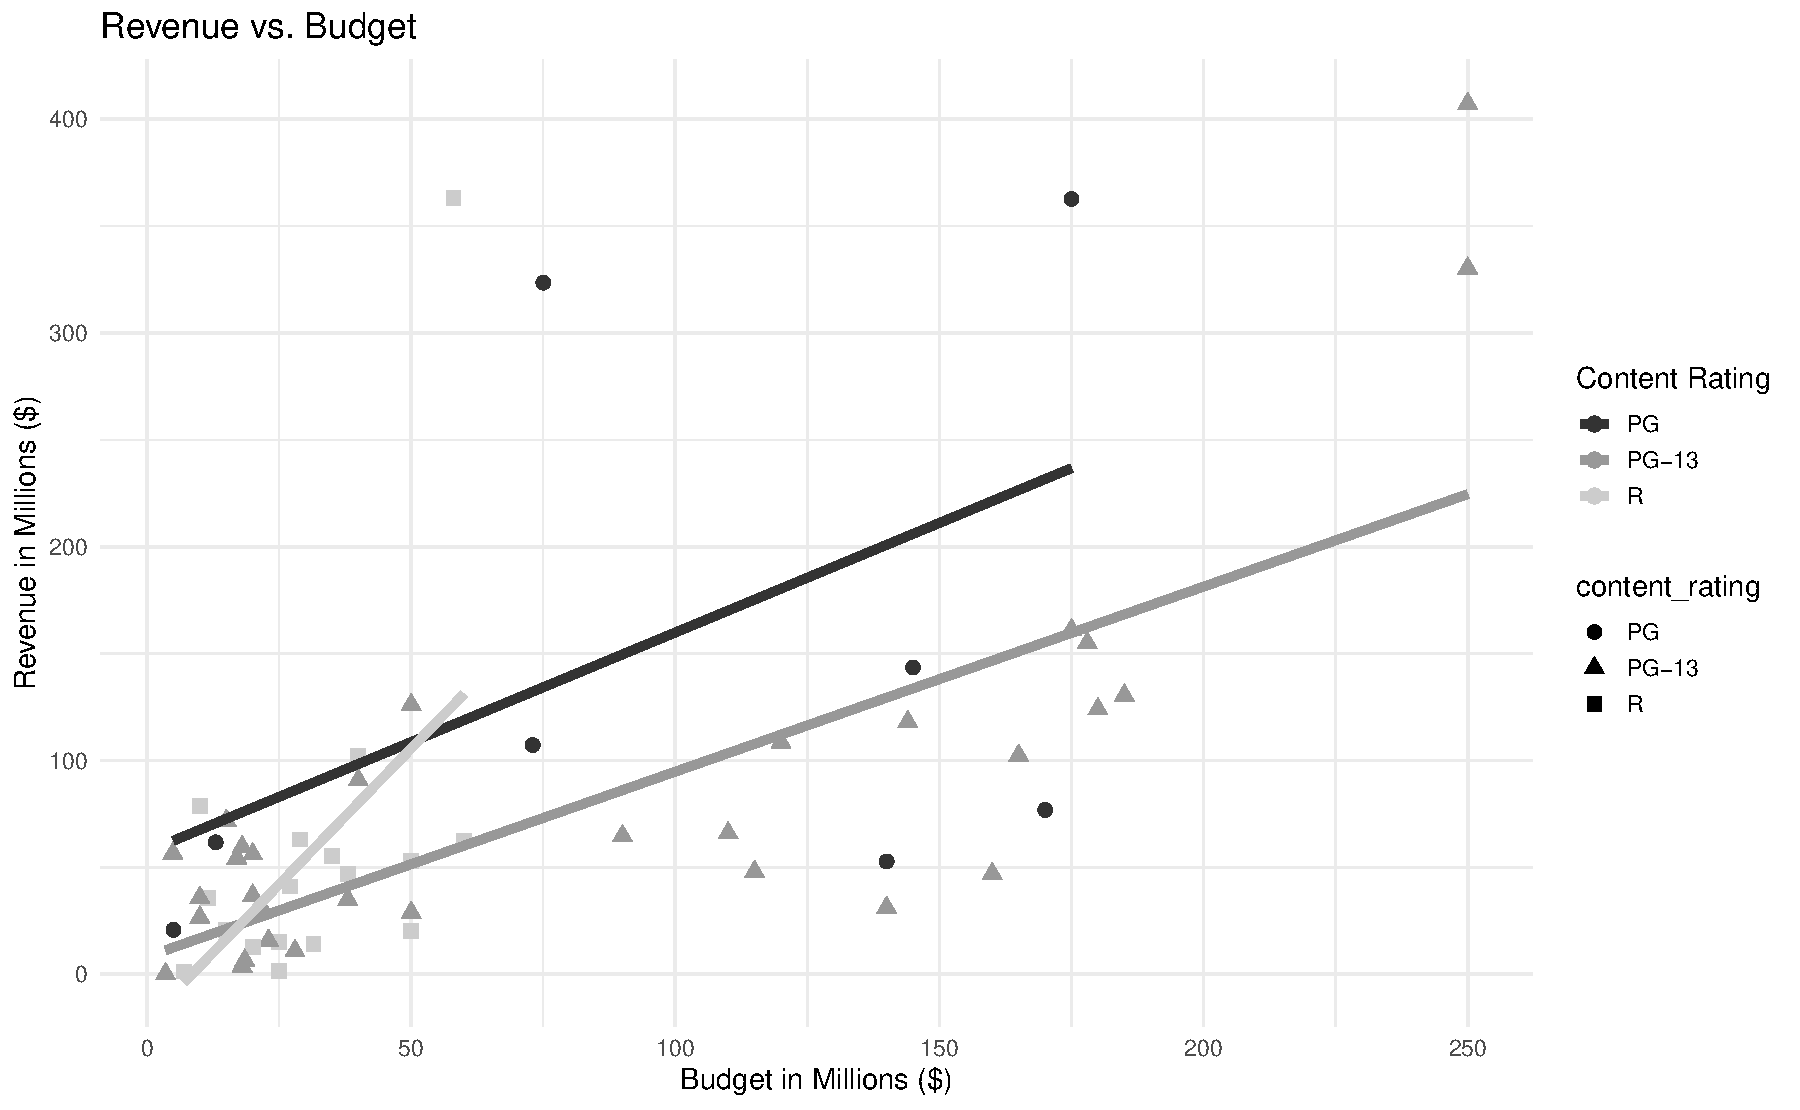
\includegraphics[width=0.7\linewidth]{05-EDA-multivariate_files/figure-latex/unnamed-chunk-5-1} \end{center}

\begin{enumerate}
\def\labelenumi{\arabic{enumi}.}
\setcounter{enumi}{3}
\tightlist
\item
  Identify the three variables plotted in this graph.
\end{enumerate}

\vspace{0.5in}

\begin{enumerate}
\def\labelenumi{\arabic{enumi}.}
\setcounter{enumi}{4}
\tightlist
\item
  Does the relationship between \texttt{Budget} and \texttt{Revenue} differ among the different content ratings? Explain.
\end{enumerate}

\vspace{1in}

\newpage

\hypertarget{additional-notes}{%
\section{Additional notes}\label{additional-notes}}

Use this space to summarize your thoughts and take additional notes on this week's activity and material covered.

\hypertarget{activity-6-handedness-of-male-boxers---testing}{%
\chapter{Activity 6: Handedness of Male Boxers - Testing}\label{activity-6-handedness-of-male-boxers---testing}}

\hypertarget{learning-objectives}{%
\section{Learning objectives}\label{learning-objectives}}

\begin{itemize}
\item
  Identify the two possible explanations (one assuming the null hypothesis, and one assuming the alternative hypothesis) for a relationship seen in sample data
\item
  Given a research question, construct the null and alternative hypotheses
  in words and using appropriate statistical symbols
\item
  Describe and perform simulation-based hypothesis tests for a single proportion
\item
  Interpret and evaluate a p-value
\end{itemize}

\hypertarget{terminology-review}{%
\section{Terminology review}\label{terminology-review}}

In this week's in-class activity, we will introduce simulation hypothesis testing for a single categorical variable. Some terms covered in this activity are:

\begin{itemize}
\item
  Parameter of interest
\item
  Null hypothesis
\item
  Alternative hypothesis
\item
  Simulation
\item
  Null distribution
\item
  p-value
\end{itemize}

To review these concepts, see Chapter 5 in your textbook, focusing on Sections 5.1 through 5.3.

\hypertarget{steps-of-the-statistical-investigation-process}{%
\section{Steps of the statistical investigation process}\label{steps-of-the-statistical-investigation-process}}

We will work through a six-step process to complete a hypothesis test for a single proportion.

\begin{itemize}
\item
  \textbf{Ask a research question} that can be addressed by collecting data. What are the researchers trying to show?
\item
  \textbf{Design a study and collect data}. This step involves selecting the people or objects to be studied and how to gather relevant data on them.
\item
  \textbf{Summarize and visualize the data}. Calculate summary statistics and create graphical plots that best represent the research question.
\item
  \textbf{Use statistical analysis methods to draw inferences from the data}. Choose an analysis technique appropriate for the data and identify the p-value. In this study, we will focus on using randomization.
\item
  \textbf{Communicate the results and answer the research question}. Using the p-value and confidence interval from the analysis, determine whether the data provide statistical evidence against the null hypothesis.
\item
  \textbf{Revisit and look forward} to point out limitations of the study and suggest new studies that could be performed to build on the findings of the study
\end{itemize}

\hypertarget{handedness-of-male-boxers}{%
\section{Handedness of male boxers}\label{handedness-of-male-boxers}}

Left-handedness is a trait that is found in about 10\% of the population. Past studies have shown that left-handed men are over-represented among professional boxers. The fighting claim states that left-handed men have an advantage in competition. In this random sample of 500 male professional boxers we want to see if there is an over-prevalence of left-handed fighters.

\hypertarget{summary-statistics-review-complete-q1---4-before-class}{%
\subsection*{Summary statistics review: Complete Q1 - 4 before class}\label{summary-statistics-review-complete-q1---4-before-class}}
\addcontentsline{toc}{subsection}{Summary statistics review: Complete Q1 - 4 before class}

\begin{enumerate}
\def\labelenumi{\arabic{enumi}.}
\tightlist
\item
  What are the observational units?
\end{enumerate}

\vspace{0.5in}

\begin{enumerate}
\def\labelenumi{\arabic{enumi}.}
\setcounter{enumi}{1}
\tightlist
\item
  What variable are we testing? Is it categorical or quantitative?
\end{enumerate}

\vspace{0.5in}

\begin{enumerate}
\def\labelenumi{\arabic{enumi}.}
\setcounter{enumi}{2}
\tightlist
\item
  What type of plot would be appropriate to visually display the data?
\end{enumerate}

\vspace{0.5in}

\begin{enumerate}
\def\labelenumi{\arabic{enumi}.}
\setcounter{enumi}{3}
\tightlist
\item
  Write out in context the statistic we will calculate to summarize the data.
\end{enumerate}

\vspace{0.5in}

\hypertarget{ask-a-research-question}{%
\subsection*{Ask a research question}\label{ask-a-research-question}}
\addcontentsline{toc}{subsection}{Ask a research question}

\begin{enumerate}
\def\labelenumi{\arabic{enumi}.}
\setcounter{enumi}{4}
\tightlist
\item
  Identify the research question for this study.
\end{enumerate}

\vspace{1in}

\hypertarget{design-a-study-and-collect-data}{%
\subsection*{Design a study and collect data}\label{design-a-study-and-collect-data}}
\addcontentsline{toc}{subsection}{Design a study and collect data}

Before completing the hypothesis test, we must check that the cases are independent. The sample observations are independent if the outcome of one observation does not influence the outcome of another. One way this condition is met is if data come from a simple random sample of the target population.

\begin{enumerate}
\def\labelenumi{\arabic{enumi}.}
\setcounter{enumi}{5}
\tightlist
\item
  Are the cases independent? Justify your answer.
\end{enumerate}

\vspace{1in}

\hypertarget{summarize-and-visualize-the-data}{%
\subsection*{Summarize and visualize the data}\label{summarize-and-visualize-the-data}}
\addcontentsline{toc}{subsection}{Summarize and visualize the data}

\begin{Shaded}
\begin{Highlighting}[]
\NormalTok{handedness \textless{}{-}}\StringTok{ }\KeywordTok{read.csv}\NormalTok{(}\StringTok{"data/Male\_boxers\_sample.csv"}\NormalTok{) }\CommentTok{\# Read in data set}
\NormalTok{handedness }\OperatorTok{\%\textgreater{}\%}\StringTok{ }\KeywordTok{count}\NormalTok{(Stance)  }\CommentTok{\# Count number in each Stance category}
\end{Highlighting}
\end{Shaded}

\begin{verbatim}
#>         Stance   n
#> 1  left-handed  81
#> 2 right-handed 419
\end{verbatim}

\begin{enumerate}
\def\labelenumi{\arabic{enumi}.}
\setcounter{enumi}{6}
\tightlist
\item
  Using the output above, calculate the appropriate summary statistic to represent the research question. Use appropriate notation.
\end{enumerate}

\vspace{0.5in}

\hypertarget{use-statistical-analysis-methods-to-draw-inferences-from-the-data}{%
\subsection*{Use statistical analysis methods to draw inferences from the data}\label{use-statistical-analysis-methods-to-draw-inferences-from-the-data}}
\addcontentsline{toc}{subsection}{Use statistical analysis methods to draw inferences from the data}

When testing data we must first identify the null hypothesis. The null hypothesis is written about the parameter of interest, or the true value of interest. \emph{For example, in the Martian Alphabet Activity the parameter of interest is the true proportion of statistic students who correctly identify Bumba.}

\begin{enumerate}
\def\labelenumi{\arabic{enumi}.}
\setcounter{enumi}{7}
\tightlist
\item
  Write out the parameter of interest for this study.
\end{enumerate}

\vspace{0.8in}

\begin{enumerate}
\def\labelenumi{\arabic{enumi}.}
\setcounter{enumi}{8}
\tightlist
\item
  Using the parameter of interest in question 8, write out the null hypothesis in words. What do we assume to be true about the parameter of interest?
\end{enumerate}

\newpage

The notation used for a true proportion is \(\pi\). Since this summarizes a population, it is a parameter. When writing the \textbf{null hypothesis} in notation we set the parameter equal to the null value, \(H_0: \pi = \pi_0\)

\begin{enumerate}
\def\labelenumi{\arabic{enumi}.}
\setcounter{enumi}{9}
\tightlist
\item
  Write the null hypothesis in notation using the null value of 0.1 in place of \(\pi_0\) in the equation given above.
\end{enumerate}

\vspace{0.5in}

The \textbf{alternative hypothesis} is the claim to be tested and the direction is based on the research question.

\begin{enumerate}
\def\labelenumi{\arabic{enumi}.}
\setcounter{enumi}{10}
\tightlist
\item
  Based on the research question from question 5, are we testing that the parameter is greater than 0.1, less than 0.1 or different than 0.1?
\end{enumerate}

\vspace{0.5in}

\begin{enumerate}
\def\labelenumi{\arabic{enumi}.}
\setcounter{enumi}{11}
\tightlist
\item
  Write out the alternative hypothesis in words.
\end{enumerate}

\vspace{1in}

\begin{enumerate}
\def\labelenumi{\arabic{enumi}.}
\setcounter{enumi}{12}
\tightlist
\item
  Write out the alternative hypothesis in notation.
\end{enumerate}

\vspace{0.5in}

Remember that when utilizing a hypothesis test, we are evaluating two competing possibilities. For this study the \textbf{two possibilities} are either\ldots{}

\begin{itemize}
\item
  The true proportion of male boxers who are left handed is 0.1 and our results just occurred by random chance or
\item
  The true proportion of male boxers who are left handed is greater than 0.1 and our results reflect this
\end{itemize}

Notice that these two competing possibilities represent the null and alternative hypotheses.

The null distribution is created under the assumption the null hypothesis is true. In this case, we assume the true proportion of male boxers who are left handed is 0.1 so we will create 1000 different simulations of 500 boxers under this assumption.

\newpage

Let's think about how to use red and blue cards to create one simulation of 500 boxers under the assumption the null hypothesis is true. Suppose blue cards represents left-handed and red cards represents right-handed.

\begin{enumerate}
\def\labelenumi{\arabic{enumi}.}
\setcounter{enumi}{13}
\tightlist
\item
  How many cards total do we need? How many blue ones? How many red ones?
\end{enumerate}

\vspace{0.5in}

\begin{enumerate}
\def\labelenumi{\arabic{enumi}.}
\setcounter{enumi}{14}
\tightlist
\item
  Next, we would mix the cards together and draw 1 card, write down if it's red or blue, and replace the card. How many times would we need to repeat this process to simulate our sample?
\end{enumerate}

\vspace{0.5in}

\begin{enumerate}
\def\labelenumi{\arabic{enumi}.}
\setcounter{enumi}{15}
\tightlist
\item
  Once we have one simulated sample, what would we calculate and plot on the null distribution? \emph{Hint}: What statistic are we calculating from the data?
\end{enumerate}

\vspace{1in}

We will use the computer to simulate a null distribution of 1000 different samples of 500 male boxers, plotting the proportion who are left handed in each sample, based on the assumption that the true proportion of male boxers who are left handed is 0.1 (or that the null hypothesis is true).

To use the computer simulation, we will need to enter the ``probability of success'' (\(\pi_0\)), ``sample size'' (the number of observational units or cases in the sample), ``number of repetitions'' (the number of samples to be generated), ``as extreme as'' (the observed statistic), and the ``direction'' (matches the direction of the alternative hypothesis).

\newpage

\begin{enumerate}
\def\labelenumi{\arabic{enumi}.}
\setcounter{enumi}{16}
\tightlist
\item
  What values should be entered for each of the following into the one proportion test to create 1000 simulations?
\end{enumerate}

\vspace{1mm}

\begin{itemize}
\tightlist
\item
  Probability of success:
\end{itemize}

\vspace{.2in}

\begin{itemize}
\tightlist
\item
  Sample size:
\end{itemize}

\vspace{.2in}

\begin{itemize}
\tightlist
\item
  Number of repetitions:
\end{itemize}

\vspace{.2in}

\begin{itemize}
\tightlist
\item
  As extreme as:
\end{itemize}

\vspace{.2in}

\begin{itemize}
\tightlist
\item
  Direction (\texttt{"greater"}, \texttt{"less"}, or \texttt{"two-sided"}):
\end{itemize}

\vspace{.2in}

Using the provided \texttt{RScript} file, fill in the values/words for xx with your answers from question 17 in the one proportion test to create a null distribution with 1000 simulations, highlight and run lines 1 - 14.

\begin{Shaded}
\begin{Highlighting}[]
\KeywordTok{one\_proportion\_test}\NormalTok{(}\DataTypeTok{probability\_success =}\NormalTok{ xx, }\CommentTok{\#Null hypothesis value}
                    \DataTypeTok{sample\_size =}\NormalTok{ xx, }\CommentTok{\#Enter sample size}
                    \DataTypeTok{number\_repetitions =} \DecValTok{1000}\NormalTok{, }\CommentTok{\#Enter number of simulations}
                    \DataTypeTok{as\_extreme\_as =}\NormalTok{ xx, }\CommentTok{\#observed statistic}
                    \DataTypeTok{direction =} \StringTok{"xx"}\NormalTok{, }\CommentTok{\#specify direction of alternative hypothesis}
                    \DataTypeTok{report\_value =} \StringTok{"proportion"}\NormalTok{) }\CommentTok{\#Reporting proportion or number of successes?}
\end{Highlighting}
\end{Shaded}

\begin{enumerate}
\def\labelenumi{\arabic{enumi}.}
\setcounter{enumi}{17}
\tightlist
\item
  Sketch the null distribution created from the R code here.
\end{enumerate}

\vspace{1.8in}

\begin{enumerate}
\def\labelenumi{\arabic{enumi}.}
\setcounter{enumi}{18}
\tightlist
\item
  Around what value is the null distribution centered? Why does that make sense?
\end{enumerate}

\vspace{1in}

\begin{enumerate}
\def\labelenumi{\arabic{enumi}.}
\setcounter{enumi}{19}
\tightlist
\item
  Circle the statistic (value from question 7) on the distribution you drew in question 18. Where does the statistic fall in the null distribution? Is it near the center of the distribution (near 0.1) or in one of the tails of the distribution?
\end{enumerate}

\vspace{1in}

\begin{enumerate}
\def\labelenumi{\arabic{enumi}.}
\setcounter{enumi}{20}
\tightlist
\item
  Is the statistic likely to happen or unlikely to happen if the true proportion of male boxers who are left-handed is 0.1? Explain your answer using the plot.
\end{enumerate}

\vspace{1in}

\begin{enumerate}
\def\labelenumi{\arabic{enumi}.}
\setcounter{enumi}{21}
\tightlist
\item
  Using the simulation, what is the proportion of simulated samples at the summary statistic or greater, if the true proportion of male boxers who are left-handed is 0.1? \emph{Hint}: Look under the simulation.
\end{enumerate}

\vspace{1in}

~~~~~~~~This is the \textbf{p-value}. The smaller the p-value the more evidence we have against the null hypothesis.

\begin{enumerate}
\def\labelenumi{\arabic{enumi}.}
\setcounter{enumi}{22}
\tightlist
\item
  Using the following guidelines for the strength of evidence, how much evidence do the data provide against the null hypothesis? (Circle one.)
\end{enumerate}

\begin{center}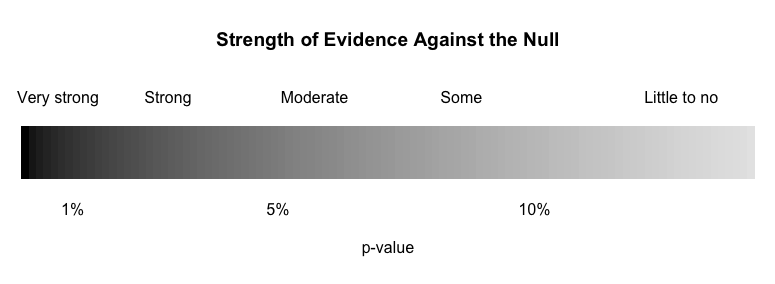
\includegraphics[width=0.9\linewidth]{images/soe_gradient_grayscale} \end{center}

\newpage

\begin{enumerate}
\def\labelenumi{\arabic{enumi}.}
\setcounter{enumi}{23}
\tightlist
\item
  What does the p-value measure? Interpret the p-value in context of the problem.
\end{enumerate}

\vspace{1in}

\hypertarget{communicate-the-results-and-answer-the-research-question}{%
\subsection*{Communicate the results and answer the research question}\label{communicate-the-results-and-answer-the-research-question}}
\addcontentsline{toc}{subsection}{Communicate the results and answer the research question}

When we write a conclusion we answer the research question by stating how much evidence there is for the alternative hypothesis.

\begin{enumerate}
\def\labelenumi{\arabic{enumi}.}
\setcounter{enumi}{24}
\tightlist
\item
  Write a conclusion in context of the study.
\end{enumerate}

\vspace{1in}

\begin{enumerate}
\def\labelenumi{\arabic{enumi}.}
\setcounter{enumi}{25}
\tightlist
\item
  Write a paragraph summarizing the results. Be sure to describe:
\end{enumerate}

\begin{itemize}
\item
  Summary statistic
\item
  P-value and interpretation
\item
  Conclusion (written to answer the research question)
\item
  Generalization - to what group do the results apply?
\end{itemize}

\vspace{3in}

\hypertarget{revisit-and-look-forward}{%
\subsection*{Revisit and look forward}\label{revisit-and-look-forward}}
\addcontentsline{toc}{subsection}{Revisit and look forward}

\begin{enumerate}
\def\labelenumi{\arabic{enumi}.}
\setcounter{enumi}{26}
\tightlist
\item
  Suggest a new research question that you might investigate, building on what you learned in this study.
\end{enumerate}

\vspace{.6in}

\hypertarget{out-of-class-activity}{%
\section{Out of Class Activity}\label{out-of-class-activity}}

The remaining questions cover theory-based methods for testing a single categorical variable. Use section 5.3.3 in the textbook and the OnePropTheory video to complete the following questions.

A single proportion can be mathematically modeled using the normal distribution if certain conditions are met.

Conditions for the sample distribution of \(\hat{p}\).

\begin{itemize}
\item
  Independence: The sample's observations are independent, e.g., are from a simple random sample
\item
  Success-Failure Condition: We \emph{expect} to see at least 10 successes and 10 failures in the sample, \(n\pi≥10\) and \(n(1-\pi)≥10\)
\end{itemize}

\begin{enumerate}
\def\labelenumi{\arabic{enumi}.}
\tightlist
\item
  We already verified that the independence condition is satisfied in question 6. Is the success-failure condition met to model the data with the Normal distribution? Show your work to support your answer.
\end{enumerate}

\vspace{1in}

To calculate the standardized statistic we use:

\[
Z = \frac{\text{point estimate} - \text{null value}}{SE}
\]
For a single categorical variable the standardized sample proportion is calculated using:

\[
Z = \frac{\hat{p} - \pi_0}{SE_0(\hat{p})}
\]
where the standard error is calculated using the null value.

\[SE_0(\hat{p})=\sqrt{\frac{\pi_0(1-\pi_0)}{n}}\]
\vspace{0.5mm}

\begin{enumerate}
\def\labelenumi{\arabic{enumi}.}
\setcounter{enumi}{1}
\tightlist
\item
  Calculate the null standard error of the sample proportion.
\end{enumerate}

\vspace{1in}

\begin{enumerate}
\def\labelenumi{\arabic{enumi}.}
\setcounter{enumi}{2}
\tightlist
\item
  Calculate the standardized sample proportion.
\end{enumerate}

\vspace{1in}

The standardized statistic is used as a ruler to measure how far the sample statistic is from the null value. Essentially we are converting the sample proportion into a measure of standard errors to compare to the standard normal distribution.

\begin{figure}

{\centering 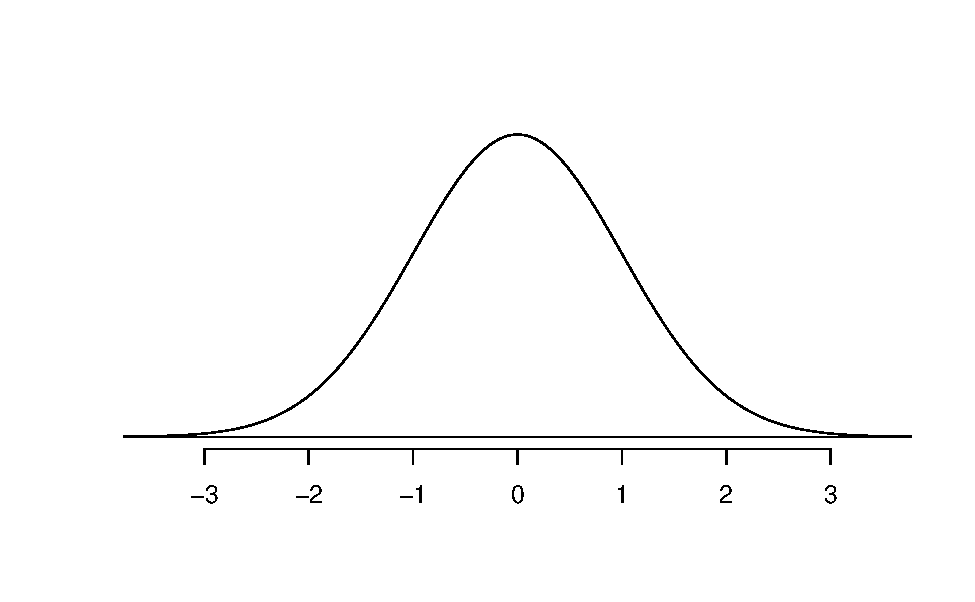
\includegraphics[width=0.7\linewidth]{06-inference-1cat_test_files/figure-latex/simpleNormal-1} 

}

\caption{A normal curve.}\label{fig:simpleNormal}
\end{figure}

\begin{enumerate}
\def\labelenumi{\arabic{enumi}.}
\setcounter{enumi}{3}
\tightlist
\item
  Using the 68-95-99.7 rule in Section 5.2.5 to guide you, mark on the standard normal distribution above the value of the standardized statistic calculated in question 3.
\end{enumerate}

\vspace{0.2in}

The standardized statistic measures the number of standard errors the sample statistic is from the null value.

\begin{enumerate}
\def\labelenumi{\arabic{enumi}.}
\setcounter{enumi}{4}
\tightlist
\item
  Interpret the standardized sample proportion from question 3 in context of the problem.
\end{enumerate}

\vspace{1in}

We will use the pnorm function in \texttt{R} to find the p-value. Use the provided \texttt{RScript} file and enter the value of the standardized statistic calculated in question 3 at xx in line 18, highlight and run lines 18 - 20. Notice that in line 20 it says \texttt{lower.tail\ =\ FALSE}. \texttt{R} will calculate the p-value greater than the value of the standardized statistic. Use \texttt{lower.tail\ =\ TRUE} when doing a left-sided test and \texttt{lower.tail\ =\ FALSE} when doing a right-sided test. To find a two-sided p-value use a left-sided test and multiply the p-value found by 2.

\begin{Shaded}
\begin{Highlighting}[]
\KeywordTok{pnorm}\NormalTok{(xx, }\CommentTok{\# Enter value of standardized statistic}
      \DataTypeTok{m=}\DecValTok{0}\NormalTok{, }\DataTypeTok{s=}\DecValTok{1} \CommentTok{\# Using the standard normal mean = 0, sd = 1}
      \DataTypeTok{lower.tail=}\OtherTok{FALSE}\NormalTok{) }\CommentTok{\# Gives a p{-}value greater than the standardized statistic}
\end{Highlighting}
\end{Shaded}

\begin{enumerate}
\def\labelenumi{\arabic{enumi}.}
\setcounter{enumi}{5}
\item
  Report the p-value obtained from the \texttt{R} output.
  \vspace{0.2in}
\item
  Is the p-value found in question 6 similar to the p-value found using the simulation test? Explain why you would expect this to be true.
\end{enumerate}

\vspace{0.5in}

\hypertarget{additional-notes}{%
\section{Additional notes}\label{additional-notes}}

Use this space to summarize your thoughts and take additional notes on this week's activity and material covered.

\hypertarget{activity-6-handedness-of-male-boxers---estimation}{%
\chapter{Activity 6: Handedness of Male Boxers - Estimation}\label{activity-6-handedness-of-male-boxers---estimation}}

\hypertarget{learning-objectives}{%
\section{Learning objectives}\label{learning-objectives}}

\begin{itemize}
\item
  Use bootstrapping to find a confidence interval for a single proportion
\item
  Interpret a confidence interval
\end{itemize}

\hypertarget{terminology-review}{%
\section{Terminology review}\label{terminology-review}}

In this week's in-class activity, we will introduce simulation confidence intervals for a single categorical variable. Some terms covered in this activity are:

\begin{itemize}
\item
  Parameter of interest
\item
  Bootstrapping
\item
  Confidence interval
\end{itemize}

To review these concepts, see Chapter 5 in your textbook, focusing on Sections 5.1 through 5.3.

\hypertarget{handedness-of-male-boxers}{%
\section{Handedness of male boxers}\label{handedness-of-male-boxers}}

Last week, we found very strong evidence that the true proportion of male boxers who are left-handed is greater than the general population, 0.1. We will use this same study to estimate the parameter of interest. As a reminder: left-handedness is a trait that is found in about 10\% of the population. Past studies have shown that left-handed men are over-represented among professional boxers. The fighting claim states that left-handed men have an advantage in competition. Using the data from this random sample of 500 male boxers we want to estimate the true proportion of male boxers who are left-handed. Recall from the last activity in the sample of 500 male boxers, 81 were left-handed.

A \textbf{point estimate} provides a single plausible value for a parameter. However, a point estimate is rarely perfect; usually there is some error in the estimate. In addition to supplying a point estimate of a parameter, a next logical step would be to provide a plausible range of values for the parameter. This plausible range of values for the population parameter is called a confidence interval.

\hypertarget{activity-intro.-complete-q1---4-before-class.}{%
\subsection*{Activity Intro. Complete Q1 - 4 before class.}\label{activity-intro.-complete-q1---4-before-class.}}
\addcontentsline{toc}{subsection}{Activity Intro. Complete Q1 - 4 before class.}

\begin{enumerate}
\def\labelenumi{\arabic{enumi}.}
\tightlist
\item
  What is the value of the point estimate?
\end{enumerate}

\vspace{0.5in}

\begin{enumerate}
\def\labelenumi{\arabic{enumi}.}
\setcounter{enumi}{1}
\tightlist
\item
  If we took another random sample of 500 male boxers, would you get the exact same point estimate? Explain why or why not.
\end{enumerate}

\vspace{0.5in}

In this week's activity, we will use bootstrapping to find the 95\% confidence interval. See Section 5.3.2 for more information on bootstrapping.

\begin{enumerate}
\def\labelenumi{\arabic{enumi}.}
\setcounter{enumi}{2}
\item
  In your own words, explain the bootstrapping process.
  \vspace{0.5in}
\item
  Write the conclusion to your test from activity 6.
\end{enumerate}

\vspace{0.5in}

\hypertarget{use-statistical-analysis-methods-to-draw-inferences-from-the-data}{%
\subsection*{Use statistical analysis methods to draw inferences from the data}\label{use-statistical-analysis-methods-to-draw-inferences-from-the-data}}
\addcontentsline{toc}{subsection}{Use statistical analysis methods to draw inferences from the data}

\begin{enumerate}
\def\labelenumi{\arabic{enumi}.}
\setcounter{enumi}{4}
\tightlist
\item
  Write out the parameter of interest for this study.
\end{enumerate}

\vspace{0.5in}

To use the computer simulation to create a bootstrap distribution, we will need to enter the ``sample size'' (the number of observational units or cases in the sample), ``number of successes'' (the number of cases that are left-handed), ``number of repetitions'' (the number of samples to be generated), and the ``confidence level'' (which level of confidence are we using to create the confidence interval).

\begin{enumerate}
\def\labelenumi{\arabic{enumi}.}
\setcounter{enumi}{5}
\tightlist
\item
  What values should be entered for each of the following into the simulation to create the bootstrap distribution to find a 95\% confidence interval?
  \vspace{1mm}
\end{enumerate}

\begin{itemize}
\tightlist
\item
  Sample size:
\end{itemize}

\vspace{.1in}

\begin{itemize}
\tightlist
\item
  Number of successes:
\end{itemize}

\vspace{.1in}

\begin{itemize}
\tightlist
\item
  Number of repetitions:
\end{itemize}

\vspace{.1in}

\begin{itemize}
\tightlist
\item
  Confidence level (as a decimal):
\end{itemize}

\vspace{.1in}

Using the provided \texttt{RScript} file, fill in the values/words for xx with your answers from question 6 in the one proportion bootstrap CI code to create a bootstrap distribution with 1000 simulations, highlight and run lines 1 - 11.

\begin{Shaded}
\begin{Highlighting}[]
\KeywordTok{one\_proportion\_bootstrap\_CI}\NormalTok{(}\DataTypeTok{sample\_size =}\NormalTok{ xx, }\CommentTok{\#Sample size}
                    \DataTypeTok{number\_successes =}\NormalTok{ xx, }\CommentTok{\#Observed number of successes}
                    \DataTypeTok{number\_repetitions =} \DecValTok{1000}\NormalTok{, }\CommentTok{\#Number of bootstrap samples to use}
                    \DataTypeTok{confidence\_level =} \FloatTok{0.95}\NormalTok{) }\CommentTok{\#Confidence level as a decimal}
\end{Highlighting}
\end{Shaded}

\begin{enumerate}
\def\labelenumi{\arabic{enumi}.}
\setcounter{enumi}{6}
\tightlist
\item
  Sketch the bootstrap distribution created below.
\end{enumerate}

\vspace{1.8in}

\begin{enumerate}
\def\labelenumi{\arabic{enumi}.}
\setcounter{enumi}{7}
\item
  What is the value at the center of this bootstrap distribution? Why does this make sense?
  \vspace{.8in}
\item
  Explain why the two vertical lines are at the 2.5th percentile and the 97.5th percentile.
\end{enumerate}

\vspace{.8in}

\begin{enumerate}
\def\labelenumi{\arabic{enumi}.}
\setcounter{enumi}{9}
\tightlist
\item
  Report the 95\% bootstrapped confidence interval for \(\pi\). Use interval notation: (lower value, upper value).
\end{enumerate}

\vspace{0.3in}

\begin{enumerate}
\def\labelenumi{\arabic{enumi}.}
\setcounter{enumi}{10}
\tightlist
\item
  Interpret the 95\% confidence interval in context.
\end{enumerate}

\vspace{.8in}

\hypertarget{communicate-the-results-and-answer-the-research-question}{%
\subsection*{Communicate the results and answer the research question}\label{communicate-the-results-and-answer-the-research-question}}
\addcontentsline{toc}{subsection}{Communicate the results and answer the research question}

\begin{enumerate}
\def\labelenumi{\arabic{enumi}.}
\setcounter{enumi}{11}
\tightlist
\item
  Does the confidence interval confirm your conclusion from activity 6? Explain your answer.
\end{enumerate}

\vspace{1in}

\newpage

\hypertarget{effect-of-confidence-level}{%
\subsection{Effect of confidence level}\label{effect-of-confidence-level}}

\begin{enumerate}
\def\labelenumi{\arabic{enumi}.}
\setcounter{enumi}{12}
\tightlist
\item
  Suppose instead of finding a 95\% confidence interval, we found a 90\% confidence interval. Would you expect the 90\% confidence interval to be narrower or wider? Explain your answer.
\end{enumerate}

\vspace{0.5in}

\begin{enumerate}
\def\labelenumi{\arabic{enumi}.}
\setcounter{enumi}{13}
\tightlist
\item
  The following \texttt{R} code produced the bootstrap distribution with 1000 simulations that follows. What value changed in the code?
\end{enumerate}

\begin{Shaded}
\begin{Highlighting}[]
\KeywordTok{one\_proportion\_bootstrap\_CI}\NormalTok{(}\DataTypeTok{sample\_size =} \DecValTok{500}\NormalTok{, }\CommentTok{\#Sample size}
                    \DataTypeTok{number\_successes =} \DecValTok{81}\NormalTok{, }\CommentTok{\#Observed number of successes}
                    \DataTypeTok{number\_repetitions =} \DecValTok{1000}\NormalTok{, }\CommentTok{\#Number of bootstrap samples to use}
                    \DataTypeTok{confidence\_level =} \FloatTok{0.90}\NormalTok{) }\CommentTok{\#Confidence level as a decimal}
\end{Highlighting}
\end{Shaded}

\begin{center}\includegraphics[width=0.7\linewidth]{07-inference-1cat_CI_files/figure-latex/unnamed-chunk-2-1} \end{center}

\vspace{0.5in}

\begin{enumerate}
\def\labelenumi{\arabic{enumi}.}
\setcounter{enumi}{14}
\tightlist
\item
  Report both the 95\% confidence interval (question 10) and the 90\% confidence interval (question 14). Is the 90\% confidence interval narrower or wider than the 95\% confidence interval?
\end{enumerate}

\vspace{0.5in}

\newpage

\hypertarget{what-does-confidence-mean}{%
\subsection{\texorpdfstring{What does \emph{confidence} mean?}{What does confidence mean?}}\label{what-does-confidence-mean}}

In the interpretation of the confidence interval, we say that we are 95\% or 90\% confident that the parameter is within the confidence interval. Why are we able to make that claim? What does it mean to say ``we are 95\% confident''?

\begin{enumerate}
\def\labelenumi{\arabic{enumi}.}
\setcounter{enumi}{15}
\tightlist
\item
  Go to this website, \url{http://www.rossmanchance.com/ISIapplets.html} and choose \texttt{Simulating\ Confidence\ Intervals}. In the input on the left-hand side of the screen enter 0.1 for \(\pi\), 500 for \(n\), and 100 for \texttt{Intervals}. Click 'sample`.
  \vspace{1mm}
\end{enumerate}

~~~In the graph on the bottom right, click on a green dot. Write down the confidence interval for this sample given on the graph on the left. Does this confidence interval contain the null value of 0.1?

\vspace{0.5in}

~~~Now click on a red dot. Write down the confidence interval for this sample. Does this confidence interval contain the null value of 0.1.?

\vspace{0.5in}

~~~How many intervals out of 100 contain \(\pi\), the null value of 0.1? \emph{Hint}: This is given to the left of the graph of green and red intervals.

\vspace{0.5in}

\begin{enumerate}
\def\labelenumi{\arabic{enumi}.}
\setcounter{enumi}{16}
\tightlist
\item
  Click on \texttt{sample} nine more times. Write down the \texttt{Running\ Total} for the proportion of intervals that contain \(\pi\).
\end{enumerate}

\vspace{0.5in}

\begin{enumerate}
\def\labelenumi{\arabic{enumi}.}
\setcounter{enumi}{17}
\tightlist
\item
  Interpret the level of confidence in context of the problem. \emph{Hint}: What proportion of samples would we expect to give a confidence interval that contains the parameter of interest?
\end{enumerate}

\vspace{1in}

\hypertarget{revisit-and-look-forward}{%
\subsection*{Revisit and look forward}\label{revisit-and-look-forward}}
\addcontentsline{toc}{subsection}{Revisit and look forward}

\begin{enumerate}
\def\labelenumi{\arabic{enumi}.}
\setcounter{enumi}{18}
\tightlist
\item
  Suggest a new research question that you might investigate, building on what you learned in this study.
\end{enumerate}

\vspace{.6in}

\newpage

\hypertarget{out-of-class-activity}{%
\section{Out of Class Activity}\label{out-of-class-activity}}

The remaining questions cover theory-based methods for testing a single categorical variable. Use section 5.3.3 in the textbook and the OnePropTheory video to complete the following questions.

Recall that to use theory-based methods we must check the conditions to approximate the sample distribution with the Normal distribution. From the previous activity we saw that independence was satisfied as the researchers took a random sample.

For finding a confidence interval we need to be sure we have at least 10 successes and 10 failures in our \textbf{sample}.

\begin{itemize}
\tightlist
\item
  \(n\hat{p}≥10\) and \(n(1-\hat{p})≥10\)
\end{itemize}

\begin{enumerate}
\def\labelenumi{\arabic{enumi}.}
\tightlist
\item
  Verify that the success/failure condition is met to use theory based methods to find a 95\% confidence interval.
\end{enumerate}

\vspace{0.5in}

To calculate the 95\% confidence interval we will find the standard error using the sample proportion.

\[SE(\hat{p}) = \sqrt{\frac{\hat{p}(1-\hat{p})}{n}}\]
To find the confidence interval we will add and subtract the margin of error to the point estimate.

\[\text{point estimate}\pm\text{margin of error}\]
\[\hat{p}\pm z^* SE(\hat{p})\]

\begin{enumerate}
\def\labelenumi{\arabic{enumi}.}
\setcounter{enumi}{1}
\tightlist
\item
  Calculate the standard error of the sample proportion to find a 95\% confidence interval.
\end{enumerate}

\vspace{0.5in}

The \(z^*\) multiplier is found under the standard normal distribution. We find the values that encompass the middle 95\% of the distribution. If 95\% of the standard normal distribution should be in the middle, that leaves 5\% in the tails, or 2.5\% in each tail. The qnorm function in \texttt{R} will tell us the \(z^*\) value for the desired percentile (in this case, 95\% + 2.5\% = 97.5\% percentile).

\begin{Shaded}
\begin{Highlighting}[]
\KeywordTok{qnorm}\NormalTok{(}\FloatTok{0.975}\NormalTok{) }\CommentTok{\# Multiplier for 95\% confidence interval}
\end{Highlighting}
\end{Shaded}

\begin{verbatim}
#> [1] 1.959964
\end{verbatim}

\begin{enumerate}
\def\labelenumi{\arabic{enumi}.}
\setcounter{enumi}{2}
\tightlist
\item
  Using the multiplier of \(z^*\) = 1.96, calculate the 95\% confidence interval for the true proportion of male boxers who are left-handed.
\end{enumerate}

\vspace{1in}

\begin{enumerate}
\def\labelenumi{\arabic{enumi}.}
\setcounter{enumi}{3}
\tightlist
\item
  Verify that the simulation confidence interval found using bootstrapping is similar to the confidence interval calculating using theory-based methods.
\end{enumerate}

\vspace{1in}

\hypertarget{additional-notes}{%
\section{Additional notes}\label{additional-notes}}

Use this space to summarize your thoughts and take additional notes on this week's activity and material covered.

\hypertarget{activity-8-winter-sports-helmet-use-and-head-injuries---testing}{%
\chapter{Activity 8: Winter Sports Helmet Use and Head Injuries - Testing}\label{activity-8-winter-sports-helmet-use-and-head-injuries---testing}}

\hypertarget{learning-objectives}{%
\section{Learning objectives}\label{learning-objectives}}

\begin{itemize}
\item
  Write out the null and alternative hypotheses for two categorical variables
\item
  Assess the conditions to use the standard normal distribution for a difference in proportions
\item
  Calculate the Z test statistic for the difference in proportions
\item
  Find the p-value and assess the strength of evidence
\end{itemize}

\hypertarget{terminology-review}{%
\section{Terminology review}\label{terminology-review}}

In this week's in-class activity, we will use theory-based methods to analyze two categorical variables. Some terms covered in this activity are:

\begin{itemize}
\item
  Conditional proportion
\item
  Z test
\item
  \(z*\) multiplier
\item
  Null hypothesis
\item
  Alternative hypothesis
\item
  Test statistic
\item
  Standard normal distribution
\item
  Independence and success-failure conditions
\item
  Type 1 and Type 2 errors
\item
  Decisions
\end{itemize}

To review these concepts, see Chapter 5 in your textbook.

\newpage

\hypertarget{helmet-use-and-head-injuries}{%
\section{Helmet use and head injuries}\label{helmet-use-and-head-injuries}}

In ``Helmet Use and Risk of Head Injuries in Alpine Skiers and Snowboarders'' by Sullheim et. al., in the \emph{Journal of the American Medical Association}, Vol. 295, No.~8 (2006), we can see the summary results from a random sample of 3562 skiers and snowboarders involved in accidents in the two-way table below. Is there evidence that safety helmet use is associated with a reduced risk of head injury for skiers and snowboarders?

\begin{longtable}[]{@{}cccc@{}}
\toprule
& Helmet Use & No Helmet Use & Total\tabularnewline
\midrule
\endhead
Head Injury & 96 & 480 & 576\tabularnewline
No Head Injury & 656 & 2330 & 2986\tabularnewline
Total & 752 & 2810 & 3562\tabularnewline
\bottomrule
\end{longtable}

These counts can be found in \texttt{R} by using the \texttt{count()} function:

\begin{Shaded}
\begin{Highlighting}[]
\NormalTok{injury \textless{}{-}}\StringTok{ }\KeywordTok{read.csv}\NormalTok{(}\StringTok{"https://math.montana.edu/courses/s216/data/HeadInjuries.csv"}\NormalTok{) }\CommentTok{\# Read data set in}
\NormalTok{injury \textless{}{-}}\StringTok{ }\CommentTok{\# Write over original data with the following}
\StringTok{  }\NormalTok{injury }\OperatorTok{\%\textgreater{}\%}\StringTok{ }\CommentTok{\# Pipe data set into}
\StringTok{  }\KeywordTok{mutate}\NormalTok{(Helmet \textless{}{-}}\StringTok{ }\KeywordTok{factor}\NormalTok{(Helmet),}
\NormalTok{         Outcome \textless{}{-}}\StringTok{ }\KeywordTok{factor}\NormalTok{(Outcome)) }\CommentTok{\# Convert to factors}

\NormalTok{injury }\OperatorTok{\%\textgreater{}\%}\StringTok{ }\KeywordTok{group\_by}\NormalTok{(Helmet) }\OperatorTok{\%\textgreater{}\%}\StringTok{ }\KeywordTok{count}\NormalTok{(Outcome)}
\end{Highlighting}
\end{Shaded}

\begin{verbatim}
#> # A tibble: 4 x 3
#> # Groups:   Helmet [2]
#>   Helmet Outcome            n
#>   <chr>  <chr>          <int>
#> 1 No     Head Injury      480
#> 2 No     No Head Injury  2330
#> 3 Yes    Head Injury       96
#> 4 Yes    No Head Injury   656
\end{verbatim}

Notice that the name of the explanatory variable is \texttt{Helmet} with outcomes \texttt{Yes} and \texttt{No} and the name of the response variable is \texttt{Outcome} with outcomes \texttt{Head\ Injury} and \texttt{No\ Head\ Injury}.

\hypertarget{vocabulary-review.-complete-q1---4-before-class.}{%
\subsection*{Vocabulary review. Complete Q1 - 4 before class.}\label{vocabulary-review.-complete-q1---4-before-class.}}
\addcontentsline{toc}{subsection}{Vocabulary review. Complete Q1 - 4 before class.}

\begin{enumerate}
\def\labelenumi{\arabic{enumi}.}
\tightlist
\item
  What is the explanatory variable?
\end{enumerate}

\vspace{0.3in}

\begin{enumerate}
\def\labelenumi{\arabic{enumi}.}
\setcounter{enumi}{1}
\tightlist
\item
  What is the response variable?
\end{enumerate}

\vspace{0.3in}

\begin{enumerate}
\def\labelenumi{\arabic{enumi}.}
\setcounter{enumi}{2}
\tightlist
\item
  Is this an experiment or observational study? Justify your answer.
\end{enumerate}

\newpage

\begin{enumerate}
\def\labelenumi{\arabic{enumi}.}
\setcounter{enumi}{3}
\tightlist
\item
  Put an X in the box that represents the appropriate scope of inference for this study.
\end{enumerate}

\begin{longtable}[]{@{}cccl@{}}
\toprule
& & Study Type &\tabularnewline
\midrule
\endhead
& & Randomized Experiment & Observational Study\tabularnewline
Selection of Cases & Random Sample & &\tabularnewline
& No Random Sample & &\tabularnewline
\bottomrule
\end{longtable}

\hypertarget{ask-a-research-question}{%
\subsection*{Ask a research question}\label{ask-a-research-question}}
\addcontentsline{toc}{subsection}{Ask a research question}

In this study we are looking at the relationship between two groups or two parameters (\(\pi_1\) and \(\pi_2\)). Remember we define the parameter for a categorical variable as the true proportion of observational units that are labeled as a ``success'' in the response variable.

\begin{enumerate}
\def\labelenumi{\arabic{enumi}.}
\setcounter{enumi}{4}
\item
  Write the two parameters of interest for this study. Let 1 = skier/snowboarder wore helmet, 2 = skier/snowboarder did not wear helmet.
  \vspace{1mm}

  \(\pi_1\) -
  \vspace{0.5in}

  \(\pi_2\) -
  \vspace{0.5in}
\end{enumerate}

When comparing two groups, we assume the two parameters are equal in the null hypothesis---there is no association between the variables.

\begin{enumerate}
\def\labelenumi{\arabic{enumi}.}
\setcounter{enumi}{5}
\tightlist
\item
  Write the null hypothesis out in words using your answers to question 5.
\end{enumerate}

\vspace{0.81in}

\begin{enumerate}
\def\labelenumi{\arabic{enumi}.}
\setcounter{enumi}{6}
\tightlist
\item
  What is the research question?
\end{enumerate}

\vspace{0.5in}

\begin{enumerate}
\def\labelenumi{\arabic{enumi}.}
\setcounter{enumi}{7}
\tightlist
\item
  Based on the research question fill in the appropriate sign for the alternative hypothesis (\(<\), \(>\), or \(\neq\)):
  \vspace{0.25in}
\end{enumerate}

~~~~~~~~~~\(H_A: \pi_1 -\pi_2\) \_\_\_\_\_\_\_\_\_\_ 0

\newpage

\hypertarget{summarize-and-visualize-the-data}{%
\subsection*{Summarize and visualize the data}\label{summarize-and-visualize-the-data}}
\addcontentsline{toc}{subsection}{Summarize and visualize the data}

\begin{enumerate}
\def\labelenumi{\arabic{enumi}.}
\setcounter{enumi}{8}
\tightlist
\item
  Using the two-way table, calculate the conditional proportion of skiers/snowboarders that wore a helmet with a head injury.
\end{enumerate}

\vspace{.3in}

\begin{enumerate}
\def\labelenumi{\arabic{enumi}.}
\setcounter{enumi}{9}
\tightlist
\item
  Using the two-way table, calculate the conditional proportion of skiers/snowboarders that did not wear a helmet with a head injury.
\end{enumerate}

\vspace{.3in}

\begin{center}\includegraphics[width=0.7\linewidth]{08-inference-2cat_test_files/figure-latex/unnamed-chunk-2-1} \end{center}

\begin{enumerate}
\def\labelenumi{\arabic{enumi}.}
\setcounter{enumi}{10}
\tightlist
\item
  Fill in the blanks on the graph above with the appropriate variables and values to complete the segmented bar plot showing the proportion of head injuries between those who wear helmets and those who do not wear helmets. \emph{Hint}: Use the conditional proportions from questions 9 and 10.
\end{enumerate}

\vspace{1mm}

\begin{enumerate}
\def\labelenumi{\arabic{enumi}.}
\setcounter{enumi}{11}
\tightlist
\item
  Based on the segmented bar plot, Does there appear to be an association between helmet use and head injury? Explain using the plot.
\end{enumerate}

\vspace{0.7in}

\begin{enumerate}
\def\labelenumi{\arabic{enumi}.}
\setcounter{enumi}{12}
\tightlist
\item
  Calculate the summary statistic for this study. Use helmet use (\texttt{Yes}) minus no helmet use (\texttt{No}) as the order of subtraction.
\end{enumerate}

\vspace{0.5in}

\begin{enumerate}
\def\labelenumi{\arabic{enumi}.}
\setcounter{enumi}{13}
\tightlist
\item
  What is the notation used for the value calculated in question 13?
\end{enumerate}

\vspace{0.2in}
\newpage

\hypertarget{use-statistical-analysis-methods-to-draw-inferences-from-the-data}{%
\subsection*{Use statistical analysis methods to draw inferences from the data}\label{use-statistical-analysis-methods-to-draw-inferences-from-the-data}}
\addcontentsline{toc}{subsection}{Use statistical analysis methods to draw inferences from the data}

To test the null hypothesis we could use simulation methods as we did with a single categorical variable in class. In this in-class activity we will focus on theory-based methods. Like with a single proportion, the difference in proportions can be mathematically modeled using the normal distribution if certain conditions are met.

Conditions for the sample distribution of \(\hat{p}_1-\hat{p}_2\):

\begin{itemize}
\item
  Independence: The data are independent within and between the two groups. (\emph{Remember}: This also must be true to use simulation methods!)
\item
  Success-Failure Condition: The success-failure condition holds for each group. Under the null hypothesis, the proportions \(\pi_1\) and \(\pi_2\) are equal, so we check the success-failure condition with our best estimate of these values under \(H_0\), the pooled proportion from the two samples,
\end{itemize}

\[
\hat{p}_{pool} = \frac{\text{number of "successes"}}{\text{number of cases}} = \frac{\hat{p}_1 n_1+\hat{p}_2 n_2}{n_1+n_2}
\]

~~~~\[\hat{p}_{pool} * n_1 \ge 10, (1 - \hat{p}_{pool}) * n_1 \ge 10\]\\
\hspace*{0.333em}\hspace*{0.333em}\hspace*{0.333em}\hspace*{0.333em}\[\hat{p}_{pool} * n_2 \ge 10, (1 - \hat{p}_{pool}) * n_2 \ge 10\]

\vspace{.25in}

\begin{enumerate}
\def\labelenumi{\arabic{enumi}.}
\setcounter{enumi}{14}
\tightlist
\item
  Is the independence condition met? Explain your answer.
\end{enumerate}

\vspace{0.5in}

\begin{enumerate}
\def\labelenumi{\arabic{enumi}.}
\setcounter{enumi}{15}
\tightlist
\item
  Is the success-failure condition met for each group? Show your work to verify your answer.
\end{enumerate}

\vspace{1in}

To calculate the standardized statistic we use:

\[
Z = \frac{\text{point estimate} - \text{null value}}{SE}
\]

where the null standard error is calculated using the pooled proportion of successes.

\[
SE_0(\hat{p}_1-\hat{p}_2)=\sqrt{\hat{p}_{pool}(1-\hat{p}_{pool})(\frac{1}{n_1}+\frac{1}{n_2})}
\]

\vspace{.25in}

\begin{enumerate}
\def\labelenumi{\arabic{enumi}.}
\setcounter{enumi}{16}
\tightlist
\item
  Calculate the \(SE_0(\hat{p}_1-\hat{p}_2)\).
\end{enumerate}

\vspace{1in}

\begin{enumerate}
\def\labelenumi{\arabic{enumi}.}
\setcounter{enumi}{17}
\tightlist
\item
  Calculate the standardized statistic.
\end{enumerate}

\vspace{1in}

We will use the pnorm function in \texttt{R} to find the p-value. Use the provided \texttt{RScript} file and enter the value of the standardized statistic found in question 18 at xx in line 27, highlight and run lines 27 - 29.

\begin{Shaded}
\begin{Highlighting}[]
\KeywordTok{pnorm}\NormalTok{(xx, }\CommentTok{\# Enter value of standardized statistic}
      \DataTypeTok{m=}\DecValTok{0}\NormalTok{, }\DataTypeTok{s=}\DecValTok{1} \CommentTok{\# Using the standard normal mean = 0, sd = 1}
      \DataTypeTok{lower.tail=}\OtherTok{TRUE}\NormalTok{) }\CommentTok{\# Gives a p{-}value less than the standardized statistic}
\end{Highlighting}
\end{Shaded}

\begin{enumerate}
\def\labelenumi{\arabic{enumi}.}
\setcounter{enumi}{18}
\item
  Report the p-value from the \texttt{R} output.
  \vspace{0.2in}
\item
  Interpret the p-value in context of the study.
\end{enumerate}

\vspace{1in}

\begin{enumerate}
\def\labelenumi{\arabic{enumi}.}
\setcounter{enumi}{20}
\tightlist
\item
  How much evidence does the p-value provide against the null hypothesis? \emph{Hint}: Refer to the guidelines given in activity 6.
\end{enumerate}

\vspace{0.4in}

\begin{enumerate}
\def\labelenumi{\arabic{enumi}.}
\setcounter{enumi}{21}
\tightlist
\item
  Write a conclusion to the test.
\end{enumerate}

\vspace{1in}

\hypertarget{types-of-errors}{%
\subsection*{Types of errors}\label{types-of-errors}}
\addcontentsline{toc}{subsection}{Types of errors}

Hypothesis tests are not flawless. In a hypothesis test, there are two competing hypotheses: the null and alternative. We make a decision about which might be true, but we may choose incorrectly.

\begin{table}
\caption{Four different possible scenarios for hypothesis tests.}
\centering
\begin{tabular}[h]{ll|cc}
\hline
 & &  \multicolumn{2}{c}{\textbf{Test conclusion}} \\
 &  & \multicolumn{1}{c}{Fail to reject $H_0$} & \multicolumn{1}{c}{Reject $H_0$}\\
\hline
 & $H_0$ true & Good decision & Type 1 Error\\
\hline
\textbf{Truth} & $H_A$ true & Type 2 Error & Good decision\\
\hline
\end{tabular}
\end{table}

Shown in the table above, a \textbf{Type 1 Error} is rejecting the null hypothesis when \(H_0\) is actually true. A \textbf{Type 2 Error} is failing to reject the null hypothesis when the alternative is actually true.

\begin{enumerate}
\def\labelenumi{\arabic{enumi}.}
\setcounter{enumi}{22}
\tightlist
\item
  Using a significance level of 0.05, based on the p-value found in question 19, what decision do you make in regards to the null hypothesis?
\end{enumerate}

\vspace{0.5in}

\begin{enumerate}
\def\labelenumi{\arabic{enumi}.}
\setcounter{enumi}{23}
\tightlist
\item
  What type of error could we have made?
\end{enumerate}

\vspace{0.5in}

\begin{enumerate}
\def\labelenumi{\arabic{enumi}.}
\setcounter{enumi}{24}
\tightlist
\item
  Write this error in context of the problem.
\end{enumerate}

\vspace{1in}

\begin{enumerate}
\def\labelenumi{\arabic{enumi}.}
\setcounter{enumi}{25}
\tightlist
\item
  Write a paragraph summarizing the results of the study. Be sure to describe:
\end{enumerate}

\begin{itemize}
\item
  Summary statistic
\item
  Test statistic and interpretation
\item
  P-value and interpretation
\item
  Conclusion (written to answer the research question)
\item
  Scope of inference
\end{itemize}

\vspace{2in}

\newpage

\hypertarget{out-of-class-activity}{%
\section{Out of Class Activity}\label{out-of-class-activity}}

The remaining questions cover simulation methods for testing two categorical variables. Use section 5.4.3 in the textbook and the TwoPropSim video to complete the following questions.

\begin{enumerate}
\def\labelenumi{\arabic{enumi}.}
\item
  First let's think about how one simulation would be created on the null distribution using cards.

  How many cards would you need?
  \vspace{0.1in}

  What would be written on each card?
\end{enumerate}

\vspace{0.5in}

\begin{enumerate}
\def\labelenumi{\arabic{enumi}.}
\setcounter{enumi}{1}
\tightlist
\item
  Next, we would mix the cards together and shuffle into two piles. How many cards would be in each pile? What would each pile represent?
\end{enumerate}

\vspace{1in}

\begin{enumerate}
\def\labelenumi{\arabic{enumi}.}
\setcounter{enumi}{2}
\tightlist
\item
  Once we have one simulated sample, what would we calculate and plot on the null distribution? \emph{Hint}: What statistic are we calculating from the data?
\end{enumerate}

\vspace{1in}

To create the null distribution, we will use the two proportion test. We will need to enter the response variable name and the explanatory variable name for the formula, the data set name identified above as \texttt{injury}, the outcome for the explanatory variable to give the order of subtraction for First in Subtraction, number of repetitions, the outcome for the response variable that is a success for Response Value Numerator, and the direction of the alternative hypothesis.

The response variable name is Outcome and the explanatory variable name is Helmet.

\newpage

\begin{enumerate}
\def\labelenumi{\arabic{enumi}.}
\setcounter{enumi}{3}
\tightlist
\item
  What inputs should be entered for each of the following to create the simulation?
\end{enumerate}

\vspace{.2in}

\begin{itemize}
\tightlist
\item
  First in Subtraction (What is the outcome for the explanatory variable that is used as first in the order of subtraction? \texttt{"Yes"} or \texttt{"No"}):
\end{itemize}

\vspace{.2in}

\begin{itemize}
\tightlist
\item
  Number of repetitions:
\end{itemize}

\vspace{.2in}

\begin{itemize}
\tightlist
\item
  Response Value Numerator (What is the outcome for the response variable that is considered a success? \texttt{"Head\ Injury"} or \texttt{"No\ Head\ Injury"}):
\end{itemize}

\vspace{.2in}

\begin{itemize}
\tightlist
\item
  As extreme as (enter the value for the sample difference in proportions):
\end{itemize}

\vspace{.2in}

\begin{itemize}
\tightlist
\item
  Direction (\texttt{"greater"}, \texttt{"less"}, or \texttt{"two-sided"}):
\end{itemize}

\vspace{.2in}

Using the \texttt{RScript} file for this activity, enter your answers for question 4 in place of the xx's in the two proportion test code to produce the null distribution with 1000 simulations, highlight and run lines 1 - 12 and then 33 - 39.

\begin{Shaded}
\begin{Highlighting}[]
\KeywordTok{two\_proportion\_test}\NormalTok{(}\DataTypeTok{formula =}\NormalTok{ Outcome }\OperatorTok{\textasciitilde{}}\StringTok{ }\NormalTok{Helmet, }\CommentTok{\#response\textasciitilde{}explanatory}
                    \DataTypeTok{data=}\NormalTok{ injury, }\CommentTok{\#name of dataset}
                    \DataTypeTok{first\_in\_subtraction =} \StringTok{"xx"}\NormalTok{, }\CommentTok{\#order of subtraction: enter the name of Group 1}
                    \DataTypeTok{number\_repetitions =} \DecValTok{1000}\NormalTok{, }\CommentTok{\#always use a minimum of 1000 repetitions}
                    \DataTypeTok{response\_value\_numerator =} \StringTok{"xx"}\NormalTok{, }\CommentTok{\#define which outcome is a success }
                    \DataTypeTok{as\_extreme\_as =}\NormalTok{ xx, }\CommentTok{\#type your calculated observed statistic (difference in sample proportions)}
                    \DataTypeTok{direction=}\StringTok{"xx"}\NormalTok{) }\CommentTok{\#alternative hypothesis direction ("greater","less","two{-}sided")}
\end{Highlighting}
\end{Shaded}

\begin{enumerate}
\def\labelenumi{\arabic{enumi}.}
\setcounter{enumi}{4}
\tightlist
\item
  Sketch the null distribution created here.
\end{enumerate}

\newpage

\begin{enumerate}
\def\labelenumi{\arabic{enumi}.}
\setcounter{enumi}{5}
\tightlist
\item
  What value is the null distribution centered around? Explain why this makes sense?
\end{enumerate}

\vspace{1in}

\begin{enumerate}
\def\labelenumi{\arabic{enumi}.}
\setcounter{enumi}{6}
\tightlist
\item
  What is the p-value? \emph{Remember}: This is the value given at the bottom of the null distribution.
\end{enumerate}

\vspace{0.2in}

\begin{enumerate}
\def\labelenumi{\arabic{enumi}.}
\setcounter{enumi}{7}
\tightlist
\item
  Is the p-value found in question 7 for the out of class activity similar to the p-value found using the theory-based test? Explain why you would expect this to be true.
\end{enumerate}

\vspace{1in}

\hypertarget{additional-notes}{%
\section{Additional notes}\label{additional-notes}}

Use this space to summarize your thoughts and take additional notes on this week's activity and material covered.

\hypertarget{activity-9-winter-sports-helmet-use-and-head-injuries---estimation}{%
\chapter{Activity 9: Winter Sports Helmet Use and Head Injuries - Estimation}\label{activity-9-winter-sports-helmet-use-and-head-injuries---estimation}}

\hypertarget{learning-objectives}{%
\section{Learning objectives}\label{learning-objectives}}

\begin{itemize}
\item
  Assess the conditions to use the standard normal distribution for a difference in proportions
\item
  Create and interpret a confidence interval for the difference in proportions
\end{itemize}

\hypertarget{terminology-review}{%
\section{Terminology review}\label{terminology-review}}

In this week's activity, we will use theory-based methods to estimate the difference in two proportions. Some terms covered in this activity are:

\begin{itemize}
\item
  Standard normal distribution
\item
  Independence and success-failure conditions
\end{itemize}

To review these concepts, see Chapter 5 in your textbook.

\hypertarget{helmet-use-and-head-injuries}{%
\section{Helmet use and head injuries}\label{helmet-use-and-head-injuries}}

In activity 8, we found very strong evidence that helmet use is associated with a reduction in head injury for skiers and snowboarders. In this in-class activity we will estimate the parameter of interest, the difference in true proportion of skiers and snowboarders with head injuries for those who wore helmets and those that did not, using theory-based methods.

The summary results from a random sample of 3562 skiers and snowboarders involved in accidents is displayed in the two-way table below. Estimate the difference in true proportion of skiers and snowboarders with head injuries for those who wore helmets and those that did not.

\begin{longtable}[]{@{}cccc@{}}
\toprule
& Helmet Use & No Helmet Use & Total\tabularnewline
\midrule
\endhead
Head Injury & 96 & 480 & 576\tabularnewline
No Head Injury & 656 & 2330 & 2986\tabularnewline
Total & 752 & 2810 & 3562\tabularnewline
\bottomrule
\end{longtable}

\hypertarget{vocabulary-review.-complete-q1---3-before-class.}{%
\subsection*{Vocabulary review. Complete Q1 - 3 before class.}\label{vocabulary-review.-complete-q1---3-before-class.}}
\addcontentsline{toc}{subsection}{Vocabulary review. Complete Q1 - 3 before class.}

\begin{enumerate}
\def\labelenumi{\arabic{enumi}.}
\tightlist
\item
  Report the point estimate for this study. Use helmet use minus no helmet use as the order of subtraction.
\end{enumerate}

\vspace{0.4in}

\begin{enumerate}
\def\labelenumi{\arabic{enumi}.}
\setcounter{enumi}{1}
\tightlist
\item
  Write the conclusion for the study from activity 8.
\end{enumerate}

\vspace{1in}

\begin{enumerate}
\def\labelenumi{\arabic{enumi}.}
\setcounter{enumi}{2}
\tightlist
\item
  Based on the results from activity 8, do you expect the 95\% confidence interval to contain the null value of zero? Explain your answer.
\end{enumerate}

\vspace{1in}

\hypertarget{use-statistical-analysis-methods-to-draw-inferences-from-the-data}{%
\subsection*{Use statistical analysis methods to draw inferences from the data}\label{use-statistical-analysis-methods-to-draw-inferences-from-the-data}}
\addcontentsline{toc}{subsection}{Use statistical analysis methods to draw inferences from the data}

In this activity we will focus on theory-based methods to calculate a confidence interval. Like with a single proportion, the difference in proportions can be mathematically modeled using the normal distribution if certain conditions are met.

Conditions for the sample distribution of \(\hat{p}_1-\hat{p}_2\):

\begin{itemize}
\item
  Independence: The data are independent within and between the two groups.
\item
  Success-Failure Condition: For a confidence interval, the success-failure condition holds for each group. All cells in the table have at least 10 observations.
\end{itemize}

\begin{enumerate}
\def\labelenumi{\arabic{enumi}.}
\setcounter{enumi}{3}
\tightlist
\item
  In activity 8, we saw that the independence condition was met since the study used a random sample. Is the success-failure condition to find the confidence interval met for each group? Explain your answer.
\end{enumerate}

\vspace{1in}

To find a confidence interval for the difference in proportions we will add and subtract the margin of error from the point estimate to find the two endpoints.

\[\hat{p}_1-\hat{p}_2\pm z^*SE(\hat{p}_1-\hat{p}_2), \text{where}\]

\[SE(\hat{p}_1-\hat{p}_2) = \sqrt{\left(\frac{\hat{p}_1 (1-\hat{p}_1)}{n_1}+\frac{\hat{p}_2 (1-\hat{p}_2)}{n_2}\right)}\]

Note that the formula changes when calculating the variability around the statistic in order to calculate a confidence interval from the formula used in activity 8! Here, use the sample proportions for each group to calculate the standard error for the difference in proportions.

\begin{enumerate}
\def\labelenumi{\arabic{enumi}.}
\setcounter{enumi}{4}
\tightlist
\item
  Calculate the standard error for a difference in proportions to create a 95\% confidence interval.
\end{enumerate}

\vspace{1in}

\begin{enumerate}
\def\labelenumi{\arabic{enumi}.}
\setcounter{enumi}{5}
\tightlist
\item
  Interpret the value calculated in question 5 in context of the problem.
\end{enumerate}

\vspace{1in}

The \(z^*\) multiplier is found under the standard normal distribution. We find the values that encompass the middle 95\% of the distribution. If 95\% of the standard normal distribution should be in the middle, that leaves 5\% in the tails, or 2.5\% in each tail. The qnorm function in \texttt{R} will tell us the \(z^*\) value for the desired percentile (in this case, 95\% + 2.5\% = 97.5\% percentile).

\begin{Shaded}
\begin{Highlighting}[]
\KeywordTok{qnorm}\NormalTok{(}\FloatTok{0.975}\NormalTok{) }\CommentTok{\# Multiplier for 95\% confidence interval}
\end{Highlighting}
\end{Shaded}

\begin{verbatim}
#> [1] 1.959964
\end{verbatim}

\begin{enumerate}
\def\labelenumi{\arabic{enumi}.}
\setcounter{enumi}{6}
\tightlist
\item
  Sketch a graph to explain how the \texttt{R} code above is used to find the \(z^*\) multiplier.
\end{enumerate}

\vspace{1.5in}

\begin{enumerate}
\def\labelenumi{\arabic{enumi}.}
\setcounter{enumi}{7}
\tightlist
\item
  Using the multiplier of \(z^*\) = 1.96 and the standard error found in question 5, calculate the margin of error for a 95\% confidence interval.
\end{enumerate}

\vspace{0.5in}

\begin{enumerate}
\def\labelenumi{\arabic{enumi}.}
\setcounter{enumi}{8}
\tightlist
\item
  Calculate the 95\% confidence interval for the difference in true proportion of head injuries for those that used helmets minus those who did not.
\end{enumerate}

\vspace{1in}

\begin{enumerate}
\def\labelenumi{\arabic{enumi}.}
\setcounter{enumi}{9}
\tightlist
\item
  Interpret the confidence interval found in question 9 in context of the problem.
\end{enumerate}

\vspace{1in}

\hypertarget{effect-of-sample-size}{%
\section{Effect of Sample Size}\label{effect-of-sample-size}}

Suppose in another sample of skiers and snowboarders involved in accidents we saw these results:

\begin{longtable}[]{@{}cccc@{}}
\toprule
& Helmet Use & No Helmet Use & Total\tabularnewline
\midrule
\endhead
Head Injury & 135 & 674 & 809\tabularnewline
No Head Injury & 921 & 3270 & 4191\tabularnewline
Total & 1056 & 3944 & 5000\tabularnewline
\bottomrule
\end{longtable}

\begin{enumerate}
\def\labelenumi{\arabic{enumi}.}
\setcounter{enumi}{10}
\tightlist
\item
  Calculate the margin of error for a 95\% confidence interval using a multiplier of \(z^*\) = 1.96 for this new sample. Is the margin of error larger or smaller than the margin of error for the original study?
\end{enumerate}

\vspace{1in}

\begin{enumerate}
\def\labelenumi{\arabic{enumi}.}
\setcounter{enumi}{11}
\tightlist
\item
  Calculate the 95\% confidence interval for this new study using the margin of error from question 11.
\end{enumerate}

\vspace{1in}

\begin{enumerate}
\def\labelenumi{\arabic{enumi}.}
\setcounter{enumi}{12}
\tightlist
\item
  Is the confidence interval calculated in question 12 with the larger sample size, wider or smaller than the confidence interval in question 9?
\end{enumerate}

\vspace{1in}

\newpage

\hypertarget{relative-risk}{%
\section{Relative Risk}\label{relative-risk}}

Another summary statistic that can be calculated for two categorical variables is the relative risk. The relative risk is calculated as the ratio of the conditional proportions.

\[\text{relative risk} = \frac{\hat{p}_1}{\hat{p}_2}\]

\begin{enumerate}
\def\labelenumi{\arabic{enumi}.}
\setcounter{enumi}{13}
\tightlist
\item
  Calculate the relative risk of head injury for those who wore helmets compared to those who did not.
\end{enumerate}

\vspace{1in}

\begin{enumerate}
\def\labelenumi{\arabic{enumi}.}
\setcounter{enumi}{14}
\tightlist
\item
  Interpret the relative risk in context of the problem.
\end{enumerate}

\vspace{1in}

\hypertarget{out-of-class-activity}{%
\section{Out of Class Activity}\label{out-of-class-activity}}

The remaining questions cover simulation methods for creating the bootstrap distribution to find the confidence interval. Use section 5.4.3 in the textbook and the TwoPropSim video to complete the following questions.

To create the bootstrap distribution, we will use the two proportion bootstrap CI function. We will need to enter the response variable name and the explanatory variable name for the formula, the data set name identified above as \texttt{injury}, the outcome for the explanatory variable to give the order of subtraction for First in Subtraction, number of repetitions, the outcome for the response variable that is a success for Response Value Numerator, and the confidence level as a decimal.

The response variable name is Outcome and the explanatory variable name is Helmet.

\newpage
1

. What values should be entered for each of the following into the simulation to create a 95\% confidence interval?

\vspace{.5mm}

\begin{itemize}
\tightlist
\item
  First in Subtraction (What is the outcome for the explanatory variable that is used as first in the order of subtraction? \texttt{"Yes"} or \texttt{"No"}):
\end{itemize}

\vspace{.2in}

\begin{itemize}
\tightlist
\item
  Response Value Numerator (What is the outcome for the response variable that is considered a success? \texttt{"Head\ Injury"} or \texttt{"No\ Head\ Injury"}):
\end{itemize}

\vspace{.2in}

\begin{itemize}
\tightlist
\item
  Number of repetitions:
\end{itemize}

\vspace{.2in}

\begin{itemize}
\tightlist
\item
  Confidence Level (entered as a decimal):
\end{itemize}

\vspace{.2in}

Using the \texttt{RScript} file for this activity, enter your answers for question 1 in place of the xx's in the two proportion bootstrap CI function to produce the bootstrap distribution with 1000 simulations, highlight and run lines 1 - 22.

\begin{Shaded}
\begin{Highlighting}[]
\KeywordTok{two\_proportion\_bootstrap\_CI}\NormalTok{(}\DataTypeTok{formula =}\NormalTok{ Outcome }\OperatorTok{\textasciitilde{}}\StringTok{ }\NormalTok{Helmet, }
                            \DataTypeTok{data=}\NormalTok{injury, }\CommentTok{\#name of dataset}
                            \DataTypeTok{first\_in\_subtraction =} \StringTok{"xx"}\NormalTok{, }\CommentTok{\#order of subtraction: enter the name of Group 1}
                            \DataTypeTok{response\_value\_numerator =} \StringTok{"xx"}\NormalTok{, }\CommentTok{\#define which outcome is a success }
                            \DataTypeTok{number\_repetitions =} \DecValTok{1000}\NormalTok{, }\CommentTok{\#always use a minimum of 1000 repetitions}
                            \DataTypeTok{confidence\_level =} \FloatTok{0.95}\NormalTok{) }\CommentTok{\#enter the level of confidence as a decimal}
\end{Highlighting}
\end{Shaded}

\begin{enumerate}
\def\labelenumi{\arabic{enumi}.}
\setcounter{enumi}{1}
\tightlist
\item
  Report the bootstrap 95\% confidence interval.
\end{enumerate}

\vspace{0.5in}

\begin{enumerate}
\def\labelenumi{\arabic{enumi}.}
\setcounter{enumi}{2}
\tightlist
\item
  What percentile does the upper value of the confidence interval represent?
\end{enumerate}

\vspace{0.3in}

\begin{enumerate}
\def\labelenumi{\arabic{enumi}.}
\setcounter{enumi}{3}
\tightlist
\item
  Is the bootstrap 95\% confidence interval similar to what was found using theory-based methods? Why did you expect this to be true?
\end{enumerate}

\newpage

\hypertarget{additional-notes}{%
\section{Additional notes}\label{additional-notes}}

Use this space to summarize your thoughts and take additional notes on today's activity.

\hypertarget{activity-10-covid-19-and-air-pollution}{%
\chapter{Activity 10: COVID-19 and Air Pollution}\label{activity-10-covid-19-and-air-pollution}}

\hypertarget{learning-outcomes}{%
\section{Learning outcomes}\label{learning-outcomes}}

\begin{itemize}
\item
  Given a research question, construct the null and alternative hypotheses
  in words and using appropriate statistical symbols
\item
  Describe and perform a simulation-based hypothesis test for paired quantitative data
\item
  Interpret and evaluate a p-value
\item
  Find a confidence interval for the mean difference using bootstrapping
\item
  Interpret a confidence interval
\item
  Use a confidence interval to determine the conclusion of a hypothesis test
\end{itemize}

\hypertarget{terminology-review}{%
\section{Terminology review}\label{terminology-review}}

In this week's activity, we will analyze paired quantitative data using simulation-based methods. Some terms covered in this activity are:

\begin{itemize}
\item
  Mean difference
\item
  Paired data
\item
  Independent groups
\item
  Shifted null distribution
\end{itemize}

To review these concepts, see Section 6.2 in the textbook.

\hypertarget{covid-19-and-air-pollution}{%
\section{COVID-19 and air pollution}\label{covid-19-and-air-pollution}}

In June 2020, the social distancing efforts and stay-at-home directives to help combat the spread of COVID-19 appeared to help `flatten the curve' across the United States, albeit at a high cost to many individuals and businesses. The impact of these measures, though, goes far beyond the infection and death rates from the disease. You may have seen images comparing air quality in large international cities like Rome, Milan, Wuhan, and New Delhi such as the one pictured in Figure \ref{fig:covid}, which seem to indicate, perhaps unsurprisingly, that fewer people driving and factories being shut down have reduced air pollutants.

Have high population-density US cities seen the same improved air quality conditions? To study this question, data was gathered from the U.S. Environmental Protection Agency (EPA) AirData website which records the ozone (O3) and fine particulate matter (PM2.5) values for cities across the U.S. These measures are used to calculate an air quality index (AQI) score for each city each day of the year. Thirty-three of the most densely populated US cities were selected and the AQI score recorded for April 20, 2020 as well as the five-year median AQI score for April 20th (2015--2019). Note that higher AQI scores indicate worse air quality. A box plot of the differences in AQI scores for the 33 cities and a table of summary statistics are shown below.

\begin{figure}

{\centering 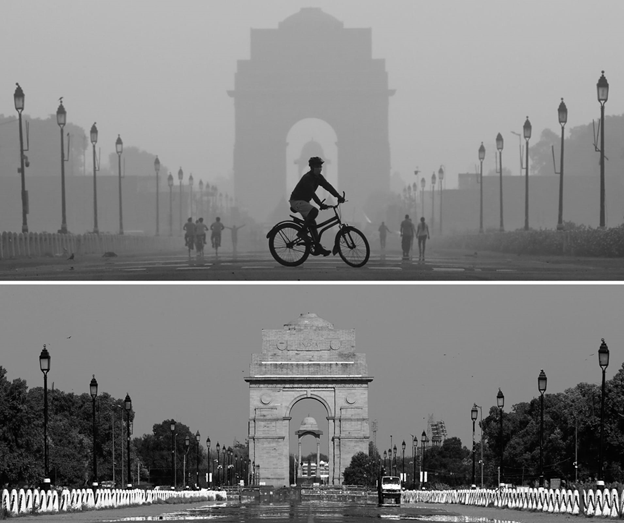
\includegraphics[width=0.6\linewidth]{images/air_pollution_greyscale} 

}

\caption{The India Gate in New Delhi, India.}\label{fig:covid}
\end{figure}

\vspace{.05in}

\begin{center}\includegraphics[width=0.6\linewidth]{10-paired_files/figure-latex/unnamed-chunk-2-1} \end{center}

\vspace{.2in}

\begin{longtable}[]{@{}ccll@{}}
\caption{Summary statistics for current AQI scores, median AQI scores from 2015--2019, and the differences in AQI scores.}\tabularnewline
\toprule
& Mean & Standard deviation & Sample size\tabularnewline
\midrule
\endfirsthead
\toprule
& Mean & Standard deviation & Sample size\tabularnewline
\midrule
\endhead
Current & \(\bar{x}_1\) = 47.394 & \(s_1\) = 14.107 & \(n_1\) = 33\tabularnewline
5 Year Median & \(\bar{x}_2\) = 51.545 & \(s_2\) = 17.447 & \(n_2\) = 33\tabularnewline
Differences & \(\bar{x}_d\) = -4.152 & \(s_d\) = 17.096 & \(n_d\) = 33\tabularnewline
\bottomrule
\end{longtable}

\newpage

\hypertarget{vocabulary-review.-complete-q1---5-before-class.}{%
\subsection*{Vocabulary review. Complete Q1 - 5 before class.}\label{vocabulary-review.-complete-q1---5-before-class.}}
\addcontentsline{toc}{subsection}{Vocabulary review. Complete Q1 - 5 before class.}

\begin{enumerate}
\def\labelenumi{\arabic{enumi}.}
\tightlist
\item
  What is the sample size?
\end{enumerate}

\vspace{0.5in}

\begin{enumerate}
\def\labelenumi{\arabic{enumi}.}
\setcounter{enumi}{1}
\tightlist
\item
  Identify the variables in this study. What role do each have?
\end{enumerate}

\vspace{.8in}

\begin{enumerate}
\def\labelenumi{\arabic{enumi}.}
\setcounter{enumi}{2}
\tightlist
\item
  Why is this treated as a paired study design and not two independent samples?
\end{enumerate}

\vspace{1in}

\begin{enumerate}
\def\labelenumi{\arabic{enumi}.}
\setcounter{enumi}{3}
\tightlist
\item
  Is this an experiment or observational study? Justify your answer.
\end{enumerate}

\vspace{0.3in}

\begin{enumerate}
\def\labelenumi{\arabic{enumi}.}
\setcounter{enumi}{4}
\tightlist
\item
  Are the differences in AQI scores independent for each case (US city)? Explain.
\end{enumerate}

\vspace{0.3in}

\hypertarget{ask-a-research-question}{%
\subsection*{Ask a research question}\label{ask-a-research-question}}
\addcontentsline{toc}{subsection}{Ask a research question}

\begin{enumerate}
\def\labelenumi{\arabic{enumi}.}
\setcounter{enumi}{5}
\tightlist
\item
  What are the two competing possibilities to run a hypothesis test for this study?
\end{enumerate}

\vspace{1in}

\begin{enumerate}
\def\labelenumi{\arabic{enumi}.}
\setcounter{enumi}{6}
\tightlist
\item
  Write the null hypothesis in words.
\end{enumerate}

\vspace{1in}

\begin{enumerate}
\def\labelenumi{\arabic{enumi}.}
\setcounter{enumi}{7}
\tightlist
\item
  What is the research question?
\end{enumerate}

\vspace{1in}

\begin{enumerate}
\def\labelenumi{\arabic{enumi}.}
\setcounter{enumi}{8}
\tightlist
\item
  Write the alternative hypothesis in notation.
\end{enumerate}

\vspace{1in}

\hypertarget{summarize-and-visualize-the-data}{%
\subsection*{Summarize and visualize the data}\label{summarize-and-visualize-the-data}}
\addcontentsline{toc}{subsection}{Summarize and visualize the data}

\begin{enumerate}
\def\labelenumi{\arabic{enumi}.}
\setcounter{enumi}{9}
\tightlist
\item
  Report the summary statistic for the data.
\end{enumerate}

\vspace{0.3in}

\begin{enumerate}
\def\labelenumi{\arabic{enumi}.}
\setcounter{enumi}{10}
\tightlist
\item
  What notation is used for the value in question 10?
\end{enumerate}

\vspace{0.3in}

\hypertarget{use-statistical-inferential-methods-to-draw-inferences-from-the-data}{%
\subsection*{Use statistical inferential methods to draw inferences from the data}\label{use-statistical-inferential-methods-to-draw-inferences-from-the-data}}
\addcontentsline{toc}{subsection}{Use statistical inferential methods to draw inferences from the data}

To simulate the null distribution we will use a bootstrapping method. Recall that the null distribution must be created under the assumption that the null hypothesis is true. Therefore, before bootstrapping we will need to shift each data point by the difference \(\mu_0 - \bar{x}\). This will ensure that the mean of the shifted data is \(\mu_0\) and that the simulated null distribution will be centered at the null value.

\begin{enumerate}
\def\labelenumi{\arabic{enumi}.}
\setcounter{enumi}{11}
\tightlist
\item
  Calculate the difference \(\mu_0 - \bar{x}\). Will we need to shift the data up or down?
\end{enumerate}

\vspace{.7in}

\begin{enumerate}
\def\labelenumi{\arabic{enumi}.}
\setcounter{enumi}{12}
\tightlist
\item
  Use the provided \texttt{RScript} file and enter the calculated value from question 12 for xx to simulate the null distribution and enter the summary statistic from question 10 for yy to find the p-value. Highlight and run lines 1 - 21.
\end{enumerate}

\begin{Shaded}
\begin{Highlighting}[]
    \KeywordTok{paired\_test}\NormalTok{(}\DataTypeTok{data =}\NormalTok{ Air}\OperatorTok{$}\NormalTok{Difference,   }\CommentTok{\#Vector of differences or data set with column for each group}
            \DataTypeTok{shift =}\NormalTok{ xx,   }\CommentTok{\#Shift needed for bootstrap hypothesis test}
            \DataTypeTok{as\_extreme\_as =}\NormalTok{ yy,  }\CommentTok{\#Observed statistic}
            \DataTypeTok{direction =} \StringTok{"less"}\NormalTok{,  }\CommentTok{\#Direction of alternative}
            \DataTypeTok{number\_repetitions =} \DecValTok{1000}\NormalTok{,  }\CommentTok{\#Number of simulated samples for null distribution}
            \DataTypeTok{which\_first =} \DecValTok{1}\NormalTok{)  }\CommentTok{\#Not needed when using calculated differences}
\end{Highlighting}
\end{Shaded}

\begin{enumerate}
\def\labelenumi{\arabic{enumi}.}
\setcounter{enumi}{13}
\tightlist
\item
  Sketch the null distribution created in question 13 here.
\end{enumerate}

\vspace{2in}

\begin{enumerate}
\def\labelenumi{\arabic{enumi}.}
\setcounter{enumi}{14}
\tightlist
\item
  Explain why the null distribution is centered at zero.
\end{enumerate}

\vspace{.5in}

\begin{enumerate}
\def\labelenumi{\arabic{enumi}.}
\setcounter{enumi}{15}
\tightlist
\item
  What proportion of samples are at or less than the sample mean difference in AQI scores for current scores minus 5 year median scores?
\end{enumerate}

\vspace{.3in}

\begin{enumerate}
\def\labelenumi{\arabic{enumi}.}
\setcounter{enumi}{16}
\tightlist
\item
  Interpret the p-value in the context of the problem.
\end{enumerate}

\vspace{.8in}

\begin{enumerate}
\def\labelenumi{\arabic{enumi}.}
\setcounter{enumi}{17}
\tightlist
\item
  How much evidence does this provide for improved air quality in U.S. cities?
\end{enumerate}

\vspace{.3in}

\begin{enumerate}
\def\labelenumi{\arabic{enumi}.}
\setcounter{enumi}{18}
\tightlist
\item
  Write out the parameter of interest in context of the study.
\end{enumerate}

\vspace{.6in}

\begin{enumerate}
\def\labelenumi{\arabic{enumi}.}
\setcounter{enumi}{19}
\tightlist
\item
  Using the provided \texttt{RScript} file fill in the missing value at xx in the paired bootstrap CI to find a 99\% confidence interval, highlight and run lines 24 - 27. Report the confidence interval in interval notation.
\end{enumerate}

\begin{Shaded}
\begin{Highlighting}[]
\KeywordTok{paired\_bootstrap\_CI}\NormalTok{(}\DataTypeTok{data =}\NormalTok{ Air}\OperatorTok{$}\NormalTok{Difference, }\CommentTok{\#Enter vector of differences}
                    \DataTypeTok{number\_repetitions =} \DecValTok{1000}\NormalTok{, }\CommentTok{\#Number of bootstrap samples for CI}
                    \DataTypeTok{confidence\_level =}\NormalTok{ xx,  }\CommentTok{\#Confidence level in decimal form}
                    \DataTypeTok{which\_first =} \DecValTok{1}\NormalTok{)  }\CommentTok{\#Not needed when entering vector of differences}
\end{Highlighting}
\end{Shaded}

\vspace{.3in}

\hypertarget{communicate-the-results-and-answer-the-research-question.}{%
\subsection*{Communicate the results and answer the research question.}\label{communicate-the-results-and-answer-the-research-question.}}
\addcontentsline{toc}{subsection}{Communicate the results and answer the research question.}

\begin{enumerate}
\def\labelenumi{\arabic{enumi}.}
\setcounter{enumi}{20}
\tightlist
\item
  Interpret the 99\% confidence interval in the context of the problem.
\end{enumerate}

\vspace{.8in}

\begin{enumerate}
\def\labelenumi{\arabic{enumi}.}
\setcounter{enumi}{21}
\tightlist
\item
  Do the results of your confidence interval and hypothesis test agree? What does each tell you about the null hypothesis?
\end{enumerate}

\vspace{.7in}

\begin{enumerate}
\def\labelenumi{\arabic{enumi}.}
\setcounter{enumi}{22}
\tightlist
\item
  Write a paragraph summarizes the results of this study. Be sure to describe:
\end{enumerate}

\begin{itemize}
\item
  Summary statistic
\item
  P-value and interpretation
\item
  Conclusion (written to answer the research question)
\item
  Confidence interval and interpretation
\item
  Scope of inference
\end{itemize}

\vspace{3in}

\hypertarget{revisit-and-look-forward}{%
\subsection*{Revisit and look forward}\label{revisit-and-look-forward}}
\addcontentsline{toc}{subsection}{Revisit and look forward}

\begin{enumerate}
\def\labelenumi{\arabic{enumi}.}
\setcounter{enumi}{23}
\tightlist
\item
  Would it be possible to design an experiment to determine if the changed human behavior due to the COVID-19 pandemic causes a decrease in air pollution? Explain.
  \vspace{0.6in}
\end{enumerate}

\newpage

\hypertarget{out-of-class-activity}{%
\section{Out of Class Activity}\label{out-of-class-activity}}

The remaining questions cover theory-based methods for testing paired quantitative data. Use section 6.2.3 in the textbook and the OneMeanTheory video to complete the following questions.

The sampling distribution for \(\bar{x}\) based on a sample of size \(n\) from a population with a true mean \(\mu\) and true standard deviation \(\sigma\) can be modeled using a normal distribution when certain conditions are met.

Conditions for the sample distribution of \(\bar{x}\).

\begin{itemize}
\item
  Independence: The sample's observations are independent
\item
  Normality: data should be approximately normal

  \begin{itemize}
  \item
    n \textless{} 30: If the sample size n is less than 30 and there are no clear outliers in the data, then we typically assume the data come from a nearly normal distribution to satisfy the condition.
  \item
    n ≥ 30: If the sample size n is at least 30 and there are no particularly extreme outliers, then we typically assume the sampling distribution of \(\bar{x}\) is nearly normal, even if the underlying distribution of individual observations is not.
  \end{itemize}
\end{itemize}

\begin{enumerate}
\def\labelenumi{\arabic{enumi}.}
\tightlist
\item
  In the in-class activity we verified that the independence condition was satisfied. Is the normality condition met to use the theory-based methods for analysis? Explain your answer.
\end{enumerate}

\vspace{1in}

To find the standardized statistic for the paired differences we will use the following formula:

\[T = \frac{\bar{x}_d}{SE(\bar{x}_d)}\]

where the standard error of the mean difference is:

\[SE(\bar{x}_d)=\frac{s_d}{\sqrt{n}}\]

\begin{enumerate}
\def\labelenumi{\arabic{enumi}.}
\setcounter{enumi}{1}
\tightlist
\item
  Calculate the standard error of the mean difference.
\end{enumerate}

\vspace{0.5in}

\begin{enumerate}
\def\labelenumi{\arabic{enumi}.}
\setcounter{enumi}{2}
\tightlist
\item
  Calculate the standardized statistic.
\end{enumerate}

\vspace{0.5in}

Using the provided \texttt{RScript} file, enter the T score (for xx) into the pt function using a df = minimum(n - 1) = 33 - 1 = 32, and lower.tail = TRUE to find the p-value. Highlight and run line 31.

\begin{Shaded}
\begin{Highlighting}[]
\KeywordTok{pt}\NormalTok{(xx, }\DataTypeTok{df=}\DecValTok{32}\NormalTok{, }\DataTypeTok{lower.tail=}\OtherTok{TRUE}\NormalTok{)}
\end{Highlighting}
\end{Shaded}

\begin{enumerate}
\def\labelenumi{\arabic{enumi}.}
\setcounter{enumi}{3}
\tightlist
\item
  Is the p-value found using theory-based methods similar to the simulation p-value found in the in-class activity?
\end{enumerate}

\vspace{0.5in}

To calculate the 99\% confidence interval use the following formula:

\[\bar{x}_d\pm t^* SE(\bar{x}_d)\]

We will need to find the \(t^*\) multiplier using the function qt. For a 99\% confidence interval we are finding the \(t^*\) value at the 99.5th percentile with df = n - 1 = 33 - 1 = 32.

\begin{Shaded}
\begin{Highlighting}[]
\KeywordTok{qt}\NormalTok{(}\FloatTok{0.995}\NormalTok{, }\DataTypeTok{df =} \DecValTok{32}\NormalTok{, }\DataTypeTok{lower.tail=}\OtherTok{TRUE}\NormalTok{)}
\CommentTok{\#\textgreater{} [1] 2.738481}
\end{Highlighting}
\end{Shaded}

\begin{enumerate}
\def\labelenumi{\arabic{enumi}.}
\setcounter{enumi}{4}
\tightlist
\item
  Calculate the 99\% confidence interval using theory-based methods.
\end{enumerate}

\vspace{1in}

\begin{enumerate}
\def\labelenumi{\arabic{enumi}.}
\setcounter{enumi}{5}
\tightlist
\item
  Explain why the theory-based and simulation confidence intervals are not quite the same.
\end{enumerate}

\vspace{1in}

\hypertarget{additional-notes}{%
\section{Additional notes}\label{additional-notes}}

Use this space to summarize your thoughts and take additional notes on today's activity.

\hypertarget{activity-11-weather-patterns-and-record-snowfall}{%
\chapter{Activity 11: Weather Patterns and Record Snowfall}\label{activity-11-weather-patterns-and-record-snowfall}}

\newcommand\latexcode[1]{#1}

\hypertarget{learning-objectives}{%
\section{Learning objectives}\label{learning-objectives}}

\begin{itemize}
\item
  Write out the null and alternative hypothesis for one categorical and one quantitative variable
\item
  Calculate and carry-out simulation based hypothesis test for a difference in means
\item
  Interpret and evaluate a p-value
\item
  Find a bootstrap confidence interval for a difference in means
\item
  Interpret a confidence interval
\item
  Use a confidence interval to determine the conclusion of a hypothesis test
\end{itemize}

\hypertarget{terminology-review}{%
\section{Terminology review}\label{terminology-review}}

In this week's in-class activity, we will use simulation-based methods to analyze one categorical and one quantitative variable, where the groups formed by the categorical variable are independent. Some terms covered in this activity are:

\begin{itemize}
\item
  Independent groups
\item
  Difference in means
\end{itemize}

To review these concepts, see Section 6.3 in the textbook.

\hypertarget{weather-patterns-and-record-snowfall}{%
\section{Weather patterns and record snowfall}\label{weather-patterns-and-record-snowfall}}

In the winter of 2018-2019, Bozeman had a record snowfall which resulted in the collapse of two flat-roofed buildings on the MSU campus. A writer for the Washington Post predicted the heavy snowfall for 2018-2019 due to the El Ni\~{n}o weather pattern that occurred in that season. A meteorologist in Montana wanted to see if the weather pattern really was associated with total snowfall. She obtained historical data from 44 years on the weather pattern (El Ni\~{n}o or La Ni\~{n}a) and snowfall (in inches) at the Billings Weather Station.

Notice from the \texttt{R} code that the name of the data set is \texttt{Snow}.

\begin{Shaded}
\begin{Highlighting}[]
\NormalTok{Snow \textless{}{-}}\StringTok{ }\KeywordTok{read.csv}\NormalTok{(}\StringTok{"data/SnowfallbyWeatherPattern.csv"}\NormalTok{) }\CommentTok{\# Read in data set}
\CommentTok{\# Code categorical variables as factors}
\NormalTok{Snow \textless{}{-}}\StringTok{ }\CommentTok{\# Write over original data with the following}
\StringTok{  }\NormalTok{Snow }\OperatorTok{\%\textgreater{}\%}\StringTok{ }\CommentTok{\# Pipe data set into}
\StringTok{  }\KeywordTok{mutate}\NormalTok{(}\DataTypeTok{WeatherPattern =} \KeywordTok{factor}\NormalTok{(WeatherPattern)) }\CommentTok{\# Convert to factor}
\end{Highlighting}
\end{Shaded}

\newpage

\begin{Shaded}
\begin{Highlighting}[]
\CommentTok{\# Side{-}by{-}side box plots}
\NormalTok{Snow }\OperatorTok{\%\textgreater{}\%}
\KeywordTok{ggplot}\NormalTok{(}\KeywordTok{aes}\NormalTok{(}\DataTypeTok{x =}\NormalTok{ WeatherPattern, }\DataTypeTok{y =}\NormalTok{ Snowfall)) }\OperatorTok{+}
\StringTok{    }\KeywordTok{geom\_boxplot}\NormalTok{() }\OperatorTok{+}\StringTok{ }
\StringTok{    }\KeywordTok{labs}\NormalTok{(}\DataTypeTok{title =} \StringTok{"Snowfall by weather pattern"}\NormalTok{,}
         \DataTypeTok{x =} \StringTok{"Weather pattern"}\NormalTok{) }\OperatorTok{+}
\StringTok{    }\KeywordTok{coord\_flip}\NormalTok{()}
\end{Highlighting}
\end{Shaded}

\begin{center}\includegraphics[width=0.6\linewidth]{11-inference-1ofeach_files/figure-latex/unnamed-chunk-2-1} \end{center}

\begin{Shaded}
\begin{Highlighting}[]
\CommentTok{\# Summary statistics}
\NormalTok{Snow }\OperatorTok{\%\textgreater{}\%}\StringTok{ }
\StringTok{     }\KeywordTok{summarize}\NormalTok{(}\KeywordTok{favstats}\NormalTok{(Snowfall}\OperatorTok{\textasciitilde{}}\NormalTok{WeatherPattern))}
\end{Highlighting}
\end{Shaded}

\begin{verbatim}
#>   WeatherPattern  min   Q1 median   Q3   max     mean       sd  n missing
#> 1        El_Nino 31.9 46.4   57.7 64.3  87.9 56.23043 13.00823 23       0
#> 2        La_Nina 44.5 51.4   60.9 70.3 107.2 63.13333 15.48626 21       0
\end{verbatim}

\hypertarget{quantitative-variables-review.-complete-q1---5-before-class.}{%
\subsection*{Quantitative variables review. Complete Q1 - 5 before class.}\label{quantitative-variables-review.-complete-q1---5-before-class.}}
\addcontentsline{toc}{subsection}{Quantitative variables review. Complete Q1 - 5 before class.}

\begin{enumerate}
\def\labelenumi{\arabic{enumi}.}
\tightlist
\item
  The two variables assessed in this study are the type of weather pattern and snowfall. Identify the role for each variable (explanatory, response).
\end{enumerate}

\vspace{.6in}

\begin{enumerate}
\def\labelenumi{\arabic{enumi}.}
\setcounter{enumi}{1}
\tightlist
\item
  Which group (El Ni\~{n}o or La Ni\~{n}a) has the highest center? Explain which measure of center you are using.
\end{enumerate}

\vspace{.6in}

\begin{enumerate}
\def\labelenumi{\arabic{enumi}.}
\setcounter{enumi}{2}
\tightlist
\item
  Using the side-by-side boxplots, which group has the largest spread? How did you make that choice?
\end{enumerate}

\vspace{.6in}

\newpage

\begin{enumerate}
\def\labelenumi{\arabic{enumi}.}
\setcounter{enumi}{3}
\tightlist
\item
  Is this an experiment or an observational study? Justify your answer.
\end{enumerate}

\vspace{1in}

\begin{enumerate}
\def\labelenumi{\arabic{enumi}.}
\setcounter{enumi}{4}
\tightlist
\item
  Is this a paired data set or two independent groups? Explain your reasoning.
\end{enumerate}

\vspace{1in}

\hypertarget{ask-a-research-question}{%
\subsection*{Ask a research question}\label{ask-a-research-question}}
\addcontentsline{toc}{subsection}{Ask a research question}

\begin{enumerate}
\def\labelenumi{\arabic{enumi}.}
\setcounter{enumi}{5}
\tightlist
\item
  Write out the parameter of interest in context of the study. Use proper notation and be sure to define your subscripts. Use El Ni\~{n}o minus La Ni\~{n}a as the order of subtraction.
\end{enumerate}

\vspace{1in}

\begin{enumerate}
\def\labelenumi{\arabic{enumi}.}
\setcounter{enumi}{6}
\tightlist
\item
  What are the two competing possibilities we will evaluate in this study?
\end{enumerate}

\vspace{1in}

\begin{enumerate}
\def\labelenumi{\arabic{enumi}.}
\setcounter{enumi}{7}
\tightlist
\item
  Identify which of your answers in question 7 is the null hypothesis and which is the alternative hypothesis.
\end{enumerate}

\vspace{1in}

\hypertarget{summarize-and-visualize-the-data}{%
\subsection*{Summarize and visualize the data}\label{summarize-and-visualize-the-data}}
\addcontentsline{toc}{subsection}{Summarize and visualize the data}

\begin{enumerate}
\def\labelenumi{\arabic{enumi}.}
\setcounter{enumi}{8}
\tightlist
\item
  Calculate the summary statistic. Use El Ni\~{n}o minus La Ni\~{n}a as the order of subtraction. What is the appropriate notation for the statistic?
\end{enumerate}

\vspace{0.5in}

\newpage

\hypertarget{use-statistical-inferential-methods-to-draw-inferences-from-the-data}{%
\subsection*{Use statistical inferential methods to draw inferences from the data}\label{use-statistical-inferential-methods-to-draw-inferences-from-the-data}}
\addcontentsline{toc}{subsection}{Use statistical inferential methods to draw inferences from the data}

Remember that the null distribution is created based on the assumption the null hypothesis is true. In this study, we assume there is no association between variables. This means that a snowfall value could be in either an El Ni\~{n}o year or a La Ni\~{n}a year.

To demonstrate this your instructor will use cards to represent the sample.

\begin{enumerate}
\def\labelenumi{\arabic{enumi}.}
\setcounter{enumi}{9}
\tightlist
\item
  How many cards will we start with?
\end{enumerate}

\vspace{0.5in}

\begin{enumerate}
\def\labelenumi{\arabic{enumi}.}
\setcounter{enumi}{10}
\tightlist
\item
  What will we write on each card?
\end{enumerate}

\vspace{0.5in}

\begin{enumerate}
\def\labelenumi{\arabic{enumi}.}
\setcounter{enumi}{11}
\tightlist
\item
  Next we will mix the cards together and shuffle into two piles. How many cards will go into each pile? What should we label the piles?
\end{enumerate}

\vspace{1in}

\begin{enumerate}
\def\labelenumi{\arabic{enumi}.}
\setcounter{enumi}{12}
\tightlist
\item
  What value is calculated from the cards and plotted on the null distribution? \emph{Hint}: What statistic are we calculating from the data?
\end{enumerate}

\vspace{0.3in}

\begin{enumerate}
\def\labelenumi{\arabic{enumi}.}
\setcounter{enumi}{13}
\tightlist
\item
  Once we create a null distribution of 1000 simulations, at what value do you expect the distribution to be centered? Explain your reasoning.
\end{enumerate}

\vspace{.8in}

\textbf{Simulation method}

\begin{enumerate}
\def\labelenumi{\arabic{enumi}.}
\setcounter{enumi}{14}
\tightlist
\item
  When using the two mean test we need to enter the name of the response variable, \texttt{Snowfall} and the name of the explanatory variable, \texttt{WeatherPattern} for the formula. The name of the data set as shown above is \texttt{Snow}. What values should be entered for each of the following into the two mean test to create 1000 simulations?
\end{enumerate}

\vspace{.2in}

\begin{itemize}
\tightlist
\item
  First in Subtraction (What is the outcome for the explanatory variable that is used as first in the order of subtraction? \texttt{"El\_Nino"} or \texttt{"La\_Nina"}:
\end{itemize}

\vspace{.2in}

\begin{itemize}
\tightlist
\item
  Number of repetitions:
\end{itemize}

\vspace{.2in}

\begin{itemize}
\tightlist
\item
  As extreme as:
\end{itemize}

\vspace{.2in}

\begin{itemize}
\tightlist
\item
  Direction (\texttt{"greater"}, \texttt{"less"}, or \texttt{"two-sided"}):
\end{itemize}

\vspace{.2in}

\begin{enumerate}
\def\labelenumi{\arabic{enumi}.}
\setcounter{enumi}{15}
\tightlist
\item
  Using the \texttt{RScript} file for this activity, enter your answers for question 15 in place of the xx's to produce the null distribution with 1000 simulations. Highlight and run lines 1 - 29.
\end{enumerate}

\begin{Shaded}
\begin{Highlighting}[]
\KeywordTok{two\_mean\_test}\NormalTok{(Snowfall}\OperatorTok{\textasciitilde{}}\NormalTok{WeatherPattern, }\DataTypeTok{data =}\NormalTok{ Snow,  }\CommentTok{\#Variables and data}
                    \DataTypeTok{first\_in\_subtraction =} \StringTok{"xx"}\NormalTok{, }\CommentTok{\#First outcome in order of subtraction}
                    \DataTypeTok{number\_repetitions =} \DecValTok{1000}\NormalTok{,  }\CommentTok{\#Number of simulations}
                    \DataTypeTok{as\_extreme\_as =}\NormalTok{ xx,  }\CommentTok{\#Observed statistic}
                    \DataTypeTok{direction =} \StringTok{"xx"}\NormalTok{)  }\CommentTok{\#Direction of alternative: "greater", "less", or "two{-}sided"}
\end{Highlighting}
\end{Shaded}

Sketch the null distribution created using the code above.
\vspace{1.5in}

\begin{enumerate}
\def\labelenumi{\arabic{enumi}.}
\setcounter{enumi}{16}
\tightlist
\item
  Report the p-value. How much evidence does the p-value provide against the null hypothesis?
\end{enumerate}

\vspace{0.5in}

\begin{enumerate}
\def\labelenumi{\arabic{enumi}.}
\setcounter{enumi}{17}
\tightlist
\item
  Using bootstrapping find a 95\% confidence interval. Use the provided \texttt{RScript} file for the two mean bootstrap CI function. Enter the variable names and data set name as in the two mean test, outcome name for the first in subtraction, number of repetitions, and the confidence level as a decimal. Highlight and run lines 32 - 35. Report the 95\% confidence interval in interval notation.
\end{enumerate}

\begin{Shaded}
\begin{Highlighting}[]
\KeywordTok{two\_mean\_bootstrap\_CI}\NormalTok{(RESPONSE}\OperatorTok{\textasciitilde{}}\NormalTok{EXPLANATORY, }\DataTypeTok{data =}\NormalTok{ DATASET,  }\CommentTok{\#Variables and data}
                      \DataTypeTok{first\_in\_subtraction =} \StringTok{"xx"}\NormalTok{, }\CommentTok{\#First value in order of subtraction}
                      \DataTypeTok{number\_repetitions =} \DecValTok{1000}\NormalTok{,  }\CommentTok{\#Number of simulations}
                      \DataTypeTok{confidence\_level =}\NormalTok{ xx)}
\end{Highlighting}
\end{Shaded}

\vspace{0.3in}

\begin{enumerate}
\def\labelenumi{\arabic{enumi}.}
\setcounter{enumi}{18}
\tightlist
\item
  Interpret the interval you calculated in question 18.
\end{enumerate}

\vspace{1in}

\hypertarget{communicate-the-results-and-answer-the-research-question}{%
\subsection*{Communicate the results and answer the research question}\label{communicate-the-results-and-answer-the-research-question}}
\addcontentsline{toc}{subsection}{Communicate the results and answer the research question}

\begin{enumerate}
\def\labelenumi{\arabic{enumi}.}
\setcounter{enumi}{19}
\tightlist
\item
  Write a paragraph summarizing the results of the study. Be sure to describe:
\end{enumerate}

\begin{itemize}
\item
  Summary statistic
\item
  P-value and interpretation
\item
  Conclusion (written to answer the research question)
\item
  Confidence interval and interpretation
\item
  Scope of inference
\end{itemize}

\vspace{3in}

\hypertarget{revisit-and-look-forward}{%
\subsection*{Revisit and look forward}\label{revisit-and-look-forward}}
\addcontentsline{toc}{subsection}{Revisit and look forward}

\begin{enumerate}
\def\labelenumi{\arabic{enumi}.}
\setcounter{enumi}{20}
\tightlist
\item
  Would the results from the theory-based test match the results we saw with the simulation? Explain why or why not.
\end{enumerate}

\vspace{1in}

\begin{enumerate}
\def\labelenumi{\arabic{enumi}.}
\setcounter{enumi}{21}
\tightlist
\item
  If we had data on 45 La Ni\~{n}a years and 47 El Ni\~{n}o years and found a similar summary statistic, what would happen to the p-value? The width of the confidence interval? The power of the test?
\end{enumerate}

\vspace{1in}

\hypertarget{out-of-class-activity}{%
\section{Out of Class Activity}\label{out-of-class-activity}}

The remaining questions cover inference for a difference in means using theory based methods. Use section 6.3.3 in the textbook and the TwoMeanTheory video to complete the following questions.

The sampling distribution for \(\bar{x}_1-\bar{x}_2\) can be modeled using a normal distribution when certain conditions are met.

Conditions for the sample distribution of \(\bar{x}_1-\bar{x}_2\).

\begin{itemize}
\item
  Independence: The sample's observations are independent
\item
  Normality: each sample should be approximately normal

  \begin{itemize}
  \item
    For each sample:

    \begin{itemize}
    \item
      \(n < 30\): If the sample size n is less than 30 and there are no clear outliers in the data, then we typically assume the data come from a nearly normal distribution to satisfy the condition.
    \item
      \(n \le 30\): If the sample size n is at least 30 and there are no particularly extreme outliers, then we typically assume the sampling distribution of \(\bar{x}\) is nearly normal, even if the underlying distribution of individual observations is not.
    \end{itemize}
  \end{itemize}
\end{itemize}

\begin{enumerate}
\def\labelenumi{\arabic{enumi}.}
\tightlist
\item
  In question 21 in the in-class activity we noted that there were issues with the normality condition. Explain how that will affect the p-value and confidence interval found with theory-based methods.
\end{enumerate}

\vspace{1in}

To find the Standardized Statistic for the difference in means we will calculate:

\[T = \frac{\bar{x}_1-\bar{x}_2}{SE(\bar{x}_1-\bar{x}_2)}\]

where the standard error of the difference in means is calculated using:

\[SE(\bar{x}_1 -\bar{x}_2)=\sqrt{\frac{s_1^2}{n_1}+\frac{s_2^2}{n_2}}\]
\newpage

\begin{enumerate}
\def\labelenumi{\arabic{enumi}.}
\setcounter{enumi}{1}
\tightlist
\item
  Calculate the standard error of the difference in means.
\end{enumerate}

\vspace{0.5in}

\begin{enumerate}
\def\labelenumi{\arabic{enumi}.}
\setcounter{enumi}{2}
\tightlist
\item
  Calculate the standardized statistic for the difference in means.
\end{enumerate}

\vspace{0.5in}

Using the provided \texttt{RScript} file, enter the T score (for xx) into the pt function using a df = minimum(n - 1) = 21 - 1 = 20, and lower.tail = TRUE to find the p-value. Highlight and run line 39.

\begin{Shaded}
\begin{Highlighting}[]
\DecValTok{2}\OperatorTok{*}\KeywordTok{pt}\NormalTok{(xx, }\DataTypeTok{df=}\DecValTok{20}\NormalTok{, }\DataTypeTok{lower.tail=}\OtherTok{TRUE}\NormalTok{)}
\end{Highlighting}
\end{Shaded}

\begin{enumerate}
\def\labelenumi{\arabic{enumi}.}
\setcounter{enumi}{3}
\tightlist
\item
  Explain why we multiplied by 2 in the code above.
\end{enumerate}

\vspace{0.3in}

\begin{enumerate}
\def\labelenumi{\arabic{enumi}.}
\setcounter{enumi}{4}
\tightlist
\item
  Report the p-value from the \texttt{R} output.
\end{enumerate}

\vspace{0.3in}

\begin{enumerate}
\def\labelenumi{\arabic{enumi}.}
\setcounter{enumi}{5}
\tightlist
\item
  Explain why the p-value found using theory-based methods from the p-value found using simulation methods in the in-class activity.
\end{enumerate}

\vspace{0.5in}

To calculate the 95\% confidence interval use the formula:

\[\bar{x}_1- \bar{x}_2\pm t^* SE(\bar{x}_1- \bar{x}_2)\]

We will need to find the \(t^*\) multiplier using the function qt. For a 95\% confidence interval we are finding the \(t^*\) value at the 97.5th percentile with df = minimum(n - 1) = 21 - 1 = 20.

\begin{Shaded}
\begin{Highlighting}[]
\KeywordTok{qt}\NormalTok{(}\FloatTok{0.975}\NormalTok{, }\DataTypeTok{df =} \DecValTok{20}\NormalTok{, }\DataTypeTok{lower.tail=}\OtherTok{TRUE}\NormalTok{)}
\CommentTok{\#\textgreater{} [1] 2.085963}
\end{Highlighting}
\end{Shaded}

\begin{enumerate}
\def\labelenumi{\arabic{enumi}.}
\setcounter{enumi}{6}
\tightlist
\item
  Calculate the 95\% confidence interval using theory-based methods.
\end{enumerate}

\vspace{1in}

\newpage

\hypertarget{additional-notes}{%
\section{Additional notes}\label{additional-notes}}

Use this space to summarize your thoughts and take additional notes on today's activity.

\hypertarget{activity-12-moneyball}{%
\chapter{Activity 12: Moneyball}\label{activity-12-moneyball}}

\hypertarget{learning-outcomes}{%
\section{Learning outcomes}\label{learning-outcomes}}

\begin{itemize}
\item
  Given a research question, construct the null and alternative hypotheses
  in words and using appropriate statistical symbols
\item
  Describe and perform theory-based hypothesis tests for the slope
\item
  Interpret and evaluate a p-value
\item
  Construct and interpret a theory-based confidence interval for slope
\item
  Use a confidence interval to determine the conclusion of a hypothesis test
\end{itemize}

\hypertarget{terminology-review}{%
\section{Terminology review}\label{terminology-review}}

In this week's in-class activity, we will use theory-based methods for hypothesis tests and confidence intervals for linear regression slope. Some terms covered in this activity are:

\begin{itemize}
\item
  Correlation
\item
  Slope
\item
  Regression line
\end{itemize}

To review these concepts, see Chapters 3 and 7 in the textbook.

\newpage

\hypertarget{moneyball}{%
\section{Moneyball}\label{moneyball}}

The goal of a Major League baseball team is to make the playoffs. In 2002, the manager of the Oakland A's, Billy Beane with the help of Paul DePodesta began to use statistics to determine which players to choose for their season. Based on past data, Paul determined that to make it to the playoffs, the A's would need to win at least 95 games in the regular season. In order to win more games they would need to score more runs than they allowed. In this study, we will see if there is evidence of a positive linear relationship between the difference in the number of runs scored minus the number of runs allowed and the number of wins for teams in the years before 2002.

The Oakland A's won 20 consecutive games and a total of 103 games for the season. The success of this use of sports analytics was portrayed by the 2011 movie, \emph{Moneyball}.

Some of the variables collected in this data set consist of the following:

\begin{longtable}[]{@{}ll@{}}
\toprule
\textbf{Variable} & \textbf{Description}\tabularnewline
\midrule
\endhead
\texttt{RA} & Runs allowed\tabularnewline
\texttt{RS} & Runs scored\tabularnewline
\texttt{OBP} & On Base Percentage\tabularnewline
\texttt{SLG} & Slugging Percentage\tabularnewline
\texttt{BA} & Batting Average\tabularnewline
\texttt{OOBP} & Opponent's On Base Percentage\tabularnewline
\texttt{OSLG} & Opponent's Slugging Percentage\tabularnewline
\texttt{W} & Number of Wins in the season\tabularnewline
\texttt{RD} & Difference of runs scored minus runs allowed\tabularnewline
\bottomrule
\end{longtable}

\begin{Shaded}
\begin{Highlighting}[]
\CommentTok{\# Read in data set}
\NormalTok{baseball \textless{}{-}}\StringTok{ }\KeywordTok{read.csv}\NormalTok{(}\StringTok{"data/baseball.csv"}\NormalTok{)}

\NormalTok{baseball}\OperatorTok{$}\NormalTok{RD \textless{}{-}}\StringTok{ }\NormalTok{baseball}\OperatorTok{$}\NormalTok{RS }\OperatorTok{{-}}\StringTok{ }\NormalTok{baseball}\OperatorTok{$}\NormalTok{RA }\CommentTok{\#create variable run difference}

\CommentTok{\# Code categorical variables as factors}
\NormalTok{baseball \textless{}{-}}\StringTok{ }\CommentTok{\# Write over original data with the following}
\StringTok{  }\NormalTok{baseball }\OperatorTok{\%\textgreater{}\%}\StringTok{ }\CommentTok{\# Pipe data set into}
\StringTok{  }\KeywordTok{subset}\NormalTok{(Year }\OperatorTok{\textless{}}\StringTok{ }\DecValTok{2002}\NormalTok{) }\CommentTok{\# Select only years before 2002}
\end{Highlighting}
\end{Shaded}

\hypertarget{vocabulary-review.-complete-q1---4-before-class.}{%
\subsection*{Vocabulary review. Complete Q1 - 4 before class.}\label{vocabulary-review.-complete-q1---4-before-class.}}
\addcontentsline{toc}{subsection}{Vocabulary review. Complete Q1 - 4 before class.}

\begin{enumerate}
\def\labelenumi{\arabic{enumi}.}
\tightlist
\item
  Explain why regression methods are appropriate to use to address the researchers' question. Make sure you clearly define the variables of interest in your explanation and their roles.
\end{enumerate}

\newpage

\begin{enumerate}
\def\labelenumi{\arabic{enumi}.}
\setcounter{enumi}{1}
\item
  Use the provided \texttt{RScript} file to create a scatterplot to examine the relationship between the difference in number of runs scored minus number of runs allowed and the number of wins by filling in the variable names (\texttt{RD} and \texttt{W}) for xx and yy in line 17. Highlight and run lines 1 - 22.

\begin{Shaded}
\begin{Highlighting}[]
\NormalTok{baseball }\OperatorTok{\%\textgreater{}\%}\StringTok{ }\CommentTok{\# Pipe data set into...}
\KeywordTok{ggplot}\NormalTok{(}\KeywordTok{aes}\NormalTok{(}\DataTypeTok{x =}\NormalTok{ xx, }\DataTypeTok{y =}\NormalTok{ yy))}\OperatorTok{+}\StringTok{  }\CommentTok{\#Specify variables}
\StringTok{  }\KeywordTok{geom\_point}\NormalTok{() }\OperatorTok{+}\StringTok{  }\CommentTok{\#Add scatterplot of points}
\StringTok{  }\KeywordTok{labs}\NormalTok{(}\DataTypeTok{x =} \StringTok{"Difference in number of runs"}\NormalTok{,  }\CommentTok{\#Label x{-}axis}
       \DataTypeTok{y =} \StringTok{"Number of wins"}\NormalTok{,  }\CommentTok{\#Label y{-}axis}
       \DataTypeTok{title =} \StringTok{"Scatterplot of Run Difference vs. Number of Wins"}\NormalTok{) }\OperatorTok{+}\StringTok{ }\CommentTok{\#Be sure to tile your plots}
\StringTok{  }\KeywordTok{geom\_smooth}\NormalTok{(}\DataTypeTok{method =} \StringTok{"lm"}\NormalTok{, }\DataTypeTok{se =} \OtherTok{FALSE}\NormalTok{)  }\CommentTok{\#Add regression line}
\end{Highlighting}
\end{Shaded}
\item
  Sketch the plot created below. Based on your plot, does it appear that there is a relationship between \texttt{run\ difference} and \texttt{wins}? Note: \texttt{RD} should be on the x-axis.
\end{enumerate}

\vspace{2in}

\begin{enumerate}
\def\labelenumi{\arabic{enumi}.}
\setcounter{enumi}{3}
\tightlist
\item
  Describe the features of the plot above.
\end{enumerate}

\vspace{1in}

~~~~~~~If you indicated there are potential outliers, which points are they?

\vspace{0.5in}

\hypertarget{conditions-for-the-least-squares-line}{%
\subsection*{Conditions for the least squares line}\label{conditions-for-the-least-squares-line}}
\addcontentsline{toc}{subsection}{Conditions for the least squares line}

When performing inference on a least squares line, the follow conditions are generally required

\begin{itemize}
\item
  Linearity: the data should follow a linear trend
\item
  Nearly normal residuals: residuals must be nearly normal
\item
  Constant variability: the variability of points around the least squares line remains roughly constant
\item
  Independent observations: individual data points must be independent
\end{itemize}

The scatterplot and the residual plots will be used to assess the conditions for approximating the data with the \(t\)-distribution.

\begin{center}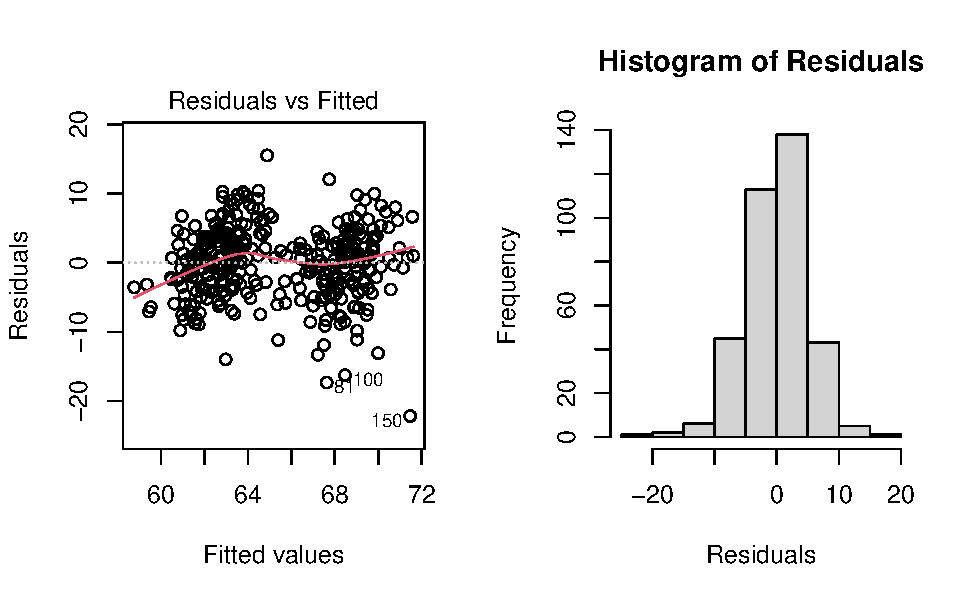
\includegraphics[width=0.7\linewidth]{12-regression_files/figure-latex/unnamed-chunk-3-1} \end{center}

\begin{enumerate}
\def\labelenumi{\arabic{enumi}.}
\setcounter{enumi}{4}
\tightlist
\item
  Are the conditions met to use the \(t\)-distribution to approximate the sampling distribution of the standardized statistic?
\end{enumerate}

\vspace{1.5in}

\hypertarget{ask-a-research-question}{%
\subsection*{Ask a research question}\label{ask-a-research-question}}
\addcontentsline{toc}{subsection}{Ask a research question}

\begin{enumerate}
\def\labelenumi{\arabic{enumi}.}
\setcounter{enumi}{5}
\tightlist
\item
  Write out the null hypothesis in words.
\end{enumerate}

\vspace{1in}

\begin{enumerate}
\def\labelenumi{\arabic{enumi}.}
\setcounter{enumi}{6}
\tightlist
\item
  Using the research question, write the alternative hypothesis in notation to test the slope.
\end{enumerate}

\vspace{0.5in}

\hypertarget{summarize-and-visualize-the-data}{%
\subsection*{Summarize and visualize the data}\label{summarize-and-visualize-the-data}}
\addcontentsline{toc}{subsection}{Summarize and visualize the data}

Using the provided \texttt{RScript} file, enter the response variable name, \texttt{W} into the linear model function for yy and the explanatory variable name, \texttt{RD} for xx in line 32 to get the linear model output. Highlight and run lines 32 - 33.

\begin{Shaded}
\begin{Highlighting}[]
\NormalTok{lm.baseball \textless{}{-}}\StringTok{ }\KeywordTok{lm}\NormalTok{(yy}\OperatorTok{\textasciitilde{}}\NormalTok{xx, }\DataTypeTok{data=}\NormalTok{baseball) }\CommentTok{\#lm(response\textasciitilde{}explanatory)}
\KeywordTok{round}\NormalTok{(}\KeywordTok{summary}\NormalTok{(lm.baseball)}\OperatorTok{$}\NormalTok{coefficients, }\DecValTok{5}\NormalTok{)}
\end{Highlighting}
\end{Shaded}

\begin{enumerate}
\def\labelenumi{\arabic{enumi}.}
\setcounter{enumi}{7}
\tightlist
\item
  Using the output from the evaluated \texttt{R} code above, write the equation of the regression line.
\end{enumerate}

\vspace{1in}

\begin{enumerate}
\def\labelenumi{\arabic{enumi}.}
\setcounter{enumi}{8}
\tightlist
\item
  Interpret the slope in context of the problem.
\end{enumerate}

\vspace{1in}

\begin{enumerate}
\def\labelenumi{\arabic{enumi}.}
\setcounter{enumi}{9}
\tightlist
\item
  Using your estimated line of best fit, predict the number of wins for a run difference of 147. Show all work.
\end{enumerate}

\vspace{1in}

\begin{enumerate}
\def\labelenumi{\arabic{enumi}.}
\setcounter{enumi}{10}
\tightlist
\item
  In 2002 the Oakland A's had a run difference of 147 and 103 wins. Calculate the residual associated with the observation (147, 103), using your estimated regression line from question 8.
\end{enumerate}

\vspace{1in}

\hypertarget{use-statistical-inferential-methods-to-draw-inferences-from-the-data}{%
\subsection*{Use statistical inferential methods to draw inferences from the data}\label{use-statistical-inferential-methods-to-draw-inferences-from-the-data}}
\addcontentsline{toc}{subsection}{Use statistical inferential methods to draw inferences from the data}

To find the value of the standardized statistic to test the slope we will use,

\[
T = \frac{\mbox{slope estimate}}{SE} = \frac{b_1}{SE(b_1)}
\]

We will use the linear model output above to get the estimate for slope and standard error of the slope.

\begin{enumerate}
\def\labelenumi{\arabic{enumi}.}
\setcounter{enumi}{11}
\tightlist
\item
  Calculate the standardized statistic for slope. Identify where this calculated value is in the linear model output.
\end{enumerate}

\vspace{1in}

\begin{enumerate}
\def\labelenumi{\arabic{enumi}.}
\setcounter{enumi}{12}
\tightlist
\item
  Interpret the standardized statistic in context of the problem.
\end{enumerate}

\vspace{0.8in}

\begin{enumerate}
\def\labelenumi{\arabic{enumi}.}
\setcounter{enumi}{13}
\tightlist
\item
  Using the linear model output, report the p-value for the test of significance.
\end{enumerate}

\vspace{0.5in}

\begin{enumerate}
\def\labelenumi{\arabic{enumi}.}
\setcounter{enumi}{14}
\tightlist
\item
  Based on the p-value, how much evidence is there against the null hypothesis?
\end{enumerate}

\vspace{0.5in}

Recall that a confidence interval is calculated by adding and subtracting the margin of error to the point estimate.\\
\[\mbox{point estimate}\pm t^*SE(estimate)\]
\[b_1 \pm t^* SE(b_1)\]

The \(t^*\) multiplier comes from the \(t\)-distribution with \(n-2\) df. Recall for a 95\% confidence interval, we use the 97.5\% percentile (95\% of the distribution is in the middle, leaving 2.5\% in each tail). The sample size for this study is 902 so we will use the degrees of freedom 900 (\(n-2\)).

\begin{Shaded}
\begin{Highlighting}[]
\KeywordTok{qt}\NormalTok{(}\FloatTok{0.95+0.025}\NormalTok{, }\DecValTok{900}\NormalTok{) }\CommentTok{\#95\% t* multiplier }
\end{Highlighting}
\end{Shaded}

\begin{verbatim}
#> [1] 1.962603
\end{verbatim}

\begin{enumerate}
\def\labelenumi{\arabic{enumi}.}
\setcounter{enumi}{15}
\item
  Calculate the 95\% confidence interval for the true slope.
  \vspace{0.8in}
\item
  Interpret the 95\% confidence interval in context of the problem.
\end{enumerate}

\vspace{1in}

\hypertarget{communicate-the-results-and-answer-the-research-question}{%
\subsection*{Communicate the results and answer the research question}\label{communicate-the-results-and-answer-the-research-question}}
\addcontentsline{toc}{subsection}{Communicate the results and answer the research question}

\begin{enumerate}
\def\labelenumi{\arabic{enumi}.}
\setcounter{enumi}{17}
\tightlist
\item
  Based on the p-value, write a conclusion in context of the problem.
\end{enumerate}

\vspace{1in}

\begin{enumerate}
\def\labelenumi{\arabic{enumi}.}
\setcounter{enumi}{18}
\tightlist
\item
  Does the p-value agree with the 95\% confidence interval? What does each tell you about the null hypothesis?
\end{enumerate}

\vspace{1in}

\begin{enumerate}
\def\labelenumi{\arabic{enumi}.}
\setcounter{enumi}{19}
\tightlist
\item
  Summarize the results of the study in a written paragraph. Be sure to describe:
\end{enumerate}

\begin{itemize}
\item
  Summary statistic
\item
  Test statistic and interpretation
\item
  P-value and interpretation
\item
  Confidence interval and interpretation
\item
  Conclusion (written to answer the research question)
\item
  Scope of inference
\end{itemize}

\vspace{3in}

\newpage

\hypertarget{revisit-and-look-forward}{%
\subsection*{Revisit and look forward}\label{revisit-and-look-forward}}
\addcontentsline{toc}{subsection}{Revisit and look forward}

In order to see what team attributes would have the most impact on the number of runs scored, Beane and DePodesta created several prediction models. Using 2001 statistics, they looked at a prediction model using both the team's on base percentage and slugging percentage to predict the number of runs scored. The following \texttt{R} code gives the estimates for the regression model with both of these variables included.

\begin{Shaded}
\begin{Highlighting}[]
\NormalTok{lm.score \textless{}{-}}\StringTok{ }\KeywordTok{lm}\NormalTok{(RS}\OperatorTok{\textasciitilde{}}\NormalTok{OBP}\OperatorTok{+}\NormalTok{SLG, }\DataTypeTok{data=}\NormalTok{baseball)}
\KeywordTok{round}\NormalTok{(}\KeywordTok{summary}\NormalTok{(lm.score)}\OperatorTok{$}\NormalTok{coefficients, }\DecValTok{5}\NormalTok{)}
\CommentTok{\#\textgreater{}              Estimate Std. Error   t value Pr(\textgreater{}|t|)}
\CommentTok{\#\textgreater{} (Intercept) {-}804.6271   18.92079 {-}42.52608        0}
\CommentTok{\#\textgreater{} OBP         2737.7680   90.68455  30.19001        0}
\CommentTok{\#\textgreater{} SLG         1584.9086   42.15559  37.59665        0}
\end{Highlighting}
\end{Shaded}

\begin{enumerate}
\def\labelenumi{\arabic{enumi}.}
\setcounter{enumi}{20}
\tightlist
\item
  Use the provided \texttt{R} output to write the linear regression model including all variables. \emph{Hint}: The estimated line of regression is:
\end{enumerate}

\[\widehat{\text{runs scored}} = b_0 + b_1*OBP + b_2*SLG\]

\vspace{1in}

\begin{enumerate}
\def\labelenumi{\arabic{enumi}.}
\setcounter{enumi}{21}
\tightlist
\item
  Using the line of regression above, predict the number of runs for the Oakland A's in 2002 if the team OBP is 0.339 and the team SLPG is 0.430.
\end{enumerate}

\vspace{1in}

\hypertarget{out-of-class-activity}{%
\section{Out of class activity}\label{out-of-class-activity}}

In the out of class activity we will focus on using simulation based methods for inference of regression. Use section 7.1 in the textbook and the TwoQuantSim video to complete the following questions.

First let's think about how one simulation would be created on the null distribution using cards. First we would write the values for the response variable, wins, on each card. Next, we would shuffle the y values to a new x value (explanatory variable). Then, find the line of regression for the shuffled cards.

\begin{enumerate}
\def\labelenumi{\arabic{enumi}.}
\tightlist
\item
  Once we have one simulated sample, what would we calculate and plot on the null distribution? \emph{Hint}: What statistic are we calculating from the data?
\end{enumerate}

\vspace{1in}

To create the null distribution, we will use the regression test from the catstats package. We will need to enter the response variable name and the explanatory variable name for the formula, the data set name identified above as \texttt{baseball}, the statistic for the test (either slope or correlation), number of repetitions, the sample statistic (value of slope or correlation), and the direction of the alternative hypothesis.

The response variable name is \texttt{W} (wins) and the explanatory variable name is \texttt{RD} (run difference).

\begin{enumerate}
\def\labelenumi{\arabic{enumi}.}
\setcounter{enumi}{1}
\tightlist
\item
  What inputs should be entered for each of the following to create the simulation?
\end{enumerate}

\vspace{.5 mm}

\begin{itemize}
\tightlist
\item
  Direction (\texttt{"greater"}, \texttt{"less"}, or \texttt{"two-sided"}):
\end{itemize}

\vspace{.2in}

\begin{itemize}
\tightlist
\item
  Statistic (choose \texttt{"slope"} or \texttt{"correlation"}):
\end{itemize}

\vspace{.2in}

\begin{itemize}
\tightlist
\item
  As extreme as (enter the value for the sample slope):
\end{itemize}

\vspace{0.2in}

\begin{itemize}
\tightlist
\item
  Number of repetitions:
\end{itemize}

\vspace{.2in}

Using the \texttt{RScript} file for this activity, enter your answers for question 2 in place of the xx's for the regression test to produce the null distribution with 1000 simulations. Highlight and run lines 1 - 13 and then lines 44-49.

\begin{Shaded}
\begin{Highlighting}[]
\KeywordTok{regression\_test}\NormalTok{(W}\OperatorTok{\textasciitilde{}}\NormalTok{RD, }\CommentTok{\# response \textasciitilde{} explanatory}
               \DataTypeTok{data =}\NormalTok{ baseball, }\CommentTok{\# name of data set}
               \DataTypeTok{direction =} \StringTok{"xx"}\NormalTok{, }\CommentTok{\# sign in alternative ("greater", "less", "two{-}sided")}
               \DataTypeTok{statistic =} \StringTok{"xx"}\NormalTok{, }
               \DataTypeTok{as\_extreme\_as =}\NormalTok{ x, }\CommentTok{\#observed slope}
               \DataTypeTok{number\_repetitions =} \DecValTok{1000}\NormalTok{) }\CommentTok{\#Number of simulated samples for null distribution}
       
\end{Highlighting}
\end{Shaded}

\begin{enumerate}
\def\labelenumi{\arabic{enumi}.}
\setcounter{enumi}{2}
\tightlist
\item
  Report the p-value from the \texttt{R} output. Is this value similar to what was seen with the theory-based methods?
\end{enumerate}

\vspace{0.5in}

Fill in the xx's in the regression bootstrap CI function in the provided \texttt{RScript} file to find a 95\% confidence interval. Highlight and run lines 52-56.

\begin{Shaded}
\begin{Highlighting}[]
\KeywordTok{regression\_bootstrap\_CI}\NormalTok{(W}\OperatorTok{\textasciitilde{}}\NormalTok{RD, }\CommentTok{\# response \textasciitilde{} explanatory}
                        \DataTypeTok{data =}\NormalTok{ baseball, }\CommentTok{\# name of data set}
                        \DataTypeTok{confidence\_level =}\NormalTok{ xx, }\CommentTok{\# confidence level as decimal}
                        \DataTypeTok{statistic =} \StringTok{"xx"}\NormalTok{, }\CommentTok{\# slope or correlation}
                        \DataTypeTok{number\_repetitions =} \DecValTok{1000}\NormalTok{) }\CommentTok{\#Number of simulated samples for bootstrap distribution}
\end{Highlighting}
\end{Shaded}

\begin{enumerate}
\def\labelenumi{\arabic{enumi}.}
\setcounter{enumi}{3}
\item
  Report the bootstrap 95\% confidence interval in interval notation.\\
  \vspace{0.5in}
\item
  Is the bootstrap 95\% confidence interval similar to what was found using theory-based methods? Why did you expect this to be true?
\end{enumerate}

\vspace{1in}

\hypertarget{additional-notes}{%
\section{Additional notes}\label{additional-notes}}

Use this space to summarize your thoughts and take additional notes on today's activity.

\end{document}
